% \documentclass[12pt]{diss_4}
\documentclass[a6paper, 11pt]{diss_4}
\usepackage{mathtext}
\usepackage{amssymb,amsmath}
\usepackage[active]{srcltx}
%*****************************%
\usepackage[utf8x]{inputenc}
\usepackage[english,russian]{babel}
%\usepackage{literat}
\usepackage{array}
\usepackage{booktabs}
%\usepackage{floatfig}
\usepackage{wrapfig}

\usepackage{graphicx}
%  \usepackage{geometry}
%  \geometry{left=1.5cm}
 % \geometry{right=1.5cm}
 % \geometry{top=2cm}
 % \geometry{bottom=2cm}
%*****************************%
% \setlength{\topmargin}{-37mm}
% \setlength{\oddsidemargin}{-24,5mm}
%\pagestyle{empty}
%\mathsurround=1mm
\tolerance=1000
\emergencystretch=5pt
%*****************************%
 % \textheight=17cm
 % \textwidth=10,9cm
% \textheight=24cm.
% \textwidth=18cm
% \hoffset=2cm
% \voffset=2cm
\setlength{\parskip}{6pt}
%*****************************%
\newcommand{\kmh}{$\frac{км}{ч}$\ }
\newcommand{\ms}{$\frac{м}{с}$\ }
\newcommand{\lh}{$\frac{л}{ч}$\ }
\newcommand{\ls}{$\frac{л}{с}$\ }
\newcommand{\mks}{$\frac{м^3}{с}$\ }
\newcommand{\mkm}{$\frac{м^3}{мин}$\ }
\newcommand{\mkh}{$\frac{м^3}{ч}$\ }
\newcommand{\smm}{$\frac{см}{мин}$\ }
\newcommand{\smkvm}{$\frac{см^2}{мин}$\ }
\newcommand{\mkvs}{$\frac{см^2}{с}$\ }
\newcommand{\TNF}{$\vec{F}=m\vec{a}$}
\newcommand{\TNFN}{\vec{F}=m\vec{a}}
\renewcommand{\'}{\,'}
\newcommand{\UDV}{\vec{S}=\vec{v}_0t+\frac{\vec{a}t^2}{2}}
%*****************************%

\begin{document}
\begin{titlepage}
\vspace*{1cm}
\begin{center}

 БИБИКОВ\ Дмитрий Николаевич
\vspace{1mm}

 Компьютерная верстка: \\
\vspace{2mm}
 САРАФАНОВ Федор Георгиевич
\vspace{3mm}

\end{center}

\vspace{2cm}

\begin{center}
 \bf
\Huge{  ФИЗИКА  }   \\
\large{ 9 класс, учебное пособие}
\end{center}

\vfill

\begin{center}
Нижний Новгород

2013
\end{center}
\end{titlepage}
\addtocounter{page}{1}
\tableofcontents
%\large
\chapter{Законы взаимодействия и движения тел}
\section{Понятие о материи}

 Физика - одна из ведущих естественных наук. <<Фюзис>> с греческого - природа.
Всё, что окружает нас, мы называем материей.

  <<Материя>> - есть объективная реальность, данная нам через ощущения. Под
ощущением мы понимаем не только наши органы чувств, но и различные приборы:
телескопы, микроскопы, измерительные приборы и т. д.

  Материя постоянно изменяется в пространстве и во времени. Свойства
пространства и времени зависят от материи. Основные свойства материи -
движение и взаимодействие. Движение не только как перемещение, но как любое
изменение: нагревание тела, превращение воды в пар и т.д. Взаимодействие в
физике, воздействие тел или частиц друг на друга (притяжение или
отталкивание), приводящее к изменению состояния их движения и изменению их
формы. Для описания этих изменений (явлений) вводят количественные оценки
(физические величины): скорость, температура, объем.

Физическая величина, свойство, общее в качественном отношении многим физическим
объектам (физическим системам, их состояниям и происходящим в них
процессам), но в количественном отношении индивидуальное для каждого объекта.

 К физическим величинам, характеризующим свойства объектов, относятся длина,
масса, электрическое сопротивление и т.п., к физическим величинам,
характеризующим состояние системы, - давление, температура, магнитная
индукция и т.п., к физическим величинам, характеризующим процессы, -
скорость, мощность и др.

\begin{figure}[h]
\begin{center}
\includegraphics*[width=0.7\textwidth]{img/img01.eps}
\label{fig1}
\end{center}\end{figure}

 Измерить физическую величину - значит сравнить её с однородной, эталонной
величиной, принятой за единицу измерения. Длину стола можно сравнить с
единицей длины метром, но не с килограммом!

 Для всякого измерения недостаточно знания единицы, нужен прибор, который
измеряет эту величину. Например, линейка, штангенциркуль, амперметр,
вольтметр и т.д. Все единицы физических величин собраны в систему.

 В настоящее время пользуются международной системой физических единиц - <<СИ>>.
В любой системе есть основные единицы, принятые по договоренности, и
производные, которые выражаются через закономерности между физическими
величинами. Основные единицы можно увеличивать и уменьшать, путем умножения
или деления на 10, 100 и т.д. Это обозначается приставками : санти, мили,
кило, мега и т.д. На современном этапе развития естествознания исследователи
различают следующие виды материи: вещество, физическое поле и физический
вакуум.

 Мы будем рассматривать два вида вещество (частицы) и поля (пространства с
определёнными свойствами), хотя на уровне элементарных частиц вещество может
иметь свойства поля, а поля - свойства частиц. К веществу мы отнесём
элементарные частицы, атомы, молекулы, макротела.

Поля:
\begin{enumerate}
  \item гравитационное
  \item электромагнитное
  \item сильное
  \item слабое
\end{enumerate}

По степени сложности вещество можно расположить следующим образом:

\begin{itemize}
  \item {Микротела
  \begin{enumerate}
  \item Элементарные частицы.
  \item Атомы (состоят из элементарных частиц)
  \item Молекулы (состоят из атомов)
  \end{enumerate}
  }
  \item{ Макротела (состоят из молекул)
  \begin{enumerate}
  \item Тела, состоящие из множества молекул
  \item Малые космические тела(кометы, астероиды..)
  \item Планеты
  \item Звёзды
  \item Звёздные скопления
  \item Галактики
  \item Вселенная
  \end{enumerate}
  }
\end{itemize}

 Мы видим, что в природе существуют связанные системы. Наличие связанных
систем говорит о том, что существует взаимное влияние частей системы друг на
друга - взаимодействие. Физические объекты проявляют себя в движении и
взаимодействии.

 Существует четыре вида фундаментальных взаимодействий:

\begin{enumerate}
  \item Гравитационные взаимодействия (тяготение)
  \item Электромагнитные взаимодействия
  \item Сильные (ядерные) взаимодействия
  \item Слабые взаимодействия
\end{enumerate}

 Взаимодействия передаются особым видом материи - полями, поэтому у них
соответствующие названия. Но поля это самостоятельный вид материи и они могут
существовать отдельно от вещества.

 Основными величинами, характеризующими взаимодействие и движение, являются:
сила, импульс, энергия.

 Между физическими величинами существуют устойчивые связи, которые
записываются в виде математических уравнений и называются физическими
законами: закон Архимеда $F=\rho gV$, закон Ома $I=\frac{U}{R}$.


  Все законы можно разделить на общие и частные. Общие законы имеют место во
всех явлениях природы - это закон сохранения и превращения энергии, закон
всемирного тяготения, закон взаимодействия заряженных тел, закон сохранения
заряда и некоторые другие. Частные законы проявляют себя при определённых
условиях, для небольшого круга физических явлений. Например, закон Архимеда,
закон Шарля, закон Ома.

  Физика теснейшим образом связана со многими науками, являясь часто для
них фундаментом, особенно для технических наук. Большинство открытий физики
послужили важнейшими вехами развития техники. Например, открытие
электромагнитной индукции стало базой для электротехники, открытие
электромагнитных волн - для радиотехники и т.д. Но и развитие техники,
способствует более быстрому развитию физики, так как техника вооружает физику
новейшими приборами для исследований и подчас ставит задачи для самих
исследований.

\begin{center}
Вопросы
\end{center}


\begin{enumerate}
  \item Что такое материя?
  \item Каковы основные свойства материи?
  \item Что такое взаимодействие?
  \item Что такое физическая величина?
  \item Назовите некоторые физические величины.
  \item Что значит измерить физическую величину?
  \item Какие виды материи вы знаете?
  \item Какие виды фундаментальных взаимодействий вы знаете?
  \item Какова основная функция полей?
  \item Какие поля вы знаете?
  \item Что такое физический закон?
\end{enumerate}

\begin{center}
Задачи
\end{center}

\begin{enumerate}
  \item{ Перевести  36\kmh в \ms \\
  \[36\frac{км}{час}=36\frac{1000 м}{3600 с}=10\frac{м}{с}\]
  }
  \item{ Перевести 15\ms в \kmh \\
  \[15\frac{м}{сек}=15\frac{0.001 км}{\frac{1}{3600} час}=54\frac{км}{час}\]
  }
  \item{ Перевести 30\mkm в \ls \\
  \[30\frac{м^3}{мин}=30\frac{1000 л}{60 с}=500\frac{л}{с}\]
  }
  \item{ Перевести 10000\lh в \mks \\
  \[10000\frac{л}{час}=10000\frac{(0,1м)^3}{3600 с}=0,0028\frac{м^3}{с}\]
  }
\end{enumerate}

\begin{center}
Домашнее задание
\end{center}

\begin{enumerate}
  \item Перевести 72\kmh в \ms
  \item Перевести 54\kmh в \ms
  \item Перевести 144\kmh в \ms
  \item Перевести 100\mkh в \ls
  \item Перевести 10\smm в \ms
  \item Перевести 50\ms в \kmh
  \item Перевести 70\ms в \kmh
  \item Перевести 1000\smkvm в \mkvs
\end{enumerate}
\newpage

\section{Погрешности}

  Выполнение лабораторных работ связано с измерением различных физических
величин. Измерение - нахождение значения физической величины опытным путём с
помощью средств измерений. Прямое измерение - определение значения физической
величины непосредственно средствами измерения. Косвенные измерения -
определение значения физической величины по формуле, связывающей её с другими
величинами, определяемыми прямыми измерениями.

 При измерениях всегда появляются неточности (погрешности). Погрешность
измерения - оценка отклонения измеренного значения величины от её истинного
значения.

 Погрешность измерения является характеристикой (мерой) точности измерения.
Чем точнее прибор, тем меньше погрешность. Для оценки качества измерений
вводят понятия относительной и абсолютной погрешностей.

  Абсолютная погрешность равна $\Delta_\alpha=|\alpha_0-\alpha|$ , где
$\alpha_0$- истинное значение величины (табличное или измеренное более точным
прибором), $\alpha$ - приближённое значение этой величины, полученное при
измерении. Относительная погрешность вычисляется по формуле
\[\varepsilon_\alpha=\frac{\Delta\alpha}{\alpha_0}100\%\] и выражается в
процентах.

  Погрешности, возникаемые при измерениях делятся на систематические и
случайные. Систематические погрешности - это погрешности, соответствующие
отклонению измеренного значения от истинного значения физической величины
всегда в одну сторону (повышения или занижения). При повторных измерениях
погрешность остается прежней.

Причины возникновения систематических погрешностей:
\begin{enumerate}
  \item несоответствие средств измерения эталону
  \item неправильная установка измерительных приборов (наклон, неуравновешенность)
  \item несовпадение начальных показателей приборов с нулем и игнорирование поправок, которые в связи с этим возникают
  \item несоответствие измеряемого объекта с предположением о его свойствах (наличие пустот и т.д)
\end{enumerate}

  Случайные погрешности - это погрешности, которые непредсказуемым образом
меняют свое численное значение. Такие погрешности вызываются большим числом
неконтролируемых причин, влияющих на процесс измерения (неровности на
поверхности объекта, дуновение ветра, скачки напряжения и т.д.). Влияние
случайных погрешностей может быть уменьшено при многократном повторении
опыта. Если систематические погрешности малы, то учитываются случайные
погрешности и погрешности прибора.

   Введём следующие обозначения:

\begin{itemize}
  \item{ $А, В, С$, - физические величины
  }
  \item{ $\bar{a}$ - среднестатистическое значение искомой величины
  $\bar{a}=\frac{1}{n}\sum\limits_{i=1}^{n}a_i$
  }
  \item{ $\Delta a_i$ - случайная погрешность отдельного измерения
  $\Delta_{a_i}=|a_i-\bar{a}|$
  }
  \item{ $\overline{\Delta a}$ - среднее значение случайной погрешности
  $\overline{\Delta a}=\frac{1}{n}\sum\limits_{i=1}^{n}|a_i-\bar{a}|$
  }
\end{itemize}

 При оценке погрешности измерения необходимо учитывать не только случайную
погрешность, но и погрешность прибора.

\[\Delta_i A=\frac{A_{max}}{100\%}K(\%)\]

 Пример: Максимальное напряжение, которое можно измерить вольтметром по
выбранной шкале, равно 500 В, класс точности K = 0.5. Для определения
приборной погрешности следует вычислить

\[\Delta_i U=\frac{500}{100\%}0,5\%=2,5 В\]

  Если же неизвестен класс точности прибора и нет других сведений о приборной
погрешности, то $\Delta A$ считают равной цене наименьшего деления шкалы
\footnote{Фадеев М.А. 2002г. Элементарная обработка результатов измерения}.
Общую абсолютную погрешность результата находят по формуле:

\[\Delta A=\bar{a}+\Delta_i A\]

  Относительная погрешность $\varepsilon=\frac{\Delta A}{\bar{a}}$ или
$\varepsilon=\frac{\Delta A}{\bar{a}}100\%$

  Результат представляется следующим образом:
  $A=\bar{a}\pm\Delta A$

  Эти выкладки справедливы для прямых измерений.

  Для косвенных измерений

\begin{center}

\begin{tabular}[c]{l|l}
\toprule
Формула для физической величины & Формула для относительной погрешности\\  %\hline
\midrule\\
$A=BCD$&$\varepsilon=\frac{\Delta B}{B}+\frac{\Delta C}{C}+\frac{\Delta D}{D}$\\ [5pt] %\hline
$A=\frac{BH^2}{CD}$&$\varepsilon=\frac{\Delta B}{B}+\frac{2\Delta H}{H}+\frac{\Delta C}{C}+\frac{\Delta D}{D}$\\ [5pt] %\hline
$A=B\pm C$&$\varepsilon=\frac{\Delta B+\Delta C}{B+C}$\\ [5pt] %\hline
$A=B\sqrt{\frac{C}{D}}$&$\varepsilon=\frac{\Delta B}{B}+\frac{\Delta C}{2C}+\frac{\Delta D}{2D}$\\ [5pt]
\bottomrule
\end{tabular}
\end{center}


 К систематическим погрешностям можно отнести и погрешности отсчёта.
Погрешность отсчета получается от недостаточно точного отсчитывания показаний
средств измерений.

 В большинстве случаев абсолютную погрешность отсчета принимают равной
половине цены деления. Исключения составляют измерения стрелочными часами
(стрелки передвигаются рывками).

  Абсолютную погрешность отсчета принято обозначать $\Delta_o A$. Например,
абсолютная погрешность измерения высоты $\Delta_o h$, при измерении линейкой
с ценой деления 1 мм, будет равна 0,5 мм.

 При отсутствии случайных погрешностей полная абсолютная погрешность равна
сумме погрешности отсчёта и погрешности измерительного прибора.

 Вычислим погрешность измерения коэффициента трения с помощью динамометра.
Опыт заключается в том, что брусок равномерно тянут по горизонтальной
поверхности и измеряют прикладываемую силу: она равна силе трения скольжения.

\[\mu=\frac{F_{тр}}{N}; \ N=mg\]


  С помощью динамометра взвесим брусок с грузами: $N=1,8Н$; измерим силу
трения $F_тр=0,6Н$; получаем $\mu=0,33$. Инструментальная погрешность
динамометра (находим по таблице) составляет $\Delta_i P$ =0,05Н. Погрешность
отсчета (половина цены деления) $\Delta_o P$ =0,05Н . Абсолютная погрешность
измерения веса и силы трения 0,1 Н. Относительная погрешность измерения
\[\varepsilon=\frac{0,1}{1,9}+\frac{0,1}{0,6}=0,22\] следовательно абсолютная
погрешность косвенного измерения $\Delta\mu$ составляет
$\Delta\mu=\varepsilon\mu=0,22\cdot0,33=0,074$ Вывод: При определении коэффициента
 трения в данной работе получен следующий результат: \[\mu=0,33\pm0,074;\ \
\varepsilon=22\%\]

\begin{center}
   Задачи
\end{center}


Определить работу тока за 8 секунд при силе тока 1,5 А и напряжении 4 В

Дано:
\begin{center}
\begin{tabular}[c]{l|l|l|l|l|l|l|l|l}
I & U & t & A & $\Delta_o I$ & $\Delta_o U$ & $\Delta_o t$ &
$\Delta_i I$ & $\Delta_i U$
\\ \hline
(А) & (В) & (с) & (Дж) & (А) & (В) & (с) & (А) & (В)
\\ \hline
1,5 & 4 & 8 & 48 & 0.05 & 0,1 & 0,2 & 0,05 & 0,15
\end{tabular}

\begin{tabular}[c]{l|l|l|l|l|l|l|l}
$\Delta_i t$ & $\varepsilon$ & $\Delta A$
& ${C_A}$ & ${C_V}$ & ${K_{A,V}}$ & ${I_{max}}$ & ${U_{max}}$\\ \hline
(с) & (\%) & (Дж) & (А) & (В) & (\%) & (А) & (В) \\ \hline
1 & 44 & 21,1 & 0,1 & 0,2 & 2,5 & 2 & 6 \\
\end{tabular}
\end{center}

Абсолютная инструментальная погрешность амперметра равна
\[\Delta_i I=\frac{I_{max}}{100\%}\cdot K\%=\frac{2A}{100}\cdot2,5=0,05A\]

Абсолютная погрешность отсчета (половина цены деления) равна
\[\Delta_о I = 0,05А \]

Абсолютная инструментальная погрешность вольтметра равна
\[\Delta_i U=\frac{U_{max}}{100\%}\cdot K\%=\frac{6В}{100}\cdot2,5=0,15В\]

Абсолютная погрешность отсчета вольтметра (половина цены деления) равна
\[\Delta_о U = 0,1B\]

Абсолютная погрешность отсчёта секундомера равна
\[\Delta_о t = 0,5с\]

Абсолютная  инструментальная погрешность  секундомера с ценой деления $C_t=1с$
равна
\[\Delta_i t = 0,5с\]

Относительная погрешность измерения работы тока равна
\[\varepsilon=\frac{\Delta_o I}{I}+\frac{\Delta_i I}{I}+\frac{\Delta_o U}{U}+
\frac{\Delta_i U}{U}+\frac{\Delta_o t}{t}+\frac{\Delta_i t}{t}=
\frac{0,05}{1,5}+\frac{0,05}{1,5}+\frac{0,1}{4}+\frac{0,15}{4}+
\frac{0,5}{8}+\frac{0,5}{8}=0,23\]

Абсолютная погрешность измерения работы тока равна
\[\Delta A=\varepsilon\cdot A=0,23\cdot48=11,04Дж\]

 Работа тока равна $A=48Дж\pm11Дж$ при относительной погрешности
$\varepsilon=0,23$

\begin{center}
Вопросы
\end{center}

\begin{enumerate}
\item Что означает измерить физическую величину?
\item Назовите основные единицы измерения системы <<СИ>>.
\item Какими приставками можно увеличивать единицу измерения?
\item Какими приставками можно уменьшать единицу измерения?
\item Какие бывают измерения?
\item Что такое погрешность?
\item Какие погрешности вы знаете?
\end{enumerate}

\begin{center}
Домашнее задание
\end{center}

\begin{enumerate}
\item{ Вычислить работу тока при напряжении 6В, силе тока 2А за 40с.\\

\begin{center}
\begin{tabular}[c]{l|l|l|l|l|l|l|l|l}
I & U & t & A & $\Delta_o I$ & $\Delta_o U$ & $\Delta_o t$ &
$\Delta_i I$ & $\Delta_i U$
\\ \hline
(А) & (В) & (с) & (Дж) & (А) & (В) & (с) & (А) & (В)
\\ \hline
? & ?  & ? & ? & ? & ?  & ?  & ? & ?
\end{tabular}


\begin{tabular}[c]{l|l|l|l|l|l|l|l}
$\Delta_i t$ & $\varepsilon$ & $\Delta A$
& ${C_A}$ & ${C_V}$ & ${K_{A,V}}$ & ${I_{max}}$ & ${U_{max}}$\\ \hline
(с) & (\%) & (Дж) & (А) & (В) & (\%) & (А) & (В) \\  \hline
? & ? & ? & ? & ? & 0,5 & 2 & 7,5
\end{tabular}
\end{center}
}

 \item{ Вычислить погрешность измерения коэффициента трения с помощью
динамометра и сделать вывод.

\[\mu=\frac{F_{тр}}{N}; \ N=mg\]

 С помощью динамометра взвесим брусок с грузами: $N = 3,8\ Н$ измерим силу трения
$F_{тр}=1,3 Н$ вычисленный коэффициент трения $\mu=0,33$. Инструментальная
погрешность динамометра (находим по таблице) составляет $\Delta_i P =0,05\ Н$.
Погрешность отсчета (половина цены деления) $\Delta_o P =0,05\ Н$. Абсолютная
погрешность измерения веса и силы трения $0,1\ Н$.

}
\end{enumerate}


\section{Основная задача механики. Движение материальной точки}

  Основное свойство материи - движение. Самое простейшее движение материи -
механическое движение. Все в мире происходит где-то и когда-то: в
пространстве (где?) и во времени (когда?). Каждое тело в любой момент времени
занимает определенное положение в пространстве относительно других тел. Если с
 течением времени положение тела не изменяется, то говорят, что тело находится
в покое. Если же с течением времени положение тела изменяется, то это значит,
что тело совершает механическое движение. \textbf{Механическим движением
тела называется изменение его положения в пространстве относительно других
тел с течением времени.}
%\begin{floatingfigure}[v]{0.3\textwidth}
%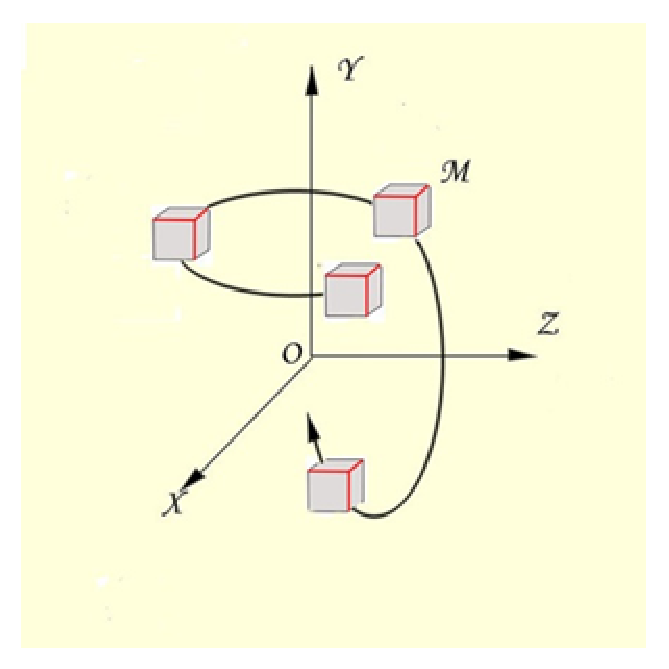
\includegraphics[width=0.3\textwidth]{img/img03.eps}
%\end{floatingfigure}

  Изучить движение тела - значит узнать, как изменяется его положение с
течением времени. Если это известно, то можно вычислить положение тела в любой
момент времени. В этом и состоит \textbf{основная задача механики - определять
положение тела в любой момент времени.} Так, астрономы, пользуясь законами
механики, могут вычислять положения небесных тел друг относительно друга и с
большой точностью предсказывать такие небесные явления, как затмения Солнца или
Луны.

  Чтобы решить основную задачу механики, нужно кратко и точно указать,
как движется тело, как изменяется его положение с течением времени. Другими
словами, надо найти математическое описание движения, установить связь между
величинами, характеризующими движение.

  Во многих случаях нет необходимости указывать положение каждой точки
движущегося тела. Одинаково движутся все точки чемодана, который мы поднимаем с
пола, кабины аттракциона <<колесо обозрения>> в парке, ступеньки эскалатора в
метрополитене и т. д. \textbf{Движение тела, при котором все его точки движутся
одинаково, называется поступательным.} При таком движении любая прямая, мысленно
проведенная в теле, остается параллельной самой себе.

  Если нас не интересует положение каждой точки твёрдого тела, например,
положение корабля в океане, то тело принимается за материальную точку.
\textbf{Тело, размерами которого в данных условиях движения можно пренебречь,
называют материальной точкой. }

\textbf{  Вращательным движением называется такое движение твёрдого тела, при
котором точки тела движутся в плоскостях, перпендикулярных неподвижной прямой,
называемой осью вращения, и описывают окружности, центры которых находятся на
этой оси. }


  Положение тела (точки) в пространстве определяется системой отчёта. В
систему отсчёта входят: тело отсчета, система координат, связанная с ним, и
прибор для измерения времени. Относительно выбранной системы отсчета и
рассматривается любое движение.

  Движение точки будет задано естественным способом, если будут известны

\begin{figure}[h]
\begin{center}
\includegraphics*[width=0.2\textwidth]{img/img04.eps}
\label{fig1}
\end{center}\end{figure}

\begin{enumerate}
  \item Траектория точки
  \item Зависимость изменения длины дуги от времени: $ОМ=S=f(t)$. Эта зависимость называется уравнением движения материальной точки
  \item Начало движения
  \item Начало отсчёта
  \item Направление отсчёта
\end{enumerate}

\begin{figure}[h]
\begin{center}
\includegraphics*[width=0.7\textwidth]{img/img02.eps}
\label{fig1}
\end{center}\end{figure}

  Положение точки в пространстве однозначно определяется радиус-вектором,
проведённым из некоторого неподвижного центра в данную точку $М$. Зависимость
изменения радиус-вектора от времени задаёт движение точки. Такой способ задания
называется векторным. Положение точки в пространстве в этом случае будет
определяться геометрическим местом концов векторов $r$, т.е. годографом её
радиус-вектора.

  При координатном способе задания движения (рис. \ref{fig5}), должны быть известны
зависимости, по которым можно определить координаты точки в пространстве
(декартова система координат).
\begin{wrapfigure}{l}{0.3\textwidth}
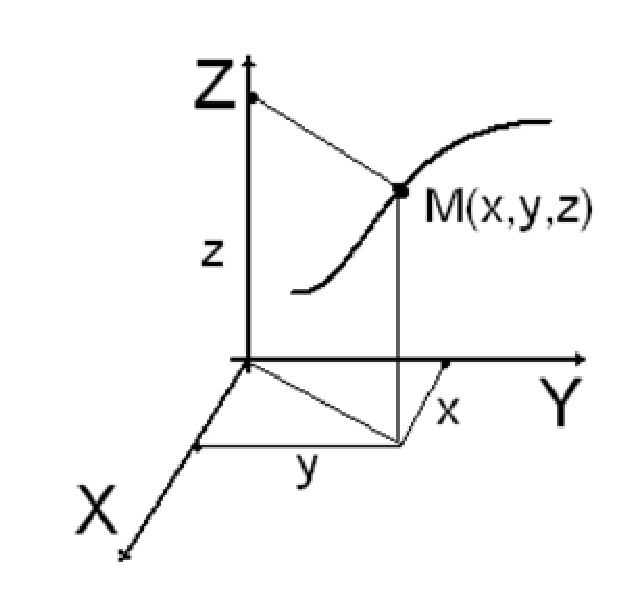
\includegraphics[width=0.3\textwidth]{img/img05.eps}
\caption{}
\label{fig5}
\end{wrapfigure}

\begin{gather*}
x=f_1(t)\\
y=f_2(t)\\
z=f_3(t)
\end{gather*}
\\
\\
\\

  Эти выражения выражают уравнение траектории в параметрической форме.
Решая их совместно и исключая параметр $t$, можно получить уравнение линии.
Зависимость $f(x,y,z)=0$ - это уравнение траектории.\\

\begin{wrapfigure}{l}{0.3\textwidth}
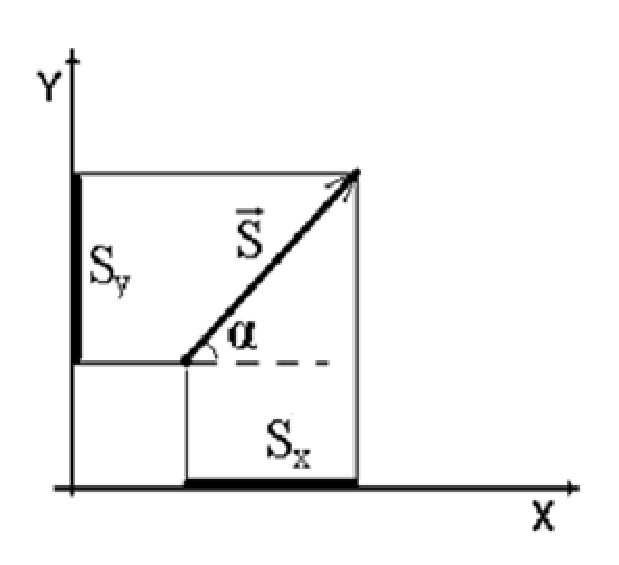
\includegraphics[width=0.3\textwidth]{img/img06.eps}
\caption{}
\label{fig6}
\end{wrapfigure}
  Перемещением тела (материальной точки) называют направленный отрезок
прямой, соединяющий начальное положение тела с его последующим положением.
Перемещение тела надо отличать от его траектории (линии вдоль которой
происходит движение тела). Необходимо также ввести понятие пути. Длиной пути $L$
называется сумма длин всех участков траектории, пройденной точкой за
рассматриваемый промежуток времени.

  Чтобы решить основную задачу механики необходимо знать перемещение. В
системе координат вектор задаётся проекциями. Проекция вектора на ось (рис. \ref{fig6}) равна
$S_x=S\cdot \cos\alpha, S_y=S\cdot \sin\alpha$. Модуль вектора можно найти по
теореме Пифагора, а угол между вектором и осью $Х$ равен $\alpha=\arcctg\ \frac{S_y}{S_x}$.
\\
\\

\begin{center}
   Вопросы
\end{center}

\begin{enumerate}
\item Что называется механическим движением тела?
\item В чём состоит основная задача механики?
\item Что такое поступательное движение тела?
\item Что такое материальная точка?
\item Что называется вращательным движением тела?
\item Что входит в систему отсчёта?
\item Как задаётся движение естественным способом?
\item В чём заключается векторный способ задания движения?
\item Что такое координатный способ задания движения?
\item Что такое перемещение тела?
\item Что такое траектория движения?
\item Что такое путь?
\end{enumerate}

\begin{center}
   Задачи
\end{center}
\begin{figure}
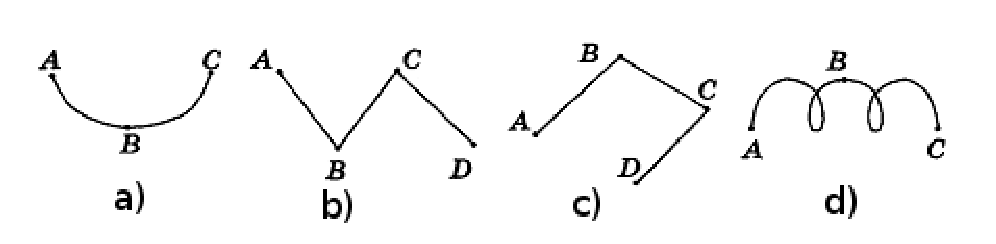
\includegraphics[width=0.8\textwidth]{img/ex15.eps}
\caption{Рисунки к задачам}
\label{ris}
\end{figure}

\begin{enumerate}
\item По заданной траектории движения тела найдите его перемещение (рис. \ref{ris}, a). Задачу решите графически.

\item Мальчик вышел из дому и прошел по прямым улицам сначала 2 квартала к востоку, а затем 2 квартала к северу (длина квартала 150 м). Определить путь и перемещение.
\item По заданной траектории движения тела найдите его перемещение (рис. \ref{ris}, b). Задачу решите графически.
\item Расстояние между пунктами А и В по прямой линии 6 км. Человек проходит это расстояние туда и обратно за 2 ч. Чему равны путь и перемещение человека за 2 и 1 ч?
\item По заданной траектории движения тела найдите его перемещение (рис. \ref{ris}, c). Задачу решите графически.
\item Мячик упал с высоты 2 м, отскочил от земли и был пойман на половине высоты. Укажите величину пути и численное значение перемещения мячика.
\item Велосипедист движется равномерно по окружности радиусом 100 м и делает один оборот за 2 мин. Определите путь и перемещение велосипедиста за 1 мин и за 2 мин.
\item Дорожка имеет форму прямоугольника, меньшая сторона которого равна 21 м, а большая - 28 м. Человек обходит всю дорожку за 1 мин. Определите перемещение и путь человека за 1 мин и за 0,5 мин.
\end{enumerate}

\begin{center}
   Домашнее задание
\end{center}

\begin{enumerate}
\item По заданной траектории движения тела найдите его перемещение (рис. \ref{ris}, d). Задачу решите графически.
\item Материальная точка движется по окружности с радиусом 2 м. Найдите путь и перемещение через 1/6 часть оборота, 1/4, 1/2 и полный оборот.
\item Автомобиль, двигаясь прямолинейно, проехал путь 10 м, затем сделал поворот, описав четверть окружности радиусом 10 м, и прошел далее по перпендикулярной улице еще 10 м. Сделайте в масштабе пояснительный чертеж, вычислите пройденный путь и найдите численное значение перемещения.
\end{enumerate}

\section{Равномерное движение}

  Мы рассмотрим сначала самый простой вид движения - прямолинейное
равномерное движение.

 Прямолинейное движение - это движение, при котором траектория тела (точки) -
прямая линия. Примером может служить движение автомобиля по участку дороги, на
котором нет подъемов, спусков, поворотов. А прямолинейным равномерным движением
называют такое движение, при котором тело (точка) за любые равные промежутки
времени совершает одинаковые перемещения. Для описания прямолинейного движения
удобно направить одну из координатных осей, например ось $X$, вдоль той прямой,
по которой движется тело.

  Как найти (вычислить) перемещение тела за какой-то промежуток времени
$t$. Для этого нужно знать перемещение тела за одну единицу времени. Скоростью
равномерного прямолинейного движения называют постоянную векторную величину,
равную отношению перемещения тела за любой промежуток времени к значению этого
промежутка $\vec{v}=\frac{\vec{S}}{t}$.

  Зная скорость $v$, мы найдем, и перемещение за любой промежуток времени $t$.
В проекциях это выглядит так:
\[
v_x=\frac{S_x}{t}\Rightarrow S_x=v_x t\ т.к.\ S_x=x-x_0,\ то\ x=x_0+v_xt
\]

 Выражение $x=x_0+v_xt$ называется уравнением движения для равномерного
прямолинейного движения.
\newpage
\section{Графическое представление движения}

\begin{wrapfigure}{l}{0.3\textwidth}
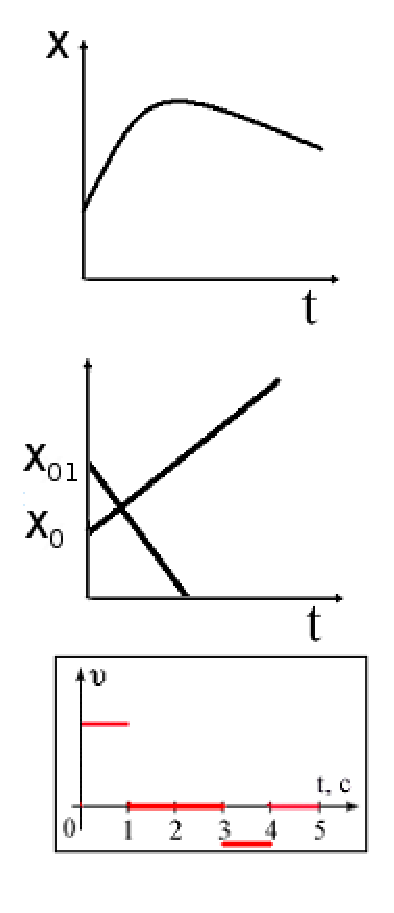
\includegraphics[width=0.3\textwidth]{img/img07.eps}
\caption{}
\label{fig7}
\end{wrapfigure}

  Формула $x=x_0+v_xt$ показывает, как с течением времени изменяется координата
 тела (точки) при прямолинейном равномерном движении. Она, как говорят,
описывает движение. Но описать движение тела можно и с помощью графика.
Допустим, что тело (точка) движется по некоторой прямой, вдоль горизонтальной
оси отложим в масштабе время, прошедшее с начала отсчета времени, а по
вертикальной оси (оси ординат) - тоже в определенном масштабе - значения
координаты тела, то полученный график показывает, как изменяется координата
тела со временем. Такой график называют графиком движения (не следует путать
с траекторией движения). График движения есть такое же описание движения, как
и формула. Для равномерного движения графиком зависимости координаты от
времени является прямая, выходящая из точки равной начальной координате тела.
Прямая наклонена под углом к оси ох, тангенс которого равен скорости
движения. Если скорость направлена вдоль оси ох, то прямая направлена вверх.
Если скорость направлена против оси - вниз.

 Наряду с графиками движения часто пользуются графиками скорости. Их получают,
откладывая по оси абсцисс время, а по оси ординат - проекции скорости тела.
Такие графики показывают, как изменяется скорость с течением. В случае
прямолинейного равномерного движения <<зависимость>> скорости от времени
состоит в том, что скорость со временем не изменяется. Поэтому график
скорости представляет собой прямую, параллельную оси времени.

  По графику скорости тоже можно определить перемещение тела за данный
промежуток времени, оно численно равно площади под графиком скорости.

\begin{center}
   Вопросы
\end{center}

\begin{enumerate}
\item Что называется прямолинейным равномерным движением?

\item Что такое скорость равномерного прямолинейного движения?

\item Что такое уравнение движения?

\item Что является графическим представлением движения?

\item Как определить перемещение по графику зависимости скорости от времени?
\end{enumerate}


\begin{center}
   Задачи
\end{center}
\begin{enumerate}
\item Сколько времени потребуется скорому поезду длиной 100 м. чтобы проехать
мост длиной 800 м, если скорость поезд равна 36 км/ч?

\item Один автомобиль, двигаясь равномерно со скоростью 15 м/с в течение 10 с,
совершил такое же перемещение, что и другой за 25 с. Какова скорость второго автомобиля?

\item Автомобиль, двигаясь со скоростью 54 км/ч, проехал половину пути до места
назначения за 2 ч. С какой скоростью он должен продолжать движение, чтобы
достигнуть цели и вернуться обратно за то же время?

\item Тело движется равномерно вдоль оси $X$. Модуль скорости равен 42 км/ч.
Найдите положение тела через 15 с после начала движения, если начальная
координата тела равнялась - 250 м. Чему равен путь, пройденный телом?

\item Движение точки на плоскости описывается уравнениями $х = 2 + 3t$, $у = 2t$.
Определить траекторию движения точки и построить ее на плоскости $ХОУ$.

\item Уравнения движения двух тел заданы выражениями $х_1 = 12 - 6t$ и
$х_2 = -9 + 3t$. Найдите время и координату места встречи тел.

\item Написать уравнения движения тел, графики которых даны на рисунке.

\item По графику скорости записать уравнение движения, $х_0=0$.


\item Даны уравнения движения: $х_1 = 3 +2t$ и $х_2 = 6 - t$. Найти начальную
координату, скорость, место и время встречи. Задачу решить аналитически и
графически.
\end{enumerate}

\begin{center}
   Домашнее задание
\end{center}
\begin{enumerate}
\item По озеру буксир тянет баржу со скоростью 12 км/ч. Длина буксира с баржей
100 м. Сколько времени буксир с баржой будет проходить мимо теплохода, стоящего
у пристани, если длина теплохода 50 м?

\item Поезд длиной 200 м, двигаясь равномерно, прошел мост за 1 мин. Какова
скорость поезда, если длина моста 300 м?

\item Поезд длиной 100 м движется по мосту равномерно со скоростью 72 км/ч. За
сколько минут он пройдет мост, если его длина 850 м?

\item Вдоль оси Х движутся две точки: первая - по закону $х_1 = 6 + 2t$, а
 вторая по закону $х_2 = -1 + 5t$. В какой момент времени они встретятся?

\item Тело движется против оси ОХ. Модуль скорости равен 36 км/ч. Начальная
координата равна 10 м. Найдите положение тела через 6 с. Чему равен путь, пройденный телом?

\item Написать уравнения движения тел, графики которых даны на рисунке.

\item По графику скорости записать уравнение движения. $х_0=0$.

\item Даны уравнения движения: $х_1= 1+1,5t$ и $х_2= 6- 2t$. Найти начальную
 координату, скорость, место и время встречи. Задачу решить аналитически и
 графически.

\item Даны уравнения движения: $х_1 = 10(2-t)$ и $x_2=2(-3+2t)$. Найти
начальную координату, скорость, место и время встречи. Задачу решить
аналитически и графически.

\item Даны уравнения движения: $х_1 = 1,5(2-t)$ и $x_2 = 1,2(t -2)$. Найти
начальную координату, скорость, место и время встречи. Задачу решить
аналитически и графически.
\end{enumerate}

\section{Относительность движения}

\begin{wrapfigure}{l}{0.3\textwidth}
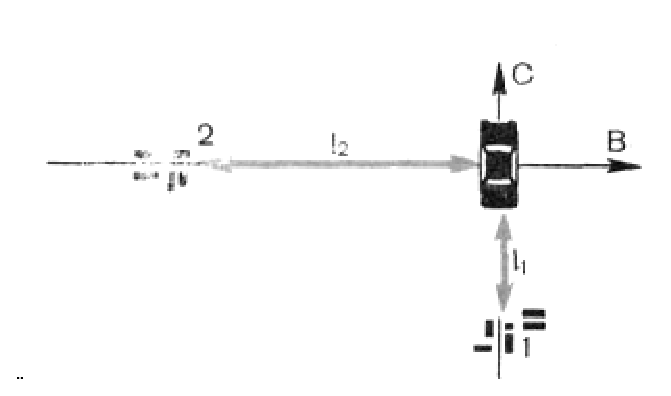
\includegraphics[width=0.3\textwidth]{img/img_08.eps}
\caption{}
\label{fig8}
\end{wrapfigure}

 Положение тела в пространстве всегда задается относительно какого-то другого
тела - тела отсчета. С этим телом связывают систему координат, и положение тела
задается его координатами. Но за тело отсчета можно выбрать любое тело и с
каждым из них связать систему координат. Тогда положение одного и того же тела
можно рассматривать относительно разных систем отсчета.

  Координаты одного и того же тела относительно разных тел отсчета могут
оказаться различными. Например, положение автомобиля на дороге (рис. \ref{fig8}) можно
задать, указав, что он находится на расстоянии $l_1$ к северу от населенного
пункта 1. Но можно сказать, что автомобиль расположен на расстоянии $l_2$ к
востоку от населенного пункта 2. Это и значит, что положение тела относительно:
оно различно относительно разных систем координат.

  Относительно не только положение тела. Относительно и его движение. В чем
состоит относительность движения? Рассмотрим движение одного и того же тела
относительно двух разных систем отсчета, движущихся одна относительно другой
прямолинейно и равномерно. Одну из них мы будем условно считать неподвижной.
Другая движется относительно нее прямолинейно и равномерно.

  Вот простой пример. Лодка пересекает реку перпендикулярно течению, двигаясь с
 некоторой скоростью относительно воды. Вода в реке движется относительно
берега со скоростью течения реки. Представим себе, что за движением человека
следят два наблюдателя: один неподвижный, расположился на берегу в точке $О$,
другой - на плоту, плывущем по течению (со скоростью течения реки). Оба
наблюдателя измеряют перемещение человека и время, затраченное на него.
Относительно воды плот неподвижен, а по отношению к берегу, он движется со
скоростью течения реки. Проведем мысленно через точку $О$ систему координат
$ХОУ$. Ось $X$ направим вдоль берега, ось $У$ - перпендикулярно течению реки.
Это неподвижная система отсчета. Другую систему координат $Х_1 О_1 У_1$
свяжем с плотом. Оси $X_1$ и $У_1$ параллельны осям X и У. Это - подвижная
система координат. Как движется человек относительно наших двух систем?

  Наблюдатель на плоту, двигаясь вместе со <<своей>> системой координат по
течению, видит, что человек удаляется от него к противоположному берегу все
время перпендикулярно течению со скоростью $v_1$ , и совершает перемещение
$S_1$.

  Совсем другим представится движение лодки неподвижному наблюдателю на
берегу. Относительно <<его>> системы координат человек за то же время $t$
совершил перемещение $S$. За это же время подвижная система отсчета вместе с
плотом совершила перемещение $S_2$. Схематически перемещения лодки показаны
на рисунке. Из рисунков видно, что перемещение S лодки относительно
неподвижной системы координат связано с перемещениями $S_1$ и $S_2$ формулой:

\[\vec{S}=\vec{S_1}+\vec{S_2}\]

  Скорость $v$ лодки относительно неподвижной системы координат мы получим,
разделив перемещение $S$ на время $t$: или
$\frac{\vec{S}}{t}=\frac{\vec{S_1}}{t}+\frac{\vec{S_2}}{t}$, это формула
сложения скоростей.

\textbf{  Скорость тела относительно неподвижной системы координат равна
геометрической сумме скорости тела относительно подвижной системы координат и
скорости подвижной системы относительно неподвижной.}

  Мы видим, что и перемещение и скорость тела относительно разных систем
отсчета различны. Различны и траектории движения ($СС_1$ - относительно
подвижной системы и $ОС_1$ - относительно неподвижной). В этом и состоит
относительность движения.

  В нашем примере мы считали неподвижной систему координат, связанную с
берегом. Но мы могли бы условиться считать неподвижной систему координат,
связанную с плотом. Тогда подвижным оказался бы берег и связанная с ним система
координат, и мы рассматривали бы движение берега относительно плота и лодки.
Формулы сложения перемещений и скоростей остались бы такими же. Мы уже и раньше
говорили, что относительно не только движение, относителен и покой.

\begin{center}
   Вопросы
\end{center}
\begin{enumerate}
\item Какими величинами определяется положение тел в пространстве? Сколько таких величин?
\item Что такое система отсчёта?
\item Может ли координата быть отрицательной величиной?
\item Может ли изменение координаты быть отрицательной величиной?
\item Наблюдения показали: за время матча футболист пробежал 12 км. Что это - перемещение или путь?
\item Штурман, определяя утром положение корабля, обнаружил, что корабль находится в точке, расположенной на 100км к северу от пункта, в котором находился накануне вечером. Что это - перемещение или путь?
\item Автомобиль движется к востоку со скоростью 40км/ч. Другой автомобиль движется к югу со скоростью 40км/ч. Можно ли сказать, что скорости автомобилей равны?
\item Можно ли зная начальное положение тела и его путь, найти конечное положение тела?
\item Как связать скорость тела с изменением его положения при движении?
\item В   чем   состоит   относительность   движения?
\item Как   в   примере   с   лодкой   движутся вода и берег относительно лодки?
\item Комбайн,   убирающий   в   поле    хлеб, движется относительно земли со скоростью 2,5 км/ч и, не останавливаясь, ссыпает зерно в автомашину. Относительно какого тела отсчета автомашина движется и относительно какого покоится?
\end{enumerate}

\begin{center}
   Задачи
\end{center}
\begin{enumerate}
\item{ По дороге навстречу друг другу движутся два автомобиля: один со скоростью
60 км/ч, другой - 90 км/ч. У заправочной станции автомобили встретились и
продолжили свой путь. Определите положение каждого автомобиля через 30 мин
после встречи и расстояние между ними в этот момент.

 \textbf{Решение.} За начало координат примем заправочную станцию, а время будем
отсчитывать от момента встречи автомобилей. Координатную ось $X$ направим по
направлению движения первого автомобиля. Тогда координаты автомобилей через
$0,5 ч$ после встречи можно вычислить по формулам: $х = х_0 + v_xt$.
Начальные координаты $х_{01}$ и $х_{02}$ у обоих автомобилей равны нулю.
Поэтому $х_1 = 60\cdot 0,5 = 30 (км)$, $х_2 = -90\cdot0,5 = 45 (км)$.
Расстояние между автомобилями равно разности их координат
$l = х_1 - х_2 = 30-(-45) = 75 (км)$
}

 \item{ Два автомобиля движутся по взаимно перпендикулярным дорогам (рис. \ref{fig9}), но
направлению к перекрестку. В некоторый момент времени первый автомобиль,
скорость $v_1$ которого равна 27 км/ч, находится на расстоянии $l_1$ = 300 м
от перекрестка. Второй в тот же момент времени находится на расстоянии $l_2$
= 450 м от перекрестка. С какой скоростью $v_2$ движется второй автомобиль,
если он достигает перекрестка через $t= 5с$ после первого?

\textbf{Решение.} За начало отсчета координат примем перекресток дорог, а отсчет
времени начнем с момента, когда автомобили находились на расстояниях $l_1$ и $l_2$ от
перекрестка. Оси координат направим вдоль дорог. Первый автомобиль движется
вдоль оси $X$, второй - противоположно направлению оси $У$. Поэтому при движении
первого автомобиля изменяется со временем только координата $х$. Ее найдем по
формуле: \[x=x_0+v_1t, 0=-l_1+v_1t_1\]

  Для второго автомобиля $y = y_0 - v_2(t_1 + t)$, $0 = l_2 - v_2(t_1 + t)$,
решая совместно эти два уравнения, получим:
\[
v_2=\frac{l_2}{\frac{l_1}{v_1}+t}=
\frac{l_2\cdot v_2}{l_1+v_1t}=
\frac{450\cdot 7,5}{300+37,5}
=10 \frac{м}{с}
\]
}
\end{enumerate}

\begin{figure}
\begin{center}
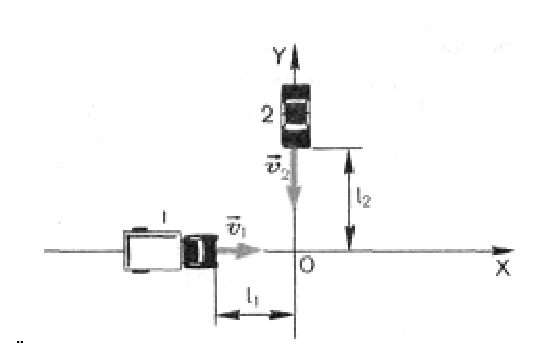
\includegraphics[width=0.3\textwidth]{img/img_09.eps}
\caption{}
\end{center}
\label{fig9}
\end{figure}

\begin{center}
   Домашнее задание
\end{center}
\begin{enumerate}
\item Застигнутый грозой путник увидел вспышку молнии, а через 10 с до него донеслись раскаты грома. На каком расстоянии от него произошел грозовой разряд, если скорость звука в воздухе равна 340 м/с?
\item Двигатель самолета сообщает ему скорость относительно воздуха, равную 900 км/ч. С какой скоростью движется самолет относительно Земли при попутном ветре, скорость которого равна 50 км/ч; при таком же встречном ветре?
\item Скорость первого автомобиля относительно второго 100 км/ч. Определите скорость второго автомобиля относительно Земли, если скорость первого относительно Земли 60 км/ч. Автомобили движутся навстречу друг другу.
\item Скорость течения реки 1 км/ч. Моторная лодка идет против течения со скоростью 10 км/ч (относительно земли). С какой скоростью она будет двигаться по течению (относительно земли и относительно воды)?
\item Велосипедист едет со скоростью 30 км/ч. Скорость ветра 3 м/с. Определите скорость ветра относительно велосипедиста, если: а) ветер встречный; б) ветер боковой.
\end{enumerate}


\section{Неравномерное движение. Средняя скорость}

 В некоторых случаях, когда имеют дело с неравномерным движением, пользуются
средней скоростью. Ее получают, разделив перемещение тела $S$ на время, в течение
которого оно совершено:
\[\vec{v}_{ср}=\frac{\vec{S}}{t}\]

 Если, например, поезд, двигаясь по прямой, проходит 600 км за 10 ч, то это
значит, что в среднем он за каждый час проходит 60 км. Но ясно, что какую-то
часть времени поезд вовсе не двигался, а стоял на остановке; трогаясь со
станции, поезд увеличивал свою скорость, приближаясь к ней - уменьшал ее. Все
это при определении средней скорости мы не принимаем во внимание и считаем, что
поезд каждый час проходил по 60 км, каждые полчаса - по 30 км и т.д. Пользуясь
формулой, мы, как бы считаем, что поезд двигался равномерно со скоростью 60
км/ч, хотя, быть может, за все эти 10 ч не было ни одного такого часа, за
который поезд прошел бы именно 60 км. Знание средней скорости позволяет найти
перемещение по формуле
\[\vec{S}=\vec{v}_{ср}\cdot t\]

 Но надо помнить, что эта формула дает верный результат только для того участка
траектории, для которого определена средняя скорость. Если, пользуясь значением
средней скорости в 60 км/ч, вычислять перемещение поезда не за 10 ч, а за 2, 4
или 5 ч, то мы получим неверный результат. Средняя скорость за время 10 ч не
равна средним скоростям за 2, 4 или 5 ч.

Таким образом, средняя скорость, вообще говоря, не позволяет вычислять
перемещение, а значит, и координаты в любой момент времени.

\begin{center}
   Задачи
\end{center}
\begin{enumerate}
\item На горизонтальном участке пути автомобиль ехал со скоростью 72 км/ч в
течение 20 мин, а затем проехал подъем со скоростью 36 км/ч за 40 мин. Чему
равна средняя скорость на всем пути?

\item Автомобиль проехал первую половину пути со скоростью 40 км/ч, а вторую
- со скоростью 60 км/ч. Определить среднюю скорость его движения.

\item Из одного пункта в другой мотоциклист двигался со скоростью 70 км/ч,
обратный путь им был пройден со скоростью 15 м/с. Определите среднюю скорость
мотоциклиста за все время движения.

\item Пешеход часть пути прошел со скоростью 4 км/ч, затратив на это 2/3 времени
 своего движения. За оставшуюся треть времени он прошел остальной путь со
  скоростью 5 км/ч. Определите среднюю скорость.

\item Скорость поезда между двумя пунктами равна 80 км/ч, средняя скорость на
всем пути 60 км/ч, причем остановки занимают время 1 час. Найти расстояние между
 этими пунктами.

\item Автомобиль проехал половину пути со скоростью 60 км/ч, оставшуюся часть
пути он половину времени шел со скоростью 15 км/ч, а последний участок - со
скоростью 45 км/ч. Найти среднюю скорость автомобиля на всем пути.

\item Велосипедист ехал из одного города в другой. Половину пути он проехал со
скоростью 12 км/ч. Далее половину оставшегося времени он ехал со скоростью
6 км/ч, а затем до конца пути шел пешком со скоростью 4 км/ч. Определить среднюю
скорость движения велосипедиста на всем пути.
\end{enumerate}

\begin{center}
   Домашнее задание
\end{center}
\begin{enumerate}
\item Двигаясь по шоссе, велосипедист проехал 90 м со скоростью 15 м/с, а затем
по плохой дороге 40 м со скоростью 10 м/с. С какой средней скоростью он проехал
весь путь?

\item Велосипедист проехал первую половину пути со скоростью 15 км/ч, а вторую
половину пути со скоростью $v_2$. Как велика эта скорость, если известно, что
средняя скорость его движения на всем пути равна 10 км/ч?

\item Скорость поезда на подъеме 20 км/ч, а на спуске - 80 км/ч. Определите
среднюю скорость на всем участке пути, если спуск в два раза длиннее подъёма?

\item На первой половине пути автобус двигался со скоростью, в 8 раз большей,
чем на второй. Средняя скорость автобуса на всем пути 16 км/ч. Определить
скорость автобуса на обеих половинах пути.
\end{enumerate}

\section{Равноускоренное прямолинейное движение. Аналитическое и графическое
описание равноускоренного прямолинейного движения}

  Средняя скорость, не позволяет вычислять перемещение, а значит, и
координаты в любой момент времени. Для вычисления положения тела в любой момент
времени Необходимо знать мгновенную скорость.

\begin{figure}
\begin{center}
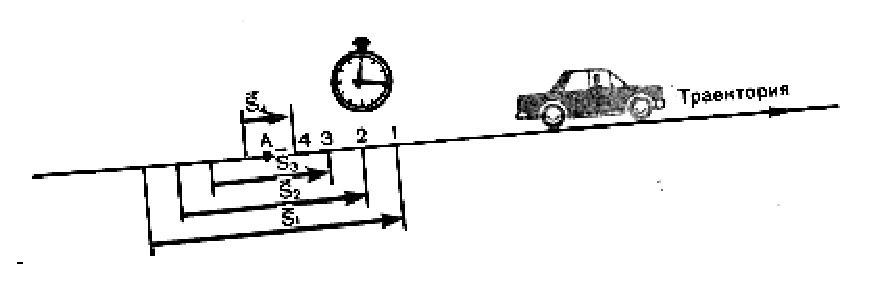
\includegraphics[width=0.3\textwidth]{img/img_10.eps}
\caption{}
\end{center}
\label{fig10}
\end{figure}


  Всякое движущееся тело обладает скоростью. С другой стороны, при своем
движении по траектории тело проходит через все ее точки. А таких точек
бесконечно много. Через каждую из них тело проходит в определенный момент
времени. Таких моментов времени тоже бесконечно много. Выходит поэтому, что в
каждый момент времени и в каждой точке траектории тело обладает какой-то
скоростью. Вот эта скорость и называется мгновенной. Мгновенной скоростью
тела называется скорость тела в данный момент времени или в данной точке
траектории.

  При прямолинейном равномерном движении скорость тела равна отношению
его перемещения к промежутку времени, за который это перемещение совершено.

  Допустим, что некоторое тело (как всегда, мы имеем в виду определенную
точку тела) движется прямолинейно, но не равномерно. Нас интересует мгновенная
 скорость, например, в точке $А$ его траектории (рис. \ref{fig10}). Выделим небольшой
участок $S_1$ на этой траектории, включающий точку $А$. Малое перемещение тела
на этом участке обозначим через $s_1$, а малый промежуток времени, в течение
которого оно совершено, через $t_1$. Разделив $S_1$ на $t_1$, мы получим
среднюю скорость на этом участке; это именно средняя скорость, потому что
скорость непрерывно изменяется, и в разных местах участка она разная.
Уменьшим теперь длину участка. Выберем участок 2 (см. рис. 37), тоже
включающий точку $А$. Перемещение теперь равно $S_2$ ($S_2<S_1$), и совершает
его тело за меньший промежуток времени $t_2$. На этом участке скорость
успевает измениться на меньшую величину. Но отношение дает нам и теперь
среднюю скорость на этом меньшем участке. Еще меньше изменение скорости на
протяжении участка 3 (также включающего в себя точку $A$). Будем продолжать
уменьшать промежуток времени, за который мы рассматриваем перемещение тела.
Вместе с ним будет уменьшаться и перемещение. В конце концов, промежуток
времени станет так мал, что можно будет пренебречь изменением скорости за это
время (движение станет как бы равномерным). Участок траектории, пройденный за
этот, совсем уже малый, промежуток времени как бы стянется в точку $А$, а
промежуток времени - в момент времени. Тогда-то средняя скорость и станет
мгновенной скоростью тела в точке $А$.

  Мгновенная скорость, или скорость в данной точке, равна пределу
отношения перемещения на участке траектории, примыкающем к этой точке, к
промежутку времени, в течение которого это перемещение совершается, при
$\Delta t$ стремящемся к нулю.

\[\vec{v}=\lim_{\Delta t\to\infty}\frac{\Delta\vec{S}}{\Delta t}=
\frac{d\vec{S}}{dt}
\]

  Мгновенная скорость - это векторная величина. Вектор мгновенной
скорости направлен по касательной к траектории движения в данной точке. В
дальнейшем, говоря о скорости неравномерного движения, мы будем иметь в виду
именно мгновенную скорость.

  О мгновенной скорости можно говорить и в случае равномерного движения.
Разница только в том, что при равномерном движении мгновенная скорость в любой
точке и в любой момент времени одна и та же. При неравномерном же движении она
в разных точках и в различные моменты времени различна.

\section{Ускорение. Равнопеременное движение}

  При неравномерном движении мгновенная скорость тела непрерывно
изменяется от точки к точке, от одного момента времени до другого. Как же
вычисляется мгновенная скорость?

  Мы видели раньше, что для вычисления координаты тела в любой момент
времени нужно знать, как быстро она изменяется, т. е. каково ее изменение за
единицу времени. Быстрота изменения координаты равна, как мы видели, проекции
скорости на соответствующую координатную ось. Точно так же для вычисления
скорости в любой момент времени нужно знать, как быстро изменяется скорость,
насколько она изменяется за единицу времени. Быстрота изменения скорости
называется ускорением.

\[Мгновенное\ ускорение\ равно\ \vec{a}=\lim_{\Delta t\to\infty}\frac{\Delta\vec{v}}{\Delta t}
\ или \ \vec{a}=\frac{d\vec{v}}{dt}
\]

  Для простоты мы будем рассматривать такое неравномерное движение, при
котором скорость тела за каждую единицу времени и вообще за любые равные
промежутки времени изменяется одинаково. Движение тела, при котором его
скорость за любые равные промежутки времени изменяется одинаково, называется
равнопеременным движением.

 Если в некоторый начальный момент времени скорость тела равна $v_0$, а через
промежуток времени t она оказывается равной $v$, то ускорение найдём по формуле:
\[\vec{a}=\frac{\vec{v}-\vec{v}_0}{t}\]


  Ускорением тела при его равноускоренном движении называется величина,
равная отношению изменения скорости к промежутку времени, в течение которого
это изменение произошло.

  Ускорение - величина векторная.

  Если ускорение тела по модулю велико, это значит, что тело быстро
набирает скорость (когда оно разгоняется) или быстро теряет ее (при торможении).

  За единицу ускорения в СИ принимается ускорение такого равноускоренного
движения, при котором за 1 с скорость тела изменяется на 1 м/с. Следовательно,
в СИ ускорение выражается в метрах в секунду за секунду или в метрах на секунду
в квадрате ($м/с^2$).

 Проекции скорости и ускорения. Мы уже говорили, что при вычислениях нужно
пользоваться формулами, в которые входят не векторы, а их проекции на оси
координат.

 При прямолинейном движении
\[a_x=\frac{v_x-v_{x0}}{t},\]
\[\vec{v}=\vec{v}_0+\vec{a}t,\ v_x=v_{x0}+a_{x}t\]

 При ускорении, вектор $\vec{a}$ сонаправлен вектору $\vec{v}$: равноускоренное
движение. При торможении вектор $\vec{a}$ направлен противоположно вектору
$\vec{v}$: равнозамедленное движение.

 Если скорость тела с течением времени уменьшается, (тело тормозит), то в
какой-то момент времени скорость тела может стать равной нулю. Как оно
движется после этого? Ясно, что, когда какая-либо величина, изменяясь,
проходит через значение нуль, она изменяет свой знак на противоположный. В
нашем случае изменяет знак скорость. Это значит, что после того, как скорость
тела станет равной нулю, оно начнет двигаться в противоположном направлении.


\section{Перемещение при прямолинейном равноускоренном движении}

\begin{wrapfigure}{l}{0.2\textwidth}
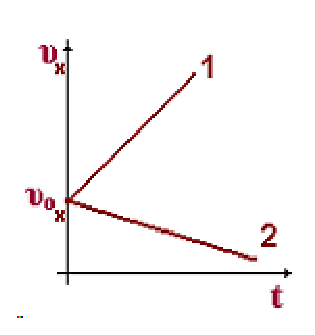
\includegraphics[width=0.2\textwidth]{img/img11.eps}
\caption{}
\label{fig11}
\end{wrapfigure}
  Формулу для вычисления перемещения проще всего получить графическим
методом. При равноускоренном движении тела вдоль оси X скорость изменяется со
временем согласно формуле \[{v}_x={v}_{x0}+a_{x}t\]

Так как время в эту формулу входит в первой степени,
то график для проекции скорости в зависимости от времени представляет собой
прямую, как это показано на рисунке \ref{fig11}. Прямая 1 на этом рисунке соответствует
движению с положительной проекцией ускорения (скорость растет), прямая 2 -
движению с отрицательной проекцией ускорения (скорость убывает). Оба графика
относятся к случаю, когда в момент времени $t_0 = 0$, тело имеет некоторую
начальную скорость $v_0$.
\begin{wrapfigure}{l}{0.2\textwidth}
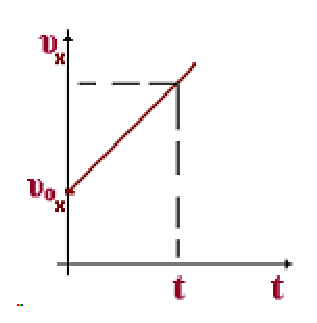
\includegraphics[width=0.2\textwidth]{img/img12.eps}
\caption{}
\label{fig12}
\end{wrapfigure}
Перемещение выражается площадью, заключённой под
графиком. Перемещение за все время $t$ численно равно площади трапеции. Площадь
же трапеции, как известно из геометрии, равна произведению полусуммы ее
оснований на высоту
\[S_x=\frac{v_{x0}+v_x}{2}\cdot t,\  но\ отсюда \]
\[S_x=v_{x0}+\frac{a_x t^2}{2}\]

  Таким образом, мы видим, что при равноускоренном движении перемещение
растет со временем не так, как при равномерном движении: теперь в формулу
входит квадрат времени. Это значит, что перемещение со временем растет быстрее,
чем при равномерном движении и графиком зависимости координаты от времени
является парабола.

\begin{wrapfigure}{l}{0.2\textwidth}
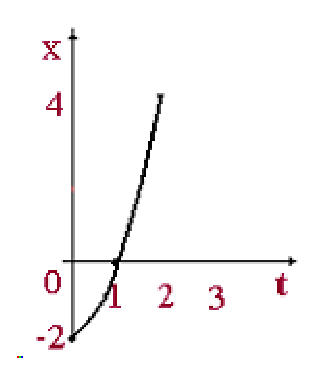
\includegraphics[width=0.2\textwidth]{img/eps13.eps}
\caption{}
\label{fig13}
\end{wrapfigure}


  Как зависит от времени координата тела? Теперь легко получить и формулу
для вычисления координаты $х$ в любой момент времени для тела, движущегося
равноускоренно: $S_x=x-x_0$, отсюда $x=x_0+S_x$. Поэтому
\[x=x_0+v_{x0}t+\frac{a_x t^2}{2}\]

  Для вычисления перемещения можно получить и другую полезную формулу, в
которую время не входит.
\begin{figure}
\begin{center}
  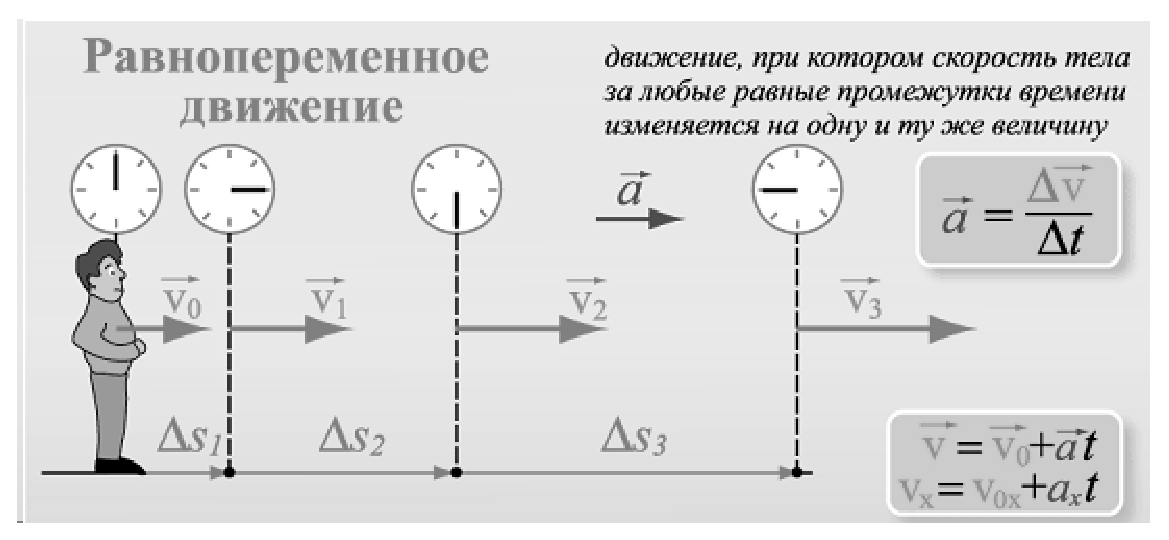
\includegraphics[width=0.8\textwidth]{img/img14.eps}\\
  \caption{}\label{img14}
\end{center}
\end{figure}
Из выражения $v_x=v_{x0}+a_x$ получим выражение для
$t$ и подставим его в формулу для перемещения, приведенную выше. Тогда
получаем:
\[S_x=\frac{v_x^2-v_{x0}^2}{2a_x}\]


  Эти формулы позволяют найти перемещение тела, если известны ускорение,
а также начальная и конечная скорости движения.

  Формулу перемещения можно получить, решая дифференциальное уравнение.
Пусть тело движется с постоянным ускорением $\vec{a}$.

По определению $\vec{a}=\frac{d\vec{v}}{dt}\to\vec{a}dt=d\vec{v}$,
интегрируя обе части уравнения, получим
\[\int\limits_{0}^{t}\vec{a}dt=\int\limits_{v_0}^{v}d\vec{v}\to\vec{v}=
\vec{v}_0+\vec{a}t,\ или\ \frac{d\vec{S}}{dt}=\vec{v}_0+\vec{a}t
\]
Умножим обе части уравнения на dt:
\[d\vec{S}=\vec{v}_0\cdot dt+\vec{a}t\cdot dt,\]
интегрируя ещё раз, получим
\[
\int\limits_{0}^{S}d\vec{S}=\int\limits_{0}^{t}\vec{v}_0dt+
\int\limits_{0}^{t}\vec{a}tdt\to\vec{S}-0=
\vec{v}_0\cdot t-\vec{v}_0\cdot 0+\frac{\vec{a}\cdot{t^2}}{2}-
\frac{\vec{a}\cdot{0^2}}{2}\to
\vec{S}=\vec{v}_0t\vec{+}\frac{\vec{a}t^2}{2}
\]

\begin{center}
   Вопросы
\end{center}
\begin{enumerate}
\item Что  такое  ускорение   и   для   чего  его нужно знать?
\item При любом неравномерном движении изменяется   скорость.   Как   ускорение   характеризует это изменение?
\item Чем   отличается   <<замедленное>>   прямолинейное    движение    от    <<ускоренного>>?
\item Что     такое     равноускоренное     движение?
\item Может ли  тело двигаться  с большой скоростью, но с малым ускорением?
\item Как направлен  вектор ускорения  при прямолинейном неравномерном движении?
\item Скорость - векторная величина, и изменяться может как модуль скорости, так и  направление вектора скорости. Что именно изменяется при прямолинейном  равноускоренном движении?
\item Может ли скорость движения  тела быть равной  нулю, а ускорение не равно нулю?
\item Чем отличается график скорости равномерного прямолинейного движения от графика скорости равноускоренного движения?
\item Как   по   графику   проекции   скорости равноускоренного      движения      определяют проекцию перемещения тела?
\item Чем различаются зависимости перемещения от времени при равномерном и равноускоренном движениях?
\end{enumerate}
\begin{center}
   Решение задач
\end{center}
\begin{figure}
\begin{center}
%  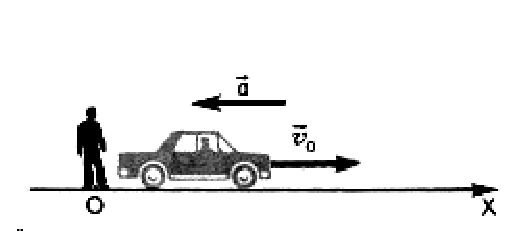
\includegraphics[width=0.2\textwidth]{img/img15.eps}
  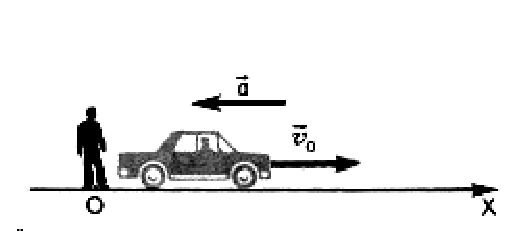
\includegraphics[width=0.35\textwidth]{img/img15.eps}\\
\end{center}
  \caption{}\label{img1516}
\end{figure}
\begin{enumerate}

\item { Автомобиль проезжает мимо наблюдателя, двигаясь со скоростью 10 м/с. В этот
момент водитель нажимает на тормоз и автомобиль начинает двигаться с
ускорением, по модулю равным $1\ м/с^2$. Сколько времени пройдет до остановки
автомобиля?

  \textbf{Решение}. Выберем за начало отсчета координаты место нахождения
наблюдателя, а координатную ось направим в сторону движения автомобиля (рис.
\ref{img1516}). Обозначим скорость автомобиля в момент, когда он проходит мимо
наблюдателя, через $v_0$, а его ускорение после включения тормоза через $а$.
Воспользуемся формулой $v_x=v_{x0}+a_xt$. В момент остановки $v_x= 0$.
Ускорение при торможении направлено против скорости, т.е. отрицательно.
Следовательно, $0 = v_{x0}-а_{х}t $ или $t = \frac{v_{x0}}{a_x}$. Подставив в
это выражение значения $v_{x0}$ и $а_x$, получим $t = 10/1=10(c)$.
}

\item {
  Тело движется прямолинейно с уменьшающейся скоростью. Ускорение $а$ постоянно
и по модулю равно $4\ м/с^2$. В некоторый момент времени модуль скорости тела
$v_0 =20\ м/с$. Найдите скорость тела через $t_1=4с$ и $t_2=8с$ после этого
момента.

\textbf{Решение.} Направим координатную ось $X$ по направлению вектора скорости
$v_0$. Тогда проекция $v_{x0}$ положительна и равна модулю вектора $v_0$ . А так как
скорость тела уменьшается, то проекция ускорения $a_x$ отрицательна и равна $а_x=-а$.
Чтобы найти проекцию скорости в указанные в задаче моменты времени
применим формулу $v_x=v_{x0}+a_xt$. Отсюда для момента времени $t_1$ найдем:
\[v_1=20-4\cdot 4 = 4(м/c),\]
\[v_2=20-4\cdot 8 = -12(м/c)\]

  Знак <<минус>> означает, что к исходу 8-й секунды тело двигалось в
направлении, противоположном начальному. Очевидно, что перед тем, как начать
движение в обратном направлении, тело должно было остановиться. В какой
момент времени $t$ это произошло? Проекция $v$ равна нулю, когда
$v_{x0}=-a_{x}t$. Отсюда $t'=-20/-4=5(с)$.

 Направление движения изменилось на обратное через 5 с после того момента, когда
скорость тела была равна 20 м/с. Двигаться так, как описано в этой задаче,
могло бы, например, тело, которое толкнули вверх по наклонной плоскости.
}
\item {
 Водитель автомобиля, движущегося со скоростью 72 км/ч, увидев красный свет
светофора, нажал на тормоз. После этого скорость автомобиля стала уменьшаться
на 5 м/с каждую секунду. Найдите расстояния, которые автомобиль проходит в
первые 2 с после начала торможения и до полной его остановки.

 \textbf{Решение}. Координатную ось $X$ направим по направлению движения
автомобиля (рис. \ref{img1516}), а за начало отсчета координаты примем то место на дороге,
где началось торможение. Начало отсчета времени отнесем к моменту, когда
водитель нажал на тормоз. Начальная скорость $v_0$ автомобиля сонаправлена с осью
$X$, а ускорение направлено в противоположную сторону, так что проекция начальной
скорости $v_{x0}$ положительна, а проекция ускорения $a_x$ - отрицательна. Расстояния,
пройденные автомобилем,- это проекции перемещения $S_x$,
\[
S_2=v_{x0}t-\frac{a_x t^2}{2}\to S_2=20\cdot 2-\frac{5\cdot 2^2}{2}=30(м)
\]
\[
S_{полное}=\frac{v_x^2-v_{x0}^2}{-2a_x}\to S_{полное}=\frac{-v_{x0}^2}{-2a_x}\to
S_{полное}=\frac{-20^2}{-2\cdot 5}=40(м)
\]
}
\item {
Определите перемещение тела, график проекции скорости которого показан на
рисунке.

 \textbf{Решение:} Перемещение равно площади под графиком скорости. За первые
две секунды тело двигалось вдоль оси $Х$, а за третью секунду - против оси $Х$.
Поэтому перемещение тела равно разности площадей треугольников.
\[
S = S_{042}-S_{23(-2)},\ S = 2\cdot 4/2-1\cdot 2/2= 3(м).
\]

}
\end{enumerate}

\begin{center}
   Задачи
\end{center}
\begin{enumerate}
\item Через 20 с после начала движения спидометр автомобиля показал скорость движения 72 км/ч. С каким ускорением двигался автомобиль?
\item За какое время автомобиль, двигаясь из состояния покоя с ускорением $0,4\ м/с^2$, пройдет 30 м?
\item Какую скорость будет иметь тело через 20 с от начала движения, если ускорение его движения равно $360\ м/мин^2$?
\item Поезд метро, отходя от станции, может развить скорость 36 км/ч за 20 с. Определить ускорение его движения. Какой путь при этом поезд проходит?
\item Велосипедист, движущийся со скоростью 2 м/с, начинает спускаться с горы с ускорением $0,6\ м/с^2$. Найдите длину горы, если спуск занял 10 с.
\item Начав торможение с ускорением $0,3\ м/с^2$, поезд прошел до остановки 250 м. Какова была его скорость перед началом торможения?
\item Пуля, летящая со скоростью 300м/с, ударяет в земляной вал и проникает в него на глубину 56 см. Сколько времени двигалась она внутри вала? С каким ускорением? Какова была ее скорость на глубине 20 см?
\item Тело, имея начальную скорость 3 м/с, двигалось равноускоренно и приобрело, пройдя некоторое расстояние, скорость 12 м/с. Какова была скорость тела на половине этого расстояния?
\item По наклонной доске пустили катиться снизу вверх шарик. На расстоянии 50 см от начала пути шарик побывал дважды: через 2 с и через 4 с после начала движения. Определите начальную скорость и ускорение.
\item Тело, имея начальную скорость 2 м/с, прошло за пятую секунду путь, равный 8 м. Определить ускорение и путь, пройденный телом за 10 с.
\end{enumerate}

\begin{center}
   Домашнее задание
\end{center}
\begin{enumerate}
\item Троллейбус,    трогаясь   с   места,    движется   с   постоянным   ускорением   $1,5   м/с^2$ . Через    какое   время    он    приобретает   скорость 54 км/ч?
\item Автомобиль,     движущийся     со     скоростью   36   км/ч,   останавливается   при   торможении   в   течение   4 с.   С   каким   постоянным  ускорением  движется  автомобиль   при торможении?
\item Автомобиль,   двигаясь   с   постоянным ускорением, на некотором участке пути увеличил свою скорость с 15 до 25 м/с. За какое время произошло это увеличение, если ускорение автомобиля равно $1,6\ м/с^2$.
\item Какая   скорость    движения   была   бы достигнута,   если   бы   тело   в   течение   0,5  ч двигалось с ускорением $10\ м/с^2$ при начальной скорости, равной нулю?
\item Самолет  при   взлете   проходит   взлетную  полосу  за 15 с и  в  момент отрыва от земли   имеет   скорость    100   м/с. С каким ускорением   двигался   самолет   по   взлетной полосе и какова ее длина?
\item Снаряд, летящий со скоростью 1000м/с, пробивает   стенку   блиндажа   за 0,001   с,  и  после этого его скорость  оказывается   равной 200м/с.   Считая    движение снаряда   в   толще   стенки   равноускоренным, найдите ее толщину.
\item Ракета движется с ускорением $45\ м/с^2$ и к некоторому моменту времени достигает скорости  900  м/с.  Какой   путь  она  пройдет в следующие 2,5 с?
\item На   каком   расстоянии от Земли оказался бы космический корабль через 30 мин после старта, если бы   он   все время двигался  прямолинейно с ускорением $9,8\ м/с^2$ ?Троллейбус,    трогаясь   с   места,    движется   с   постоянным   ускорением   $1,5   м/с^2$ . Через    какое   время    он    приобретает   скорость 54 км/ч?
\item Автомобиль,     движущийся     со     скоростью   36   км/ч,   останавливается   при   торможении   в   течение   4 с.   С   каким   постоянным  ускорением  движется  автомобиль   при торможении?
\item Автомобиль,   двигаясь   с   постоянным ускорением, на некотором участке пути увеличил свою скорость с 15 до 25 м/с. За какое время произошло это увеличение, если ускорение автомобиля равно $1,6\ м/с^2$.
\item Какая   скорость    движения   была   бы достигнута,   если   бы   тело   в   течение   0,5  ч двигалось с ускорением $10\ м/с^2$ при начальной скорости, равной нулю?
\item Самолет  при   взлете   проходит   взлетную  полосу  за 15 с и  в  момент отрыва от земли   имеет   скорость    100   м/с. С каким ускорением   двигался   самолет   по   взлетной полосе и какова ее длина?
\item Снаряд, летящий со скоростью 1000м/с, пробивает   стенку   блиндажа   за 0,001   с,  и  после этого его скорость  оказывается   равной 200м/с.   Считая    движение снаряда   в   толще   стенки   равноускоренным, найдите ее толщину.
\item Ракета движется с ускорением $45\ м/с^2$ и к некоторому моменту времени достигает скорости  900  м/с.  Какой   путь  она  пройдет в следующие 2,5 с?
\item На   каком   расстоянии от Земли оказался бы космический корабль через 30 мин после старта, если бы он все время двигался  прямолинейно с ускорением $9,8\ м/с^2$ ?
\item Два велосипедиста едут навстречу друг другу. Первый, имея скорость 36 км/ч, начал подниматься в гору с ускорением $0,2\ м/с^2$, а второй, имея скорость 9 км/ч, стал спускаться с горы с ускорением $0,2\ м/с^2$. Через сколько времени и в каком месте они встретятся, если длина горы 100 м?
\item Санки скатываются с горы длиной 72 м в течение 12 с. Определите ускорение саней и скорость их в конце пути.
\item Пуля, летящая со скоростью 400 м/с, ударяет в земляной вал и проникает в него на глубину 36 см. Сколько времени двигалась она внутри вала? С каким ускорением? Какова была ее скорость на глубине 18 см?
\item Тело, имея начальную скорость 1 м/с, двигалось равноускорено и приобрело, пройдя некоторое расстояние, скорость 7 м/с. Какова была скорость тела на половине этого расстояния?
\item При равноускоренном движении из состояния покоя тело проходит за пятую секунду 90 см. Определить перемещение тела за седьмую секунду?
\item Тело, имея начальную скорость 5 м/с, прошло за пятую секунду путь, равный 4,5 м. Определить ускорение и путь, пройденный телом за 10 с.
\item Два автомобиля вышли с остановки через время 1 мин один после другого и шли с ускорением $0,4\ м/с^2$ каждый. Через какое время после выхода первого автомобиля расстояние между ними станет 2 км?
\item По наклонной доске пустили катиться снизу вверх шарик. На расстоянии 30 см от начала пути шарик побывал дважды: через 1 с и через 2 с после начала движения. Определите начальную скорость и ускорение.
\end{enumerate}

\section{Движение материальной точки по окружности. Центростремительное ускорение. Угловая скорость. Связь угловой и линейной скоростей.}
\begin{wrapfigure}{l}{0.2\textwidth}
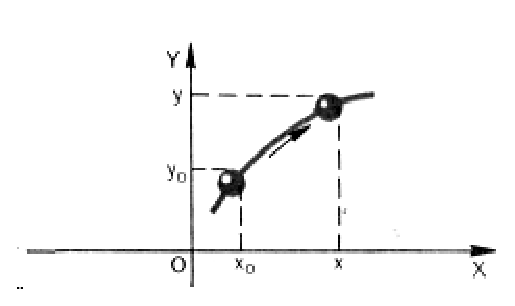
\includegraphics[width=0.2\textwidth]{img/img16.eps}
\caption{}
\label{kr_l}
\end{wrapfigure}

  Криволинейное движение более сложное, чем прямолинейное. И в природе и
в технике очень часто встречаются движения, траектории которых представляют
собой не прямые, а кривые линии. Это криволинейные движения. По криволинейным
траекториям движутся в космическом пространстве планеты и искусственные
спутники Земли, а на Земле - всевозможные средства транспорта, части машин и
механизмов, воды рек, воздух атмосферы и т. д.

  Криволинейное движение сложнее прямолинейного. При таком движении уже
нельзя сказать, что изменяется только одна координата. Если, например, движение
происходит на плоскости, то, как это видно из рисунка \ref{img_18}, изменяются две
координаты: $х$ и $у$. Непрерывно изменяется направление движения, т. е.
направление вектора скорости, а значит, и направление вектора ускорения. Могут
изменяться и модули скорости и ускорения. Все это и делает криволинейное
движение много сложнее прямолинейного.

\begin{figure}[h!]
\begin{center}
  % Requires \usepackage{graphicx}
  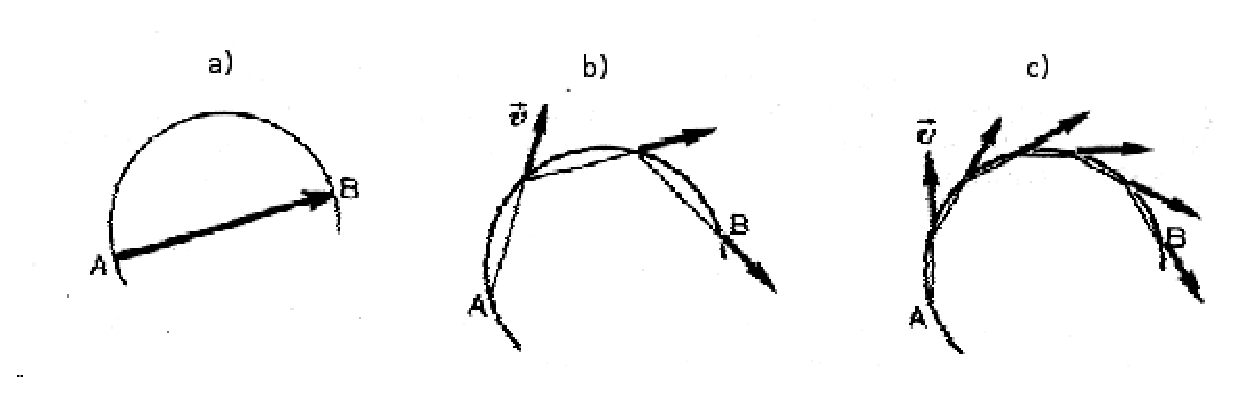
\includegraphics[width=0.7\textwidth]{img/img18.eps}\\
\end{center}
  \caption{}\label{img_18}
\end{figure}

\section{Перемещение и скорость при криволинейном движении}

  При прямолинейном движении направление вектора скорости всегда
совпадает с направлением перемещения. Что можно сказать о направлении
перемещения и скорости при криволинейном движении? Перемещение - по хордам.

\begin{wrapfigure}{l}{0.2\textwidth}
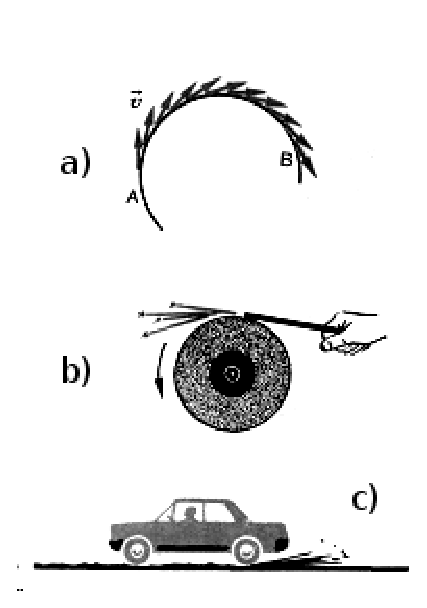
\includegraphics[width=0.2\textwidth]{img/img19.eps}
\caption{}
\label{ps_kl}
\end{wrapfigure}
  На рисунке $\ref{kr_l},\ a$ представлена некоторая криволинейная траектория.
Допустим, что тело движется по ней из точки А в точку В. Пройденный телом при
этом путь - это длина дуги АВ, а перемещение - это вектор, направленный по
хорде АВ. Теперь мы не можем сказать, что скорость всегда направлена вдоль
вектора перемещения. Но проведем между точками А и В ряд хорд и представим
себе, что тело движется именно по этим хордам. На каждой из них тело движется
прямолинейно, и вектор скорости направлен вдоль хорды, т. е. вдоль вектора
перемещения (рис. \ref{kr_l}, b). Мгновенная скорость - по касательной. Сделаем наши
 прямолинейные участки более короткими (рис. \ref{kr_l}, c). По-прежнему на каждом из
них вектор скорости направлен вдоль хорды. Но видно, что эта ломаная линия уже
больше походит на плавную кривую.

  Продолжая уменьшать длину прямолинейных участков (и, конечно,
увеличивая их число), мы как бы стягиваем их в точки, и ломаная линия
превращается в плавную кривую. Скорость же в каждой точке оказывается
направленной по касательной к кривой в этой точке (рис. \ref{ps_kl}, a).

  В том, что скорость при криволинейном движении действительно направлена
по касательной, убеждает нас, например, наблюдение за работой на точиле (рис. \ref{ps_kl}, b)
. Если прижать к вращающемуся точильному камню конец стального прутка, то
раскаленные частицы, отрывающиеся от камня, будут видны в виде искр. Эти
частицы летят с той скоростью, которой они обладали в момент отрыва от камня.
Хорошо видно, что направление движения искр совпадает с касательной к
окружности в той точке, где пруток касается камня. По касательной движутся и
брызги от колес буксующего автомобиля (рис. \ref{ps_kl}, c). Таким образом, мгновенная
скорость тела в разных точках криволинейной траектории имеет различные
направления. Но даже если по модулю скорость
тела не изменяется, ее все же нельзя считать постоянной. Ведь скорость -
величина векторная. А для векторных величин модуль и направление одинаково
важны. Поэтому криволинейное движение - это всегда движение с ускорением, даже
если по модулю скорость постоянна. Мы ограничимся рассмотрением именно такого
криволинейного движения - криволинейного движения с постоянной по модулю
скоростью. Его называют равномерным криволинейным движением. Ускорение при
таком движении связано с изменением направления скорости. Как направлено и чему
равно это ускорение?

  Криволинейное движение - движение по дугам окружностей. Изменение
скорости по направлению при криволинейном движении должно, конечно, зависеть от
формы траектории. А различных форм кривых линий есть бесчисленное множество. Но
оказывается, не нужно рассматривать движения по каждой отдельной кривой.

\begin{wrapfigure}{l}{0.3\textwidth}
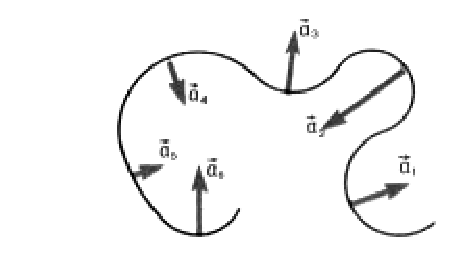
\includegraphics[width=0.3\textwidth]{img/img_20.eps}
\caption{}
\label{r62}
\end{wrapfigure}

  На рисунке \ref{r62} показана некоторая сложная криволинейная траектория. Из
рисунка видно, что отдельные части криволинейной траектории представляют собой
приблизительно дуги окружностей. Движение по любой криволинейной траектории
можно приближенно представить как движение по дугам некоторых окружностей.
Поэтому задача нахождения ускорения при равномерном криволинейном движении
сводится к отысканию ускорения при равномерном движении тела по окружности.

\section{Ускорение при  равномерном движении   по окружности}

  Равномерное движение по окружности - это движение с ускорением, хотя по
модулю скорость не изменяется. Наша задача выяснить, как направлено и чему
равно это ускорение.

  Докажем, что вектор ускорения направлен к центру окружности. Ускорение,
как известно, определяется равенством
\[
\vec{a}=\frac{d\vec{v}}{dt}=\frac{\vec{v}-\vec{v}_0}{t}
\]

Обозначим для краткости разность двух значений скорости $\Delta v$.

  Ясно, что вектор $\vec{a}$ направлен так же, как вектор $\Delta\vec{a}$,
потому что $t$ - величина скалярная.

\begin{wrapfigure}{l}{0.3\textwidth}
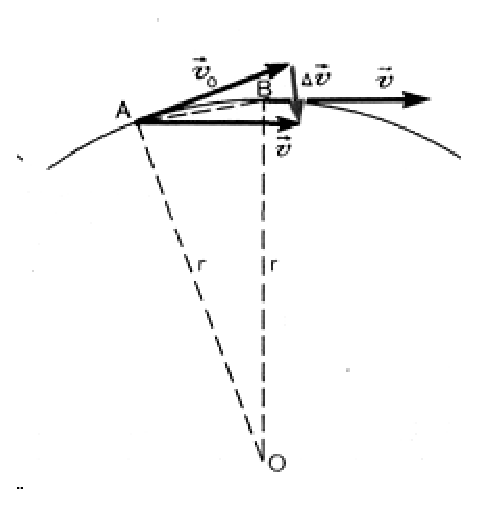
\includegraphics[width=0.3\textwidth]{img/img_21.eps}
\caption{}
\label{r60}
\end{wrapfigure}
  Допустим, что тело движется по окружности радиусом $r$ и в некоторый момент
времени, который мы примем за начальный $(t = 0)$, оно находится в точке $А$
(рис. \ref{r60}). Скорость $v_0$ в этой точке направлена по касательной. Рассмотрим
еще одну точку, очень близкую к точке $А$, - точку $В$, в которой тело,
двигаясь по окружности, окажется через очень малый промежуток времени $t$.
Будем считать, что точки $A$ и $В$ настолько близки друг к другу, что дуга
$АВ$ неотличима от хорды $АВ$, хотя на рисунке это и нельзя изобразить. Но
как бы точка $В$ ни была близка к точке $А$, скорость $v$ в точке $В$ все же
отличается от скорости $v_0$ направлением, хотя и не отличается от нее по
модулю $(v_0 = v)$. Теперь мы можем найти вектор $\Delta v$: перенесем вектор
$v$ параллельно самому себе так, чтобы он и вектор $v_0$ исходили из точки
$А$, и соединим концы обоих векторов отрезком прямой, направив его от $v_0$ к
$v$. Получившийся направленный отрезок и есть вектор $\Delta v$. Из рисунка
видно, что вектор $\Delta v$ направлен внутрь окружности. И если точки $А$ и
$В$ будут предельно близки друг к другу, то вектор $\Delta v$, перенесенный в
точку $А$, будет направлен к центру окружности. Туда же будет направлен и
вектор ускорения $\vec{a}$. Таким образом, при равномерном движении тела по
окружности его ускорение во всех точках окружности <<устремлено>> к ее центру.
Его так и называют центростремительным ускорением. Обозначим его $а$.

\begin{wrapfigure}{l}{0.3\textwidth}
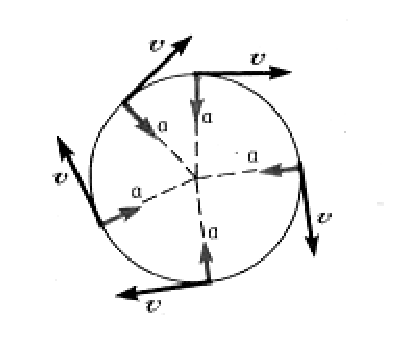
\includegraphics[width=0.3\textwidth]{img/img_22.eps}
\caption{}
\label{r63}
\end{wrapfigure}
  Ускорение тела, равномерно движущегося по окружности в любой ее точке,
центростремительное, т. е. направлено по радиусу окружности к ее центру. В
любой точке вектор ускорения перпендикулярен вектору скорости. Эта особенность
ускорения при равномерном движении по окружности показана на рисунке \ref{r61}.

  Чему равен модуль центростремительного ускорения? Числовое значение
(модуль) ускорения мы легко найдем из рисунка \ref{r60}. Треугольник, составленный из
 векторов $v_0$ и $v$, равнобедренный, так как $v_0=v$. Треугольник $ОАВ$ на
том же рисунке тоже равнобедренный, потому что стороны $ОА$ и $ОВ$ - радиусы
окружности. Углы при вершинах обоих треугольников равны, так как они
образованы взаимно перпендикулярными сторонами. Поэтому треугольники подобны,
как равнобедренные с равными углами при вершинах. Из подобия треугольников
следует пропорциональность сходственных сторон: $\frac{\Delta
v}{AB}=\frac{v}{r}$. Но, как указывалось раньше, если точки $А$ и $В$ очень
близки друг к другу, то хорда $АВ$ неотличима от дуги $АВ$. Длина же дуги $АВ$ -
 это путь, пройденный телом с постоянной по модулю скоростью $v$. Он равен
$vt$. Поэтому можно написать: $\frac{\Delta v}{vt}=\frac{v}{t}$ или
$\frac{\Delta v}{t}=\frac{v^2}{r}$, т.е. $a=\frac{v^2}{r}$. Таким образом, при
равномерном движении по окружности во всех ее точках ускорение по модулю одно
и то же - $а$. Но направлено оно всегда по радиусу к центру (см. рис. 61), так
что направление ускорения от точки к точке изменяется. Равномерное движение
по окружности нельзя назвать равноускоренным.

  Напомним, что равномерное движение по окружности нас интересовало
потому, что всякое движение по криволинейной траектории можно представить как
движение по дугам окружностей различных радиусов.

  Теперь мы можем сказать, что в любой точке криволинейной траектории
тело движется с ускорением, направленным к центру той окружности, частью
которой является участок траектории, содержащий эту точку. Модуль же ускорения
зависит от скорости тела и от радиуса соответствующей окружности. На рисунке \ref{r62}
показана некоторая сложная траектория, по которой движется тело, и
центростремительные ускорения тела в различных ее точках.

  В общем случае, когда скорость меняется и по модулю и по направлению вектор
ускорения направлен под некоторым углом к вектору скорости. Обычно его
представляют как сумму двух составляющих $\vec{a}=\vec{a}_r+\vec{a}_n$,
тангенсальное ускорение $\vec{a}_r$ и направлено оно по касательной к
траектории и характеризует изменение модуля скорости $\vec{a}_r=\frac{v-
v_0}{t}$, нормальное ускорение (центростремительное) $\vec{a}_n=\frac{v^2}{r}$
 направлено по радиусу кривизны траектории. $a=\sqrt{a^2_r+a^2_n}$. Угол между
скоростью и ускорением равен: $a=\arctg\ \frac{a_n}{a_r}$.

\begin{center}
   Вопросы
\end{center}
\begin{enumerate}
\item Что такое путь при движении по окружности?
\item Что является перемещением при движении по окружности?
\item Как направлена скорость при криволинейном движении?
\item Как направлено центростремительное ускорение?
\item Чему равен модуль центростремительного ускорения?
\item Что характеризует тенгенсальное ускорение?
\item Чему равно полное ускорение тела, движущегося по окружности?
\end{enumerate}

\section{Период и частота обращения}

\begin{wrapfigure}{l}{0.3\textwidth}
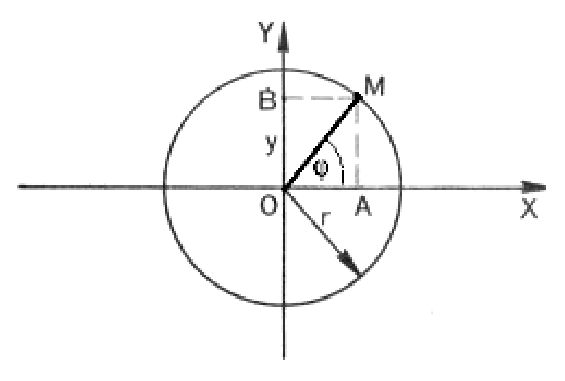
\includegraphics[width=0.3\textwidth]{img/img_23.eps}
\caption{}
\label{r63}
\end{wrapfigure}
  Движение тела по окружности часто характеризуют не скоростью $v$ движения
тела, а угловой скоростью $\omega$ (омега) и промежутком времени, за который
тело совершает один полный оборот - период обращения
$\omega=\frac{d\phi}{dt}$ и т.д. Так, например, в сообщениях о запуске
очередного искусственного спутника Земли указывается именно период его
обращения, а не скорость его движения по орбите. Но если известен период
обращения $Т$, то легко найти и скорость $v$. Действительно, за время, равное
периоду $Т$, тело проходит путь, равный длине окружности $L=2\pi r$, где $r$
- радиус окружности, по которой движется тело $T=\frac{2\pi r}{v}$. Отсюда
линейная скорость равна $v=\frac{2\pi r}{T}$.

  Движение тела (точки) по окружности, можно характеризовать еще одной
величиной - числом оборотов по окружности в единицу времени. Ее называют
частотой обращения и обозначают буквой $n$. $n=\frac{1}{T}$.
Центростремительное ускорение можно теперь найти по формуле $a=4\pi^2 n^2 r$.
Теперь можно сказать, что чем дальше от центра окружности, тем больше
ускорение точек.

  Период и угловая скорость связаны соотношением $N=\frac{2\pi}{\omega}$. Угловая и линейная
скорость связаны соотношением $v=\omega r$.

\begin{center}
   Вопросы
\end{center}
\begin{enumerate}
\item Что называется угловой скоростью?
\item Что такое период?
\item Как определить линейную скорость?
\item Как определить период вращения?
\item Что такое частота вращения?
\item Как выглядит уравнение движения для тела вращающегося вокруг неподвижной оси?
\end{enumerate}

\begin{center}
   Домашнее задание
\end{center}
\begin{enumerate}
\item Частота обращения ветроколеса ветродвигателя 30 об/мин, якоря электродвигателя 1500 об/мин, барабана сепаратора 8400 об/мин, шпинделя шлифовального станка 96000 об/мин. Вычислить их периоды.
\item Найти частоту обращения Луны вокруг Земли.
\item Скорость точек рабочей поверхности наждачного  круга диаметром 300 мм не должна превышать 35 м/с. Допустима ли посадка круга на вал электродвигателя, совершающего 1400 об/мин; 2800 об/мин?
\item Частота обращения воздушного винта самолета 1500 об/мин. Сколько оборотов делает винт на пути 90 км при скорости полета 180 км/ч?
\item Период обращения платформы карусельного станка 4 с. Найти скорость крайних точек платформы, удаленных от оси вращения на 2 м.
\item Диаметр передних колес трактора в 2 раза меньше, чем задних. Сравнить частоты обращения колес при  движении трактора.
\item Радиус рукоятки колодезного ворота в 3 раза больше радиуса вала, на который наматывается трос. Какова  линейная скорость конца рукоятки при поднятии ведра с глубины 10 м за 20 с?
\item С какой скоростью и в каком направлении должен  лететь самолет по шестидесятой параллели, чтобы прибыть в пункт назначения раньше (по местному времени), чем он  вылетел из пункта отправления? Возможно ли это для  современных пассажирских самолетов?
\item При увеличении в 4 раза радиуса круговой орбиты искусственного спутника Земли период его обращения увеличивается в 8 раз. Во сколько раз изменяется скорость движения спутни ка по орбите?
\item Минутная стрелка часов в 3 раза длиннее секундной. Найти отношение скоростей концов стрелок.
\item Циркулярная пила имеет диаметр 600 мм. На ось пилы насажен шкив диаметром 300 мм, который  приводится во вращение посредством ременной передачи от шкива диаметром 120 мм, насаженного на вал электродвигателя.  Какова скорость зубьев пилы, если вал двигателя совершает 1200 об/мин?
\item Диаметр колеса велосипеда <<Пенза>> $d$ = 70 см,  ведущая звездочка имеет $z_1$ = 48 зубцов, а ведомая $z_2$ = 18 зубцов. С какой скоростью движется велосипедист на этом велосипеде при частоте вращения педалей $n$ = 1 об/с? С какой скоростью движется велосипедист на складном велосипеде <<Кама>> при той же частоте вращения педалей, если у этого велосипеда  соответственно $d$ = 50 см, $z_1$ = 48 зубцов, $z_2$ = 15 зубцов?
\item Каково центростремительное ускорение поезда,  движущегося по закруглению радиусом 800 м со скоростью 20 м/с?
\item Скорость точек экватора Солнца при его вращении вокруг своей оси равна 2 км/с. Найти период обращения  Солнца вокруг своей оси и центростремительное ускорение точек экватора.
\item Период обращения молотильного барабана комбайна <<Нива>> диаметром 600 мм равен 0,046 с. Найти скорость точек, лежащих на ободе барабана, и их центростремительное ускорение.
\item С какой скоростью автомобиль должен проходить  середину выпуклого моста радиусом 40 м, чтобы  центростремительное ускорение было равно ускорению свободного  падения?
\item Рабочее колесо турбины Красноярской ГЭС имеет диаметр 7,5 м и вращается с частотой 93,8 об/мин. Каково центростремительное ускорение концов лопаток турбины?
\item Найти центростремительное ускорение точек колеса автомобиля, соприкасающихся с дорогой, если автомобиль движется со скоростью 72 км/ч и при этом частота обращения колеса 8 $с^{-1}$.
\item Радиус рабочего колеса гидротурбины в 8 раз  больше, а частота обращения в 40 раз меньше, чем у паровой  турбины. Сравнить скорости и центростремительные ускорения точек обода колес турбин.
\item Детский заводной автомобиль, двигаясь равномерно, прошел расстояние $s$ за время $t$. Найти частоту обращения и центростремительное ускорение точек на ободе колеса, если диаметр колеса равен $d$.
\end{enumerate}

\section{Как изменяются координаты тела со временем при равномерном движении по окружности}

  Допустим, что некоторое тело равномерно движется по окружности радиусом
$r$. Систему координат удобно (хотя и необязательно) выбрать так, чтобы начало
координат совпадало с центром окружности, а оси X и Y были направлены вдоль
двух взаимно перпендикулярных диаметров (рис. \ref{r63}).

  Пусть при своем движении тело в какой-то момент времени находится в
точке М на окружности. Координата х в этот момент равна отрезку ОА на
горизонтальном диаметре, а координата у - отрезку ОВ на вертикальном.

\begin{gather*}
x=r\cdot\cos\ \phi,\ y=r\cdot\sin\ \phi\ \\
или\ с\ учётом\ угловой\ скорости\\
x=r\cdot\cos\ \omega\ t,\ y=r\cdot\sin\ \omega\ t \\
\end{gather*}

  Координаты повторяются через промежуток времени, который называется период
обращения $Т$, тело снова окажется в точке $М$ и его координаты $х$ и $у$ будут
 снова равны $ОА$ и $ОВ$ соответственно. Такими же они будут и через два
периода, и через три периода и т. д. Это и есть главная особенность движения
по окружности - координаты тела через каждый период обращения повторяются.

  Равномерное движение по окружности- это периодическое движение. Из
того, что мы уже знаем о скорости и ускорении тела, равномерно движущегося по
окружности, ясно, что и эти величины тоже изменяются периодически: через каждый
период повторяются и численные значения, и направления скорости и ускорения.

  Такого рода периодические изменения величин называют колебаниями.
Построение графиков $x=r\cdot\cos\ \phi$ с помощью окружности.

\section{Движение на вращающемся теле}

  Все мы живем на поверхности земного шара, который вращается (вместе с
нами!) вокруг своей оси. Мы, однако, этого вращения не замечаем, если не
считать смены дня и ночи, вызванной этим вращением. Но не замечаем мы этого
вращения потому, что вращается Земля очень медленно. Один оборот Земля делает
за сутки.

\begin{wrapfigure}{l}{0.2\textwidth}
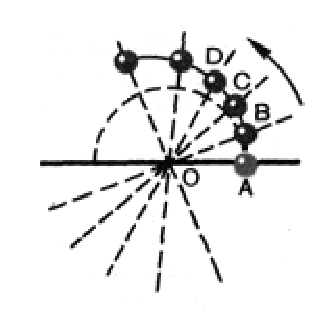
\includegraphics[width=0.2\textwidth]{img/img_24.eps}
\caption{}
\label{r65}
\end{wrapfigure}
  Но если какое-нибудь тело вращается с достаточно большой частотой, то
всякое тело, на нем находящееся, совершает очень любопытное движение. Его легко
наблюдать, если проделать простой опыт: небольшое проволочное кольцо надеть на
стержень (спицу, карандаш и т.д.) и быстро повернуть стержень. Кольцо со
стержня соскользнет. Почему оно соскальзывает?

  Рассмотрим этот опыт более подробно.

  Представим себе стержень, на который надет просверленный шарик. Пусть
стержень вращается вокруг оси, проходящей через его середину (рис. \ref{r65}). Чтобы
выяснить, как должен себя вести шарик, будем вращение рассматривать как
множество последовательных малых поворотов вокруг оси.

  Как ведет себя шарик при таких поворотах? Пусть в некоторый момент
времени шарик находится в точке $А$ на расстоянии $ОА$ от оси вращения. Если бы
шарик был в этом положении закреплен на стержне, то при вращении он двигался бы
по окружности радиусом $ОА$, показанной штриховой линией на рисунке. Но шарик не
закреплен. Поэтому он станет двигаться вдоль вектора скорости, который, как мы
знаем, направлен по касательной к окружности, т. е. перпендикулярно $ОА$. Когда
стержень совершит малый поворот, шарик окажется в точке $В$. Ясно, что $ОВ$
больше, чем $ОА$, потому что треугольник ОАВ прямоугольный и в нем сторона $ОВ$-
гипотенуза, а $ОА$ - катет.

  При следующем малом повороте шарик опять продвинется перпендикулярно
новому положению стержня. Мы видим, что при вращении стержня шарик все время
удаляется от оси, скользя вдоль стержня.

\begin{center}
   Вопросы
\end{center}
\begin{enumerate}
\item Как   направлена   мгновенная   скорость при криволинейном движении?
\item Чем различаются  изменения скорости при прямолинейном и криволинейном движениях?
\item Могут ли  при  криволинейном движении   совпадать   направления   векторов   скорости и ускорения?
\item Может   ли   тело   двигаться   по   криволинейной траектории без ускорения?
\item Какая    связь    между    криволинейным движением    и    движением    по   окружности?
\item Как направлено ускорение тела,  движущегося   по   окружности   с   постоянной   по модулю скоростью?
\item Можно ли считать центростремительное  ускорение  постоянным,  а  равномерное движение     по     окружности     равноускоренным?
\item Если   при   движении   тела   по   окружности   модуль   скорости   изменяется,   будет ли    ускорение   тела    направлено    к    центру окружности?
\item Катер со спортсменом на водных лыжах движется по окружности. Спортсмен может следовать за катером по той же окружности, но может двигаться и вне и внутри окружности. Каково соотношение скоростей спортсмена и катера в этих трех случаях?
\item Что такое период обращения?
\item Что такое частота обращения?
\item Как  связаны  между  собой   период  и частота обращения?
\item Как выражается центростремительное ускорение через период обращения?
\item Как выражается центростремительное ускорение через частоту обращения?
\end{enumerate}

\begin{center}
   Задачи
\end{center}
\begin{enumerate}
\item Точильный круг радиусом 10 см делает  один  оборот  за 0,2 с. Найдите  скорость точек,   наиболее   удаленных   от   оси   вращения.
\item Автомобиль движется по закруглению дороги радиусом 100 м. Чему равно центростремительное ускорение  автомобиля,  если он движется со скоростью 54 км/ч?
\item Период   обращения    первого    космического корабля - спутника Земли <<Восток>> равнялся 90 мин. Средняя высота спутник; над Землей была равна 320 км. Радиус Земли 6400 км. Вычислите скорость корабля.
\item Какова скорость  движения автомобиля, если его колеса радиусом 30 см делают 600 оборотов в минуту?
\item Луна движется  вокруг Земли  на расстоянии  380 000  км  от  нее,   совершая  один оборот за 27,3 сут. Вычислите центростремительное ускорение Луны.
\item Пропеллер самолета радиусом 1,8 м вращается при посадке с частотой 2200 $мин^{-1}$, посадочная скорость самолета относительно Земли равна 120 км/ч. Определите скорость точек на конце пропеллера. Какова траектория движения этой точки?
\end{enumerate}

\begin{center}
   Домашнее задание
\end{center}
\begin{enumerate}
\item Автомобиль движется по закруглению дороги радиусом 220 м со скоростью 72 км/ч. Чему равно центростремительное ускорение автомобиля?
\item Вал диаметром 30 см при вращении делает один оборот за 0,6 с. Определите линейную скорость точек на поверхности вала
\item Диск диаметром 60 см равномерно перекатывают на расстояние 8 м за 4 с. Какова угловая скорость вращения диска?
\item Радиус одного колеса 30 см, другого - 60 см, а линейные скорости точек на ободе колес соответственно равны 2,5 и 7,5м/с. Во сколько раз центростремительное ускорение точек на ободе одного колеса больше, чем на ободе другого?
\item Пропеллер самолета радиусом 2 м вращается при посадке с частотой 1500 мин-1, посадочная скорость самолета относительно Земли равна 144 км/ч. Определите скорость точек на конце пропеллера. Какова траектория движения этой точки?
\item Найти радиус вращающегося колеса, если известно, что линейная скорость точки лежащей на ободе в 4 раза больше линейной скорости точки, лежащей на 6 см ближе к оси колеса.
\item Первая в мире орбитальная космическая станция двигалась со скоростью 7,8 км/с и имела период обращения 88,85 мин. Считая ее орбиту круговой, найти высоту станции над поверхностью Земли. Радиус Земли принять равным 6400 км.
\item Мальчик вращает камень, привязанный к веревке длиной 0,7 м в вертикальной плоскости так, что частота равна 5 об/с. На какую высоту взлетел камень, если веревка оборвалась к тот момент, когда скорость была направлена вертикально вверх?
\end{enumerate}

\section{Решение задач}

\subsection{I ВАРИАНТ}
\begin{enumerate}
\item Движение точки на плоскости описывается уравнениями х = 6 + 3t, у = 4t. Определить траекторию движения точки и построить ее на плоскости ХОУ.
\item Из городов А и В, расстояние между которыми 120 км, одновременно выехали навстречу две автомашины, скорости которых постоянны и равны 20 км/ч и 60 км/ч. Найти, через какое время и на каком расстоянии от города С, находящегося на полпути между А и В, встретятся автомобили.
\\ Ответ: 1,5ч. 30км
\item Моторная лодка проходит по реке от пункта А до пункта В расстояние за 4 часа, а обратно - за 5 часов. Определите скорость течения реки, если расстояние между пунктами 80 км.
\\ Ответ: 2,5 км/ч
\item Тело, имея начальную скорость 5 м/с, прошло за пятую секунду путь, равный 4,5 м. Определить ускорение и путь, пройденный телом за 10 с.
\\ Ответ: $-0,11м/с^2$.  44,5м

\item Мальчик вращает камень, привязанный к веревке длиной 0,5 м в вертикальной плоскости так, что частота равна 3 об/с. На какую высоту взлетел камень, если веревка оборвалась к тот момент, когда скорость была направлена вертикально вверх?
\end{enumerate}

\subsection{II ВАРИАНТ}
\begin{enumerate}
\item Точка М совершает движение на плоскости ХОУ. Координаты точки в зависимости от времени изменяются так: х = -4t, у = 6 + 2t. Записать уравнение траектории у = у(х) точки
\item Из двух пунктов, расстояние между которыми 100 м, одновременно навстречу друг другу начали двигаться два тела. Скорость одного из них 20 м/с. Какова скорость второго тела, если они встретились через 4 с? Начало координат поместите в пункте нахождения тела, скорость которого известна.
\\ Ответ: 5м/с.

\item Между двумя пунктами, расположенными на реке на расстоянии 100 км один от другого, курсирует катер, который, идя по течению, проходит это расстояние за время 4 часа, а против течения - за время 10 ч. Определить скорость течения реки и скорость катера относительно воды.
\\ Ответ: 7,5км/ч
\item Пуля, летящая со скоростью 400 м/с, ударяет в земляной вал и проникает в него на глубину 36 см. Сколько времени двигалась она внутри вала? С каким ускорением? Какова была ее скорость на глубине 18 см?
\\ Ответ: $1,8\cdot 10^{-4}с$.  $2,21\cdot 105м/с^2$.  282м/с.
\item Пропеллер самолета радиусом 1,5 м вращается при посадке с частотой 2000 мин-1, посадочная скорость самолета относительно Земли равна 162 км/ч. Определите скорость точек на конце пропеллера. Какова траектория движения этой точки?
\end{enumerate}

\section{Сила}

  Физические объекты проявляют себя в движении и взаимодействии. Мерой
взаимодействия тел или частиц, из которых состоят тела, является сила.
Результатом взаимодействия тел является либо деформация (изменение размеров),
либо ускорение (изменение скорости). Каждое из этих проявлений силы может быть
использовано для её измерения. Измерить величину деформации часто проще, чем
измерить ускорение. Поэтому основной деталью прибора для измерения сил -
динамометра - является пружина, степень деформации которой зависит от величины
измеряемой силы.

  Рассмотрим опыт по взаимодействию магнита с куском железа (см.
рисунок \ref{rm}). Динамометры, прикреплённые к обоим телам, регистрируют одинаковые по
величине деформации. Это значит, что действие одного тела на другое равно
действию другого тела на первое.

\begin{figure}
\begin{center}
  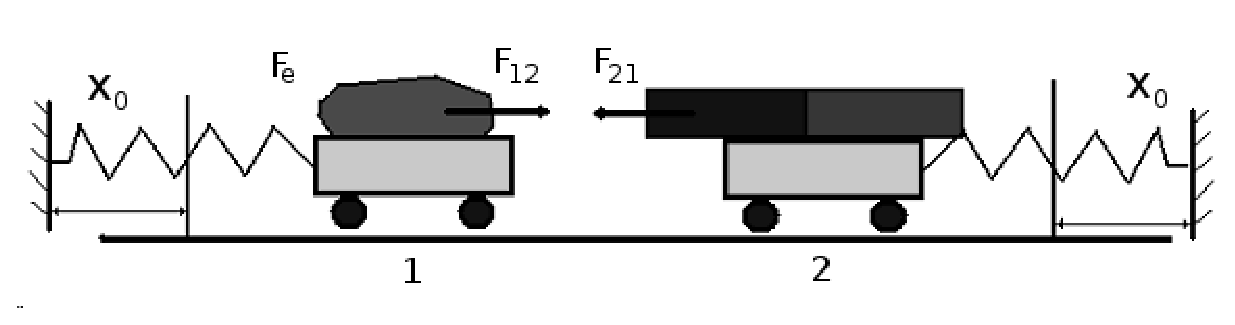
\includegraphics[width=0.7\textwidth]{img/ris_25.eps}\\
\end{center}
\caption{}\label{rm}
\end{figure}

\textbf{То есть сила действия одного тела на другое
равна силе действия второго на первое}.
Это III закон Ньютона $\vec{F}_{12}=-\vec{F}_{21}$.

  Опираясь на этот закон можно определять силу, действующую на одно тело с
помощью измерения силы действующей на другое тело.

  Из практики известно, что чем большую деформацию мы желаем создать, тем
большее усилие нужно приложить к деформируемому телу. \textbf{При малых деформациях
величина деформации пропорциональна приложенной силе (закон Гука)}.
\[
F=k(l-l_0)=k\Delta l
\]
 где $F$ - абсолютная величина силы, $l_0$ - первоначальная длина тела, $l$ -
длина деформированного тела и $К$ - коэффициент упругости.

  Из закона Гука следует, что шкала динамометра должна быть равномерной.

  Всякая сила имеет направление, причём результат действия силы зависит не
только от её величины, но и от направления силы. Например, ударяя по мячу в
разные стороны, футболист сообщает мячу ускорение разного направления.

  В реальности на тело могут действовать множество сил. Сила, действие
которой эквивалентно действию всех сил, действующих на тело, называется
равнодействующей всех сил. Если линии действия сил сходятся в одной точке, то
такая совокупность сил называется системой сходящихся сил (пучком сил).
Равнодействующая системы сходящихся сил, действующих на тело равна
геометрической сумме сил.
\[
\vec{F}=\sum\limits_{i=1}^{k}\vec{F}_i
\]

  В самом общем случае действие произвольной системы сил на абсолютно
твёрдое тело эквивалентно действию на тело главного момента системы сил
относительно центра приведения и главного вектора системы сил, равного
геометрической сумме сил системы. Точка О приложения главного вектора системы
сил (центр приведения) выбирается произвольно и влияет только на величину
главного момента системы сил (сумма моментов всех сил относительно этой точки,
т.е. центра приведения).

  Силы могут быть сосредоточенными, действующими в одной точке и
распределёнными, действующими на определённую часть поверхности. Автомобиль,
стоящий на мосту - сосредоточенная сила, действующая на мост. Поезд, проходящий
по мосту - распределённая сила (нагрузка).

  Вычислить силу можно по ускорению, которое тело приобретает под действием
этой силы. Из курса физики 7 класса известно, что сила тяжести равна $F=mg$,
где $m$ - масса тела, $g$ - ускорение свободного падения. Масса входящая в
эту формулу называется гравитационной, т.к. является мерой взаимодействия
тела с Землёй.

  Рассмотрим движение тела по окружности. Тело движется равномерно по
окружности радиуса $R$ с угловой скоростью $\omega$ под действием силы
упругости $F=kx$ определяемой с помощью динамометра. Под действием этой силы
тело приобретает центростремительное ускорение $а=\omega^2R$. Проделав опыты с
 телами различной массы, убедимся, что сила пропорциональна массе и
центростремительному ускорению. Масса, входящая в данную формулу называется
инертной т.к. влияет на изменение скорости движения. Будем считать, что
инертная и гравитационная массы равны. Причём произведение массы на
центростремительное ускорение будет равно силе, которую показывает
динамометр. Эта сила называется центростремительной: $\vec{F}=m\vec{a}$. Эта
формула выражает II закон Ньютона (основной закон динамики поступательного
движения).

\begin{wrapfigure}{l}{0.2\textwidth}
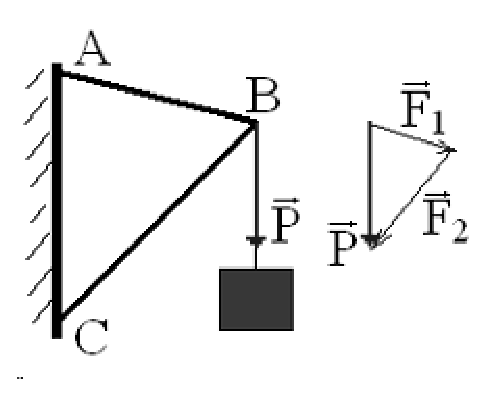
\includegraphics[width=0.2\textwidth]{img/ris_26.eps}
\caption{}
\label{r26}
\end{wrapfigure}
  Если действующие на материальную точку можно заменить одной силой -
равнодействующей системы сил, то возможно и обратное действие - силу,
действующую на материальную точку можно разложить на несколько сил, сумма
которых равна данной силе. Например: на кронштейне подвешено тело (рис. \ref{r26}). Его вес
действует на точку подвеса. Чтобы найти силы, возникающие в стержнях необходимо
разложить силу веса по направлениям, параллельным стержням. Тогда $\vec{F_1}$, является
растягивающей силой, а $\vec{F_2}$ сжимающей силой. Из подобия треугольников следует:
\[
\frac{F_1}{AB}=\frac{F_2}{BC}=\frac{P}{AC}
\]

\begin{center}
   Вопросы
\end{center}
\begin{enumerate}
\item Что такое сила?
\item Как можно измерить силу?
\item Сформулируйте III закон Ньютона
\item Сформулируйте закон Гука
\item Что называется равнодействующей сил
\item Чему равна равнодействующая сходящихся сил
\item Какие бывают силы?
\item Сформулируйте II закон Ньютона
\end{enumerate}

\begin{center}
   Задачи
\end{center}
\begin{enumerate}
\item Под действием силы пружина, жёсткостью 1кН/м растянулась на 1см. Определить модуль силы.
\item Под действием какой силы пружина, имеющая жесткость 10000 Н/м, сжалась на 4 см?
\item Чему равна жесткость латунного стержня, если под действием груза 1000 Н он удлинился на 1 мм?
\item Определите удлинение пружины, если на нее действует сила 10 Н, а жесткость пружины 500 Н/м.
\item Паровоз толкнул вагон массой 30 т, стоящий на горизонтальном пути. Вагон начал двигаться со скоростью 0,5 м/с. Определите силу удара, если его длительность 1 с.
\item За какое время тело массой 100 г изменит свою скорость от 5 м/с до 15 м/с под действием силы 0,5 Н?
\item Снаряд массой 15 кг при выстреле приобретает скорость 600 м/с. Найдите среднюю силу, с которой пороховые газы давят на снаряд, если длина ствола орудия 1,8 м. Движение снаряда в стволе считайте равноускоренным.
\item На кронштейне подвешено тело весом 10Н. АВ=30см, ВС= 60см АС=70см. Определить реакции связи (силы упругости в стержнях). Начертите чертёж.
\item На кронштейне подвешено тело весом 10Н. АВ=30см, ВС= 50см АС=40см. Определить реакции связи (силы упругости в стержнях). Начертите чертёж.
\end{enumerate}

\section{Импульс. Закон сохранения импульса. II закон ньютона.
Взаимодействие двух или нескольких тел.}

Вернёмся к 3 закону Ньютона.
\[
\vec{F}_12=-\vec{F}_21\to m_1\vec{a}_1=m_2\vec{a}_2\to
m_1\Delta\vec{v}_1=-m_2\Delta\vec{v}_2\to
m_1\vec{v}_1+m_2\vec{v}_2=m_1\vec{v}_1^1+m_2\vec{v}_2^1
\]

  \textbf{В замкнутой системе сумма импульсов тел до взаимодействия равна сумме
импульсов тел после взаимодействия.}

  Это закон сохранения импульсов тел. Произведение массы на скорость тела
называется количеством движения или импульсом тела и измеряется в килограмм-
метрах в секунду (кг$\cdot$ м/с).

\textbf{  В замкнутой системе сумма импульсов тел - величина
постоянная. }
\[
\frac{m_1}{m_2}=-\frac{\Delta v_2}{\Delta v_1}\to
m_1=-m_2\frac{\Delta v_2}{\Delta v_1}
\]

 Если за $m_2$ принять эталонную массу, то определённая таким способом масса
называется инертной и характеризует способность тела сохранять свою скорость.

\textbf{Пример 1}:

 Вагон массой 20 т, движущийся со скоростью 0,3 м /с, нагоняет вагон массой 30
т, движущийся со скорость 0,2 м /с, после упругого столкновения второй вагон
стал двигаться со скоростью 0,25 м /с. Определите скорость первого вагона.
%\intextsep=-3mm
\begin{wrapfigure}{l}{0.25\textwidth}
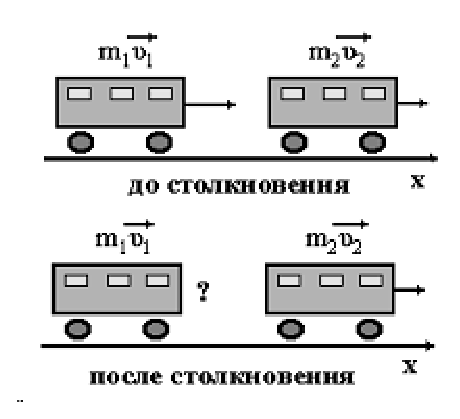
\includegraphics[width=0.25\textwidth]{img/img_27.eps}
\label{r27}
\end{wrapfigure}

\hspace{1cm}\textbf{Дано:}\hspace{.3cm}
\parbox[t]{4cm}{
$m_1=$20 т\\
$v_1=$0,3 м/с\\
$m_2=$30 т\\
$v_2=$0,2 м/с\\
$v_2'=$0,25 м/с\\
\rule{4cm}{.4pt}\\
$v_1'=?$\\
}


  \textbf{Решение:}

Записываем закон сохранения импульса в векторной форме:
\[
m_1\vec{v}_1+m_2\vec{v}_2=m_1\vec{v}_1^1+m_2\vec{v}_2^1
\]

спроектируем вектора на ось $ОХ$
\[
m_1 v_{1x}+m_2 v_{2x}=m_1 v_{1x}'+m_2 {v}_{2x}'
\]
\[
v_1^1=\frac{m_1 v_{1x}+m_2 v_{2x}-m_2 v_{2x}^1}{m_1}=
\frac{20\cdot10^3\cdot0,3+30\cdot10^3\cdot0,2-30\cdot10^3\cdot0,25}{20\cdot10^3}=
0,225\ м/с
\]

\textbf{Ответ:} после столкновения первый вагон будет двигаться со скоростью 0,225м/с.
Знак <<+>>  говорит о том, что скорость ${v_1}'$ направлена вдоль оси $ОХ$.

 \textbf{Пример 2}: С судна массой 600т произведен выстрел из пушки под углом
60\textdegree к горизонту. Какова стала скорость судна, если оно не двигалось?
Скорость снаряда 1000 м /с, а его масса 50 кг.


\begin{figure}
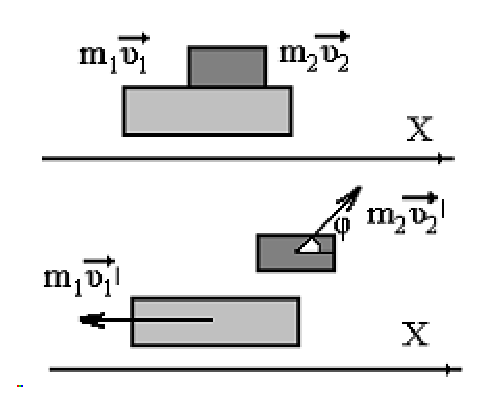
\includegraphics[width=0.75\textwidth]{img/img_28.eps}
\end{figure}

\vspace*{2cm}
\hspace{1cm}\textbf{Дано:}\hspace{.3cm}
\parbox[t]{4cm}{
$m_1=$600 т\\
$v_1=$0 м/с\\
$m_2=$50 кг\\
$v_2'=$1000 м/с\\
\rule{4cm}{.4pt}\\
$v_1'=?$\\
}



\vspace{10pt}
  \textbf{Решение:}

  Запишем закон сохранения импульса:
\[
m_1\vec{v}_1+m_2\vec{v}_2=m_1\vec{v}_1^1+m_2\vec{v}_2^1
\]


  Рассмотрим движение судна вдоль оси $Х$. Систему можно считать замкнутой
только в начальный момент времени.

  Спроектируем импульсы на ось $ОХ$.

\[
0=m_1 v_1'+m_2 v_2' \cos\ \phi
\]
\[
v_1'=-\frac{m_2 v_2\cdot \cos\ \phi}{m_1}=-\frac{50\cdot1000\cdot0.5}{600000}=
-0,042\ м/c
\]


Знак <<->> говорит о том, что $v_1'$ направлена против  оси $ОХ$.

\textbf{Ответ:} после выстрела корабль приобретёт скорость $0,042\ м/с$.


  \textbf{Пример 3}: Вагон массой 10 т двигается со скоростью 0,1 м/с.
Навстречу ему двигается вагон массой 30т со скоростью 0,5 м/с. Определить
скорость вагонов после срабатывания автосцепки.


\begin{wrapfigure}{l}{0.25\textwidth}
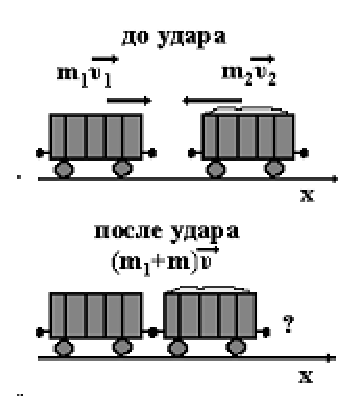
\includegraphics[width=0.25\textwidth]{img/img_29.eps}
\label{r29}
\end{wrapfigure}
\hspace{1cm}\textbf{Дано:}\hspace{.3cm}
\parbox[t]{4cm}{
$m_1=$10 т\\
$v_1=$0,1 м/с\\
$m_2=$30 т\\
$v_2=$0,5 м/с\\
\rule{4cm}{.4pt}\\
$v=?$\\
}

  \textbf{Решение:}

  Записываем закон сохранения импульса:
\[
m_1\vec{v}_1+m_2\vec{v}_2=m_1\vec{v}_1^1+m_2\vec{v}_2^1
\]

  Спроектируем импульсы на ось $ОХ$.

\[
m_1v_1-m_2v_2=v{m_1+m_2}
\]
\[
v=\frac{m_1v_1-m_2v_2}{m_1+m_2}
\]
\[
v=\frac{10000\cdot0,1-30000\cdot0,5}{10000+30000}=-0,35\ м/с
\]

 \textbf{Ответ:} после срабатывания автосцепки скорость вагонов будет равна
0,35\ м/с и направлена против оси $х$.


 Но вернемся к закону сохранения импульса в виде
\[
m_1\Delta\vec{v_1}=-m_2\Delta\vec{v_2}
\]

разделим обе части равенства на время воздействия, ведь оно у тел одно и тоже.
\[
\frac{m_1\Delta\vec{v_1}}{t}=\frac{-m_2\Delta\vec{v_2}}{t}
\]
а это сила поэтому
\[
\vec{F}=\frac{\Delta\vec{p}}{\Delta t}
\]

 это вторая запись второго закона Ньютона, или $\vec{F}=\frac{d\vec{p}}{dt}$,
или $\vec{F}=\vec{p}\'$. \textbf{Сила, действующая на тело равна первой
производной импульса тела по времени.}

  Теперь рассмотрим $\vec{F}=m\vec{a}$:
\[
\vec{F}=m\vec{a}\to
\vec{F}=m\frac{\vec{v}=\vec{v_0}}{t}\to
\vec{F}=m\vec{v}-m\vec{v_0}\to
\vec{F}t=\Delta\vec{p}
\]

  Это запись закона сохранения импульса для не замкнутой системы. Импульс
внешней силы $(Ft)$ равен изменению количества движения $\Delta mv$ или
изменению импульса тела. $\vec{F}t$ - называется импульсом силы и измеряется
в ньютон-секундах $(Н\cdot\ с)$.

\textbf{Импульс силы равен изменению импульса тела.}

\begin{center}
   Вопросы
\end{center}
\begin{enumerate}
\item Что называется импульсом тела?
\item Что называется импульсом силы?
\item Сформулируйте закон сохранения импульса для замкнутой системы
\item Запишите второй закон Ньютона через изменение импульса
\item Как называется масса, измеренная при помощи столкновения тел?
\item Как называется масса, измеренная взвешиванием?
\item Сформулируйте закон сохранения импульса для незамкнутой системы.
\end{enumerate}

\begin{center}
   Задачи
\end{center}
\begin{enumerate}
\item Движение материальной точки описывается уравнением $х = 2 - 3t + t_2$. Приняв ее массу равной 4 кг, найти импульс через 2 с и через 5 с после начала отсчета времени.
\item Материальная точка массой 2 кг равномерно движется по окружности со скоростью 8 м/с. Найти изменение импульса за одну четверть периода; период.
\item С какой скоростью должна лететь хоккейная шайба массой 100 г, чтобы ее импульс был равен импульсу пули массой 8 г, летящей со скоростью 400 м/с.
\item Снаряд массой 15 кг, летящий горизонтально со скоростью 400 м/с, попадает в платформу с песком массой 10 т и застревает в песке. С какой скоростью стала двигаться платформа?
\item Охотник стреляет из ружья с движущейся лодки по направлению ее движения. Какую скорость имела лодка, если она остановилась после четырех, быстро следующих друг за другом выстрелов? Масса охотника с лодкой 90 кг, масса заряда 20 г средняя скорость дроби и пороховых газов 500 м/с.
\end{enumerate}

\begin{center}
   Домашнее задание
\end{center}
\begin{enumerate}
\item Движение материальной точки описывается уравнением $х = 1 - 3t + 6t_2$. Приняв ее массу равной 3 кг, найти импульс через 2 с и через 8 с после начала отсчета времени.
\item Материальная точка массой 3 кг равномерно движется по окружности со скоростью 12 м/с. Найти изменение импульса за одну четверть периода; период.
\item С какой скоростью должна лететь хоккейная шайба массой 200 г, чтобы ее импульс был равен импульсу пули массой 8 г, летящей со скоростью 700 м/с.
\item Снаряд массой 25 кг, летящий горизонтально со скоростью 700 м/с, попадает в платформу с песком массой 12 т и застревает в песке. С какой скоростью стала двигаться платформа?
\item Охотник стреляет из ружья с движущейся лодки по направлению ее движения. Какую скорость имела лодка, если она остановилась после пяти, быстро следующих друг за другом выстрелов? Масса охотника с лодкой 120 кг, масса заряда 20 г средняя скорость дроби и пороховых газов 500 м/с.
\end{enumerate}


\section{Энергия. Механическая работа и мощность}

\textbf{Энергия.}
  Ещё одна важнейшая характеристика состояния материи - энергия. Энергия
- скалярная физическая величина, являющаяся единой мерой различных форм
движения и взаимодействия материи, мерой перехода движения материи из одних
форм в другие. Введение понятия энергии удобно тем, что в случае, если
физическая система является замкнутой, то её энергия сохраняется в этой системе
на протяжении времени, в которое система будет являться замкнутой. Это
утверждение носит название закона сохранения энергии. Понятие введено
Аристотелем в трактате <<Физика>>. Существует несколько видов энергии:
механическая, внутренняя, энергия электромагнитного взаимодействия, ядерная
энергия и т.д. Один вид энергии может преобразовываться в другой, например
энергия электрического тока может преобразовываться в энергию движения в
электродвигателе. Сама по себе энергия определяет состояние системы тел и нам
особо ничего не даёт, а вот изменение энергии даёт нам работу. Работа является
мерой изменения энергии.

\textbf{Работа.}
  Обиходное представление о работе это перемещение тел под действием силы.
Перемещение грузов, вскапывание земли, забивание гвоздей и т.д. В физике под
работой понимается скалярное произведение вектора силы и вектора перемещения.
\[
A=\vec{F}\cdot\vec{S}
\]

  Скалярное произведение двух векторов равно произведению модулей векторов
на косинус угла между ними.
\[
     В\ общем\ случае\ A=FS\cos\ \alpha\ для\ постоянной\ силы.
\]

  Пусть человек равномерно поднимает груз на высоту $Н$, при равномерном
движении равнодействующая всех сил равна нулю. На груз действуют сила тяжести
со стороны Земли и сила тяги со стороны человека. Запишем II закон Ньютона для
поднимаемого тела:
        \[
        \vec{F}_{т}+\vec{F}_{тяги}=m\vec{a}
        \]

  В проекциях на ось $ОY$ получим: $F_{тяги}-F_{т}=0$, или $F_{тяги}=F_{т}$,
умножим обе части формулы на высоту $Н$, получим $H\cdot F_{тяги}=H\cdot F_{т}$,
 $H$- это путь $F_{тяги}\cdot S=F_{т}\cdot S$. Работа одной силы (ускоряющей)
 равна работе другой силы (тормозящей). \textbf{При равномерном движении сумма
работ всех сил равна нулю.} Работа измеряется в джоулях (Дж).

  Итак, при равномерном движении работа одних сил равна работе других сил.
\[A_1=A_2\]
  При равномерном движении автомобиля работа двигателя (работа силы тяги)
равна работе сил трения и сопротивления. Работу можно вычислить
графически, если на оси $ОУ$ откладывать значения силы, а на оси $ОХ$ перемещение,
то площадь фигуры под графиком будет числено равна $А = FS$, если сила
является переменной, то работа всё равно численно равна площади под графиком
зависимости силы от перемещения.


  \textbf{Пример 1}: Какую работу совершает сила тяжести, действующая на
дождевую каплю массой 20 мг, при её падении с высоты 2 км?

\hspace{1cm}\textbf{Дано:}\hspace{.3cm}
\parbox[t]{4cm}{
$m=20\cdot10^{-6}\ кг$\\
$H=2\cdot10^3\ м$\\
\rule{4cm}{.4pt}\\
$A=?$\\
}

 \textbf{Решение:}

  Работу найдём по формуле $A=FS\cos\ \alpha$. Угол $\alpha$ между вектором силы
 и вектором перемещения равен нулю. Отсюда $A=FS$. Сила тяжести равна
$F_T=mg$. Перемещение это $А=mgН$,
\[
А=2\cdot10^{-7}\cdot9,8\cdot2\cdot10^3=40\cdot10^{-4}\ Дж.
\]

  \textbf{Ответ:} Сила тяжести совершает работу по перемещению капельки
равную $4\cdot10^{-3}\ Дж$.


  \textbf{Пример 2}: Какую работу совершает человек при подъёме груза массой
2 кг на высоту 1 м с ускорением 3 м/$с^2$?

\hspace{1cm}\textbf{Дано:}\hspace{.3cm}
\parbox[t]{4cm}{
$m=2\ кг$\\
$H=1\ м$\\
$a=3\ м/с^2$\\
\rule{4cm}{.4pt}\\
$A=?$
}

 \textbf{Решение:}

 Запишем закон II Ньютона: $\vec{F}=m\vec{a},\
\vec{F}=\vec{F}_Т+\vec{F}_{тяги}$. В проекциях $F_{тяги}-F_{Т}=ma$, откуда
$F_{тяги}=m(a+g)$. Работу найдём по формуле:
\[
A=F_{тяги}\cdot S\cdot \cos\ \alpha,\ \alpha=0,\ S=H,\to
\]
\[
А=m(a+g)S=2\cdot(3+9,8)\cdot1=26\ Дж
\]

  \textbf{Ответ:} Человек совершает работу в 26 Дж.


  Работа, произведённая в единицу времени называется мощностью, обозначается
$N$ и измеряется в ваттах (Вт). $N=\frac{A}{t}$. Если представить работу как
силу умноженную на перемещение, то получим $N=Fv$. Из этой формулы следует,
что при постоянной мощности двигателя автомобиля для увеличения силы тяги,
например на подъёме, необходимо уменьшить скорость с помощью переключения на
пониженную передачу и наоборот.


\section{Теорема о кинетической энергии}

  Пусть тело движется по горизонтальной поверхности под действием силы
тяги. Сила трения равна нулю, тогда работа силы тяги
\[
A=F_{тяги}S\cdot1(\cos\ \phi=1,\ т.к.\ \phi=0),
\]
\[
F_{тяги}=ma,\ S=\frac{v^2-v^2_0}{2a}\to
\]
\[
A=\frac{mv^2}{2}-\frac{mv^2_0}{2}
\]

 $\frac{mv^2}{2}$- назовём кинетической энергией тела.

  \textbf{Работа силы (или равнодействующей сил) равна изменению кинетической
энергии тела}. Это утверждение называется теоремой о кинетической энергии.

 \textbf{Работа является мерой изменения энергии}.
\[
A=E_2-E_1
\]

  \textbf{Пример 1}: Какую работу нужно совершить для увеличения скорости
поезда $v_0$=72\ км/час, до скорости $v$=108\ км/час? Масса поезда 1000т. Какова
должна быть сила тяги локомотива, если это увеличение должно произойти на
участке длиной 2000м?

\hspace{1cm}\textbf{Дано:}\hspace{.3cm}
\parbox[t]{4,3cm}{
$v_0=72\ км/ч=20\ м/с$\\
$v=108\ км/ч=30\ м/с$\\
$m=1000\ т=10^3\ кг$\\
$S=2000\ м$\\
\rule{4cm}{.4pt}\\
$A=?$\\
$F_{тяги}=?$
}

 \textbf{Решение:}

Для определения работы используем формулу
\[
A=\frac{mv^2}{2}-\frac{mv^2_0}{2}\frac{10^3\cdot30^2-10^3\cdot20^2}{2}=
2,5\cdot10^8\ Дж
\]

Если $A=FS$, то $F=A/S$
\[
F=\frac{2,5\cdot10^8}{2000}=1,25\cdot10^5\ Н
\]

  \textbf{Ответ:} При увеличении скорости поезда, совершается работа
$2,5\cdot10^8\ Дж$ и развивается тяговое усилие $125\ кН$.


  Работу можно производить медленно или быстро. Быстрота производимой работы
называется мощностью $N=\frac{A}{t}$. и измеряется в ваттах (Вт). При
равномерном движении имеем: $N=\frac{A}{t}=\frac{Fs}{t}=Fv$. При постоянной
мощности можно увеличить силу тяги за счёт уменьшения скорости (пониженная
передача) на подъёме, или, наоборот, увеличить скорость на ровном участке
шоссе -- но при этом уменьшится сила тяги.

\begin{center}
   Вопросы
\end{center}
\begin{enumerate}
\item Что такое энергия?
\item Какие виды энергии вы знаете?
\item Что является мерой изменения энергии?
\item Что такое работа?
\item Чему равно скалярное произведение двух векторов?
\item Как графически определить работу?
\item Что называется кинетической энергией тела?
\item Что гласит теорема о кинетической энергии?
\item Что такое мощность?
\end{enumerate}


\section{Векторные поля}

  Существует четыре фундаментальных взаимодействия: гравитационное,
электромагнитное, сильное и слабое. Вся совокупность элементарных частиц с их
взаимодействиями проявляет себя в форме вещества и поля. Поле в отличие от
вещества обладает особыми свойствами. Оно распределено в пространстве и
передаёт взаимодействие. Электромагнитное поле может существовать
самостоятельно, например свет, радиоволны. Они имеют конечную скорость
распространения. Гравитационное поле реально ощутимо вокруг массивных тел.
Источником электромагнитного поля являются движущиеся заряженные частицы.
Взаимодействие зарядов происходит по схеме частица - поле - частица. Схема
гравитационного взаимодействия, вероятно, такая же. В некоторых условиях поле
может оторваться от источника и свободно распространяться в пространстве. Такое
поле носит волновой характер.

  Состояние материальной точки задавалось её положением в пространстве и её
скоростью. Такой способ описания непригоден для полей. Основное свойство полей -
 передача взаимодействия (силы). Поле определено, если для каждой точки
пространства известны значения \textbf{вектора напряжённости}.
\textbf{Напряжённость поля - вектор численно равный силе действующей на тело,
обладающего единицей величины, характеризующей данное взаимодействие}. Линии,
в каждой точке которой вектор напряжённости является касательным, называются
силовыми линиями или линиями вектора напряжённости.

  Для описания векторных полей очень удобными оказываются \textbf{понятия
потока и циркуляции поля.}

  Элементарный поток векторного поля $\vec{B}$ через поверхность $\Delta S$
равен $\Phi=B_n\cdot\Delta S$ , где $\Phi$ - элементарный поток вектора
$\vec{B}$, ${B}_n$ - проекция вектора $\vec{B}$ на нормаль к
поверхности,$\Delta S$ элементарная поверхность. Для того, что бы вычислить
полный поток вектора $\vec{B}$ через поверхность необходимо сложить
элементарные потоки.
\[
\sum\limits_{n=1}^{\infty}(B_n\cdot\Delta S)=
(B_n)_1\cdot\Delta S_1+(B_n)_2\cdot\Delta S_2+\cdots+(B_n)_n\cdot\Delta S_n
\]
\[
В\ краткой\ записи\ это\ выглядит\ так:\
\Phi=\int B_n\cdot dS
\]

  \textbf{Элементарная циркуляция} векторного поля $\vec{B}$ вдоль замкнутого
контура равна $\Delta\Gamma=B_\tau\cdot\Delta l$, где $\Delta\Gamma$ -
элементарная циркуляция вектора $\vec{B}$, $B_\tau$ - проекция вектора
$\vec{B}$ на касательную к точке контура, $\Delta l$ - длина элементарного
участка контура. Полную циркуляцию по замкнутому контуру можно вычислить, если
сложить элементарные циркуляции.

\[
\Gamma=\sum\limits_{n=1}^{\infty}(B_\tau\cdot\Delta l)=
{B_\tau}_1\cdot l+{B_\tau}_2\cdot l+\cdots+{B_\tau}_{n}\cdot l=
\oint\limits_{L}^{}B_\tau\cdot dl
\]

\begin{center}
   Вопросы
\end{center}
\begin{enumerate}
\item Какие фундаментальные взаимодействия вы знаете?
\item Какие функции выполняют поля?
\item Что называется напряжённостью поля?
\item Что называется линиями напряжённости поля?
\item Что называется элементарным потоком векторного поля $\vec{B}$
через поверхность $\Delta S$?
\item Что называется элементарной циркуляцией вектора напряжённости
вдоль замкнутого контура?
\end{enumerate}


\section{Ламинарное течение жидкости}

  Движение жидкости и газа описывается векторным полем скоростей. Рассмотрим
движение воды в ручье. Движение спокойное без водоворотов (ламинарное). У
ручья есть исток и сток. Если для каждой точечной массы воды изобразить
вектор скорости, то совокупность этих векторов будет являться векторным полем
- полем скоростей. Траектории движения частиц - создадут линии тока. В каждой
точке линии тока скорость является касательной. Поверхность, образованная
линиями тока, проведёнными через все точки малого замкнутого контура,
называется \textbf{трубкой тока}. Часть жидкости или газа, заключённая в трубке
 тока называется \textbf{струйкой}.

  Движение жидкости называется \textbf{установившемся} или
\textbf{стационарным}, если поле её скоростей не изменяется.

  Пусть за одну секунду через поперечное сечение $S_1$ проходит количество
воды объёмом $\Phi=\frac{V}{t}$. $\Phi$ - поток жидкости или объёмный расход.
\[
\Phi=\frac{V}{t}=\frac{lS}{t}=vS
\]

  Поток вектора скорости через поверхность $S$ равен $\Phi=vS\cos\ \alpha$, где
 $\alpha$ - угол между вектором скорости и нормалью(перпендикуляром) к
поверхности.

  Пусть каждая частица, поглощаясь поверхностью $S_1$ действует на неё с силой
 $\vec{F}=\frac{\Delta\vec{p}}{\Delta t}=\frac{m_0\vec{\Delta v}}{\Delta t}$.
Найдём силу, действующую со стороны всех частиц. Для этого необходимо
умножить обе части уравнения на число частиц, падающих на площадку.
\[
N\vec{F}_0=\frac{Nm_0\vec{\Delta v}}{\Delta t}\ или \
\vec{F}=\frac{m\vec{\Delta v}}{\Delta t};
\vec{F}=\frac{\rho\Delta V\vec{\Delta v}}{\Delta t}.
\]
\[
\Delta V=l\cdot S_1\ или \
F=\frac{\rho l S_{1\Delta V}}{\Delta t},\ где\
\frac{l}{\Delta t}=\frac{v}{2}\ (средняя\ скорость).
\]

  Найдём давление, производимое на поверхность. Для этого разделим обе части
уравнения на площадь $S_1$. Тогда получим
\[
\rho=\frac{\rho v S_{1\Delta V}}{2S_1}.
\]

  За промежуток времени $t$ значение скорости меняется от $v$ до $0$. $\Delta
v= v$.
\[
\rho=\frac{\rho v^2}{2}.
\]

  \textbf{Давление, производимое на поверхность, перпендикулярную скорости равно
плотности кинетической энергии.} Это давление называется динамическим или
скоростным напором.

  Поток жидкости имеет начало - исток, и конец - сток. Заметим, что линии тока
выходят из истока, а входят в сток.

\begin{center}
   Вопросы
\end{center}
\begin{enumerate}
\item Что такое <<линии тока>>?
\item Что называется трубкой тока?
\item Что называется струйкой?
\item Что называется потоком жидкости через поперечное сечение?
\item Чему равен скоростной напор?
\end{enumerate}


\section{Турбулентное течение жидкости. Вихревое поле}

  Турбулентное течение - форма течения жидкости или газа, при которой
вследствие наличия в течении многочисленных вихрей различных размеров жидкие
частицы совершают хаотическое неустановившиеся движения по сложным траекториям.
 Рассмотрим вихревое поле скоростей. Примером вихревого поля скоростей может
служить водный водоворот в ванне, когда мы начинаем спускать воду, воздушные
вихри-смерчи. Идеальное вихревое поле - поле линии напряжённости которого
являются замкнутыми. Элементарная циркуляция вектора скорости частиц воды по
участку контура $l$ равна $\Delta\Gamma=v_\tau$, если в качестве контура взять
окружность, то из соображений симметрии, значение скорости в каждой точке будет
одинаково по модулю и скорость тела будет являться касательной к каждой точке
окружности.

Тогда циркуляция вектора скорости равна
\[
\Gamma=v\cdot2\pi r\to
v=\frac{\Gamma}{2\pi r}
\]

\begin{center}
   Вопросы
\end{center}
\begin{enumerate}
\item Что называется элементарной циркуляцией вектора напряжённости
 вдоль замкнутого контура?
\item Что называется вихревым полем?
\item Как определить скорость воды в любо точке?
\end{enumerate}

\begin{center}
   Задачи
\end{center}
\begin{enumerate}
\item Определить объёмный расход воды, движущейся со скоростью 50 см/с по
 трубе диаметром 200мм. Скорость считать одинаковой по всему сечению

\item Ежесекундный расход 2 л/с. Определить диаметр трубы, если скорость
 движения воды 1500 мм/мин. Скорость считать одинаковой по всему сечению.

\item Определить скоростной напор в трубе диаметром 500 мм, если скорость
 движения жидкости 30000 мм/мин. (Скоростной напор является давлением,
 выраженным в единицах длины $H=\frac{v^2}{2g}$)

\item На расстоянии 0,02 км от центра смерча скорость воздуха
составляет 36 км/час. Определить циркуляцию вектора скорости.
Определить скорость на расстоянии 0,1 км от центра смерча.

\item Скорость воды на расстоянии 100 мм от сливного отверстия 20 см/с.
Определить циркуляцию вектора скорости, а также скорость воды на
расстоянии 250 мм от сливного отверстия.
\end{enumerate}

\begin{center}
   Домашнее задание
\end{center}
\begin{enumerate}
\item Определить объёмный расход воды, движущейся со
скоростью 25 см/с по трубе диаметром 100 мм. Скорость
считать одинаковой по всему сечению

\item Ежесекундный расход 1 л/с. Определить диаметр трубы,
если скорость движения воды 1200 мм/мин. Скорость считать
одинаковой по всему сечению.

\item Определить скоростной напор в трубе диаметром 200 мм,
если скорость движения жидкости 10000 мм/мин. (Скоростной напор
является давлением, выраженным в единицах длины $H=\frac{v^2}{2g}$).

\item На расстоянии 0,03 км от центра смерча скорость воздуха
составляет 72 км/час. Определить циркуляцию вектора скорости.
Определить скорость на расстоянии 0,1 км от центра смерча.

\item Скорость воды на расстоянии 10 мм от сливного отверстия
10 см/с. Определить циркуляцию вектора скорости, а также скорость воды на
 расстоянии 100 мм от сливного отверстия.
\end{enumerate}


\section{Гравитационное поле}

  Гравитационное поле - особый вид материи, передающий гравитационное
взаимодействие. Это пространство вокруг массивных тел. Примером гравитационного
взаимодействия является взаимодействие между Землёй и Луной, Солнцем и
планетами, и т.д. Частный случай гравитационного взаимодействия - сила тяжести.
Внесём в гравитационное поле Земли небольшое тело. В данной точке отношение
силы тяжести к массе тела величина постоянная и зависит только от массы Земли.

Для гравитационного поля \textbf{напряжённость} поля равна
\[
\vec{G}=\frac{\vec{F}}{m},{\left[\frac{Н}{кг}\right]}_{СИ}
\]

  Для изображения полей используют линии напряжённости. Линии напряжённости
это линии в каждой точке которой вектор напряжённости является касательным.
Напряжённость - как скорость в потоке воды, а линии напряжённости - линии тока.

  Для описания полей используют понятия \textbf{поток поля} и
\textbf{циркуляция поля}.

  \textbf{Элементарный поток} векторного поля равен произведению нормальной
составляющей вектора на площадь поверхности, которую он пронизывает.
$\Delta\Phi=B_n\cdot\Delta S$ или $d\Phi=B\cdot dS\cdot\cos(\vec{B},\vec{n})$.
Для вычисления полного потока через некоторую поверхность необходимо
проинтегрировать данное выражение.

  Представим сферу вокруг Земли. Поток напряжённости пронизывает сферу.
Полный поток напряжённости гравитационного поля Земли равен
\[
\Phi=GS,
\]

где S -- площадь сферы, G -- напряжённость гравитационного поля Земли.

  Поток напряжённости гравитационного поля Земли пропорционален источнику
поля, т.е. массе Земли $М$. $\Phi=kM$. Отсюда $GS = kM$, откуда напряжённость
гравитационного, поля образованного Землёй, или другим сферическим телом равна
\[
G=\frac{\Phi}{4\pi R^2}=\frac{kM}{4\pi R^2}.
\]
\[
G=\gamma\frac{M}{R^2},\text{где $\gamma$ -- гравитационная постоянная}
\]

 Найдём силу, действующую на тело массой $m$.
\[
F=gm=\gamma\frac{M}{R^2}
\]

 Эта формула выражает закон всемирного тяготения.

 \textbf{Два сферических или точечных тела притягиваются с силой прямо
пропорциональной произведению масс и обратно пропорциональной квадрату
расстояния между их центрами. }
\[
\gamma=(6,670\pm0,006)\cdot10^{-11}\frac{Н\cdot м}{кг}
\]

  Вблизи поверхности Земли ускорение, с которым движутся тела, можно считать
постоянным и оно называется ускорением свободного падения $\vec{g}$. Силу можно
 вычислить по второму закону Ньютона $F=mg$. Эта сила называется силой
тяжести, но $F=Gm$ отсюда = $\vec{G}=\vec{g}$. Напряжённость гравитационного поля равна
ускорению свободного падения.

  Массу определяют взвешиванием. $m=\frac{F_T}{g}$, где $F_T$ - сила тяжести.

 Первоначально (XVII-XIX века) масса характеризовала <<количество вещества>> в
физическом объекте, от которого, по представлениям того времени, зависели как
способность объекта сопротивляться изменению скорости от приложенной силы
(инертность), так и гравитационные свойства - вес.

 В современной физике понятие <<количество вещества>> имеет другой смысл, а
концепцию <<массы>> можно трактовать несколькими способами:

\begin{itemize}

  \item \textbf{Пассивная гравитационная масса} показывает, с какой силой тело
взаимодействует с внешними гравитационными полями - фактически эта масса
положена в основу измерения массы взвешиванием в современной метрологии.

  \item \textbf{Активная гравитационная масса} показывает, какое гравитационное
поле создаёт само это тело - гравитационные массы фигурируют в законе
всемирного тяготения.

  \item \textbf{Инертная масса} характеризует инертность тел и фигурирует в
одной из формулировок второго закона Ньютона. Если произвольная сила в
инерциальной системе отсчёта одинаково ускоряет разные исходно неподвижные
тела, этим телам приписывают одинаковую инертную массу.

\end{itemize}

  Гравитационные и инертная масса равны друг другу (с высокой точностью -
порядка $10^{-13}$ - экспериментально, а в большинстве физических теорий, в том
числе всех, подтверждённых экспериментально - точно), поэтому в том случае,
когда речь идёт не о <<новой физике>>, просто говорят о массе, не уточняя, какую
из них имеют в виду.

\begin{center}
   Вопросы
\end{center}
\begin{enumerate}
\item Что называется гравитационным полем?
\item Чему равна напряжённость гравитационного поля по определению?
\item Чему равна напряжённость гравитационного поля сферического тела?
\item Сформулируйте закон всемирного тяготения
\item Что называется инертной массой?
\item Что называется гравитационной массой?
\end{enumerate}

\begin{center}
   Задачи
\end{center}
\begin{enumerate}

  \item Расстояние между центрами двух шаров 1 м, масса каждого - 1 кг.
Определить сила тяготения между ними.

  \item Космонавт, находясь на Земле, притягивается к ней с силой 700 Н, с какой
 силой он будет притягиваться к Марсу, находясь на его поверхности. Радиус
Марса в 2 раза, а масса - в 10 раз меньше, чем у Земли. Искусственный спутник
 обращается по круговой орбите на высоте 600 км от поверхности планеты. Радиус
 планеты равен 3400 км, ускорение свободного падения равно 4 м/$с^2$. Какова
скорость движения спутника по орбите?

  \item С какой силой притягивается к Земле тело массой 40 кг, находящееся на
высоте 400 км от поверхности Земли? Радиус Земли принять равным 6400 км.
\\\textbf{Ответ}: 350 Н

  Определите ускорение свободного падения на Луне, если масса Луны
$7,3\cdot10^{22}$ кг. Радиус Луны принять равным 1700 км.\\\textbf{Ответ}: 1,6
$м/с^2$

  \item Каково расстояние между покоящимися шарами массой 100 кг каждый, если
они притягиваются друг к другу с силой, равной 0,1 Н?\\\textbf{Ответ}: 2,58 мм

  \item Корабль-спутник <<Восток>> во время полета находился над землей примерно
на высоте 320 км. Радиус Земли 6400 км. С какой силой притягивался корабль к
 Земле? Масса корабля 4725 кг.\\\textbf{Ответ}:\ $4\cdot10^4$ Н

  \item Определите ускорение свободного падения на высоте, равной радиусу Земли.
 \\\textbf{Ответ}:\ 2,4 $м/с^2$

  \item На каком расстоянии от поверхности Земли сила притяжения космического
корабля к ней станет в 100 раз меньше, чем на поверхности
Земли?\\\textbf{Ответ}: $9R_3$

  \item Оцените во сколько раз отличаются силы притяжения вашего тела к Земле и
к Солнцу. Расстояние до Солнца считай равным 1,5 108 км.\\\textbf{Ответ}:\ В
1600 раз

  \item Оцените массу Солнца, считая расстояние до Солнца равно 1,5?108 км.
\\\textbf{Ответ}:\ $2\cdot10^{30}$ кг

\end{enumerate}

\begin{center}
   Домашнее задание
\end{center}
\begin{enumerate}

  \item На каком расстоянии находятся два тела массой 15т, если сила
гравитационного взаимодействия между ними равна $1,5\cdot10^{-20}$ Н

  \item Искусственный спутник обращается по круговой орбите на высоте 600 км от
 поверхности планеты со скоростью 3,4 км/с. Радиус планеты 3400 км. Чему
примерно равно ускорение свободного падения на поверхности планеты?

  \item Найти массу и среднюю плотность Земли. Радиус Земли принять 6400 км.
\\\textbf{Ответ}: $6\cdot10^{24}$ кг $5,5\cdot10^3\ кг/м^3$

  \item На каком расстоянии от поверхности Земли ускорение сил тяжести равно 1
м/$с^2$?\\\textbf{Ответ}:\ 13600 км

  \item Подлетев к неизвестной планете, космонавты придали своему кораблю
горизонтальную скорость 11 км/с. Эта скорое обеспечила полет корабля по
круговой орбите радиусом 9100 км. Каково ускорение свободного падения у
поверхности плац ты, если ее радиус 8900 км?\\\textbf{Ответ}:\ 14 м/$с^2$

  \item Космическая станция запущена на Луну. На каком расстоянии от центра
земли станция будет притягиваться Землей и Луной с одинаковой силой? Считать,
что масса Земли больше массы Луны в 81 раз, а расстояние между их центр ми
равно 60 земных радиусов.\\\textbf{Ответ}: $Х_1=54R;\ X_2=67,5R$

  \item На какой высоте над поверхностью Земли сила тяготения уменьшилась на
10\%? Радиус Земли считать 6400 км.\\\textbf{Ответ}:\ 350 км

  \item Тело подняли на высоту 1600 км над поверхностью Земли. На сколько
процентов уменьшилась сила тяготения, действующая на тело?\\\textbf{Ответ}:\
36\%

\end{enumerate}

\section{Вес тела}

  Часто приходится слышать: <<мой вес 70 кг>>. С точки зрения физики это либо
 устаревшее утверждение, либо неверное. Вес тела - это сила, с которой тело
вследствие его притяжения к Земле, действует на опору или натягивает нить
подвеса. Вес - сила, а значит, измеряется в ньютонах, а не килограммах. 70 кг -
это ваша масса, а не вес. А сохранилось это с тех времен, когда силу измеряли в
килограммах - силы. Сейчас такая единица измерения силы не применяется, поэтому
правильно говорить: <<моя масса 70кг>>

  \textbf{Вес тела движущегося с ускорением.} Пусть тело находится в лифте, а
лифт движется с ускорением направленным вверх. Вес тела $Р$ --сила, с которой
тело давит на пол лифта, но по третьему закону Ньютона эта сила равна силе
реакции опоры $\vec{P}=-\vec{N}$.

  Запишем второй закон Ньютона для тела $\vec{F}_T+\vec{N}=m\vec{a}$, заменим
силу реакции опоры на вес тела: $\vec{F}_T-\vec{P}=m\vec{a}$. Выразим вес тела
 $\vec{P}=\vec{F}_T-m\vec{a}$. Вспомним, что сила тяжести равна $\vec{F}_T$ или
$\vec{F}_T=m\vec{g}$, откуда
\[
\vec{P}=m(\vec{g}-\vec{a})
\]

Проанализируем этот результат:

\begin{enumerate}

  \item если лифт движется равномерно или находится в покое $а=0$ то $Р=mg$
т.е. вес равен силе тяжести.

  \item если лифт движется с ускорением, направленным вверх, то в проекциях на
 ось $OY$ получим: $Р = m\left[g-(-a)\right]$, или $Р=m(g+a)$ - вес больше силы
тяжести.

  \item если лифт движется с ускорение направленным вниз, то $Р = m(g-a)$ -
вес меньше силы тяжести.

  \item если лифт будет двигаться с ускорением $g$ вниз, то $Р = m(g-g)=0$,
т.е. наступает невесомость. Тело будет свободно падать в месте с лифтом, и не
будет давить на опору. Такое состояние наблюдается при движении космических
кораблей по орбите вокруг Земли.

\end{enumerate}

Изменение веса тела происходит при движении по выпуклым и вогнутым поверхностям.

  \textbf{Пример}: Определить вес мальчика в положениях $А$ и $В$, движущегося
по <<американской горке>>. Радиус кривизны равен 20 м, а скорость движения - 5
м/с. Масса мальчика равна 40 кг.

\hspace{1cm}\textbf{Дано:}\hspace{.3cm}
\parbox[t]{4cm}{
$m=40\ кг$\\
$v=5\ м/с$\\
$R=20\ м$\\
\rule{4cm}{.4pt}\\
$P=?$
}

\textbf{Решение:}

Вес тела найдём по формуле $\vec{P}=m(\vec{g}-\vec{a})$.

Для случая $А$ в проекциях на $Y$: $Р=m(g+a)$, т.к. ускорение <<a>>
центростремительное и направлено к центру окружности, т.е. против оси $Y$.

Для случая $В$: $Р=m(g-a)$, т.к. ускорение направлено вдоль оси $Y$ (по радиусу).
\[
P_A=m(g+\frac{v^2}{R})=40(9,8+5^2/20)=500\ Н
\]
\[
P_B=m(g-\frac{v^2}{R})=40(9,8-5^2/20)=350\ Н
\]

\textbf{Ответ:} Вес мальчика в положении $А$ - 500 Н, в положении $В$ - 350 Н.

\begin{center}
   Задачи
\end{center}
\begin{enumerate}

\item На верхней смотровой площадке  телевизионной башни ускорение свободного падения на 0,15 $см/с^2$ меньше, чем у ее основания. На сколько уменьшается сила тяжести, действующая на человека массой 80 кг, при подъеме его на верхнюю смотровую площадку?

\item Космическая ракета при старте с поверхности Земли движется вертикально с ускорением 25 $м/с^2$. Найти вес летчик космонавта в кабине, если его масса 80 кг.

\item Космический корабль на некотором участке вблизи поверхности Земли движется вертикально вверх с ускорением 30 $м/с^2$. С какой силой давит космонавт на кресло кабины, если масса его 80 кг? Какова сила тяжести, действующая на космонавта?

\item Ракета поднимается вертикально вверх с ускорением $а = 4g$. Каков будет в ней вес тела массой 100 кг? Какая сила тяжести действует на тело?

\item С какой силой давит человек массой 60 кг на пол лифта, движущегося с ускорением 1,2 $м/с^2$: 1) вверх; 2) вниз? С каким ускорением должен двигаться лифт, чтобы человек не давил на пол?

\item Определить силу тяжести, действующую на тело массой 10 кг, поднятое над Землей на расстояние, равное одной четверти земного радиуса.

\item На какой высоте над поверхностью Земли сила тяжести тела будет в три раза меньше, чем на ее поверхности?

\item Парашютист, достигнув в затяжном прыжке скорости 60 м/с, раскрыл парашют, после чего за 4 с его скорость уменьшилась до 10 м/с. Найти вес парашютиста во время торможения, если его масса 80 кг.

\end{enumerate}

\begin{center}
   Домашнее задание
\end{center}
\begin{enumerate}

\item На верхней смотровой площадке Останкинской телевизионной башни ускорение свободного падения на 0,1 $см/с^2$ меньше, чем у ее основания. На сколько уменьшается сила тяжести, действующая на человека массой 80 кг, при подъеме его на верхнюю смотровую площадку?
\\\textbf{Ответ}:\ $8\cdot10^{-2}$ Н

\item Космическая ракета при старте с поверхности Земли движется вертикально с ускорением 20 $м/с^2$. Найти вес летчик космонавта в кабине, если его масса 90 кг.
\\\textbf{Ответ}:\ 2,7 кН

\item Космический корабль на некотором участке вблизи поверхности Земли движется вертикально вверх с ускорением 40 $м/с^2$. С какой силой давит космонавт на кресло кабины, если масса его 70 кг? Какова сила тяжести, действующая на космонавта?
\\\textbf{Ответ}:\ 3,5 кН   700 Н

\item Ракета поднимается вертикально вверх с ускорением $а = 3g$. Каков будет в ней вес тела массой 10 кг? Какая сила тяжести действует на тело?
\\\textbf{Ответ}:\ 400 Н    100 Н

\item С какой силой давит человек массой 70 кг на пол лифта, движущегося с ускорением 0,8 $м/с^2$: 1) вверх; 2) вниз? С каким ускорением должен двигаться лифт, чтобы человек не давил на пол?
\\\textbf{Ответ}:\ 740 Н    630 Н

\item Определить силу тяжести, действующую на тело массой 12 кг, поднятое над Землей на расстояние, равное трети земного радиуса.
\\\textbf{Ответ}:\ 66 Н

\item На какой высоте над поверхностью Земли сила тяжести тела будет в два раза меньше, чем на ее поверхности?
\\\textbf{Ответ}:\ 2560 км

\item Парашютист, достигнув в затяжном прыжке скорости $55 м/с$, раскрыл парашют, после чего за 2 с его скорость уменьшилась до 5 м/с. Найти вес парашютиста во время торможения, если его масса 80 кг.
\\\textbf{Ответ}:\ 2,8 кН
\end{enumerate}

\section{Электрическое поле}

 Возьмём положительно заряженное тело зарядом $Q$ (тело у которого не хватает
некоторого количества электронов) и внесём в него небольшой пробный заряд $q$.
Заряженное тело $Q$ будет отталкивать тело зарядом $q$, как будто из $Q$
вытекает некая жидкость и уносит тело $q$. Тогда напряжённость поля, созданного
большим зарядом (сила, действующая на единичный, положительный заряд, внесённый
в поле заряда $Q$), будет направлена от центра большого заряда
\[
\vec{E}=\frac{\vec{F}}{q},\ \left[\frac{Н}{Кл}=\frac{В}{м}\right]
\]

 где $q$ - величина, характеризующая электрическое взаимодействие и называемая
зарядом (измеряется в Кулонах). Линии напряжённости (линия в каждой точке
которой вектор напряжённости является касательным) будут выглядеть так, как на
рисунке, ведь куда бы мы не поместили пробный заряд, на него будет действовать
сила, направленная по линии, соединяющей центры тел. Положительный заряд, будет
отталкиваться от положительного, вытекать из источника и притягиваться к
отрицательному, втекать в сток.

  Представим вокруг заряда $Q$ сферу. Тогда поток вектора напряжённости
электрического поля $\vec{E}$ равен $\Phi=E\cdot S\cdot\sin\ \alpha$. По
теореме Остроградского-Гаусса $\Phi=\frac{Q}{\varepsilon\varepsilon_0}$, где
$Q$ - сумма зарядов, находящихся внутри сферы или заряд образующий поле,
$\varepsilon$ - относительная диэлектрическая проницаемость среды,
$\varepsilon_0$ - электрическая постоянная. Тогда $E\cdot
S=\frac{Q}{\varepsilon\varepsilon_0}$, а $S=4\pi R^2$. Отсюда
\[
E=\frac{Q}{4\pi\varepsilon\varepsilon_0R^2},
\]

тогда сила взаимодействия между точечными или сферическими телами равна
\[
F=qE\to
F=\frac{qQ}{4\pi\varepsilon\varepsilon_0R^2}
\]

  Эта формула выражает закон Кулона: \textbf{Сила взаимодействия между
покоящимися точечными заряженными телами прямо пропорциональна произведению
зарядов и обратно пропорциональна квадрату расстояния между ними}.

Электрическое взаимодействие осуществляется по схеме \textbf{тело--поле--тело}.

  Электромагнитное взаимодействие - это взаимодействие электронов и
протонов. Классическое представление о строении атома (планетарная модель)
таково: в центре атома находится ядро, состоящее из протонов и нейтронов
(частиц, не имеющих заряда), а вокруг ядра подобно планетам движутся электроны
по своим орбитам. Положительный заряд ядра равен отрицательному заряду всех
электронов и в сумме заряд равен нулю, т.е. атом нейтрален. Сумма протонов и
нейтронов приблизительно равна массе ядра, выраженной в атомных единицах массы,
и называется массовым числом. Сумма протонов называется зарядовым числом.

  Проведём аналогии между полем скоростей и электрическим полем. С точки
зрения математики всё, что написано ниже одно и то же, только буквы разные.
Если считать, что источником струйки или потока жидкости является массовый
расход жидкости, то
\[
\Phi=vS;\
\Phi=\frac{1}{\rho}(\frac{m}{t});\
p=\frac{\rho v^2}{2};\
\omega=\frac{\rho v^2}{2}
\]

 Если считать, что источником электрического поля является заряд, а
$\frac{1}{\rho}$ аналогична $\frac{1}{\varepsilon\varepsilon_0}$, то
\[
\Phi=ES;\
\Phi=\frac{1}{\varepsilon\varepsilon_0}Q;\
p=\frac{\varepsilon\varepsilon_0 E^2}{2};\
\omega=\frac{\varepsilon\varepsilon_0 E^2}{2}
\]

 Поэтому, если для потока жидкости давление равно плотности кинетической
энергии, то для электрического поля давление, оказываемое на заряженную
плоскость, находящуюся в электрическом поле равно плотности энергии
электрического поля.

 Найдём энергию электрического поля, образованного двумя разноимённо заряженными
параллельными пластинами (конденсатор). Плотность энергии электрического поля
равна
\[
\omega=\frac{W}{V}
\]

  Где $\omega$ - плотность энергии, $W$ - энергия электрического поля, $V$ -
объём поля. Отсюда $W=\omega V$. Объём между пластинами равен $V=dS$, где $d$ -
 расстояние между пластинами, $S$ -- площадь пластины. . Из курса физики 8
класса известно, что напряжение $U$, это работа по перемещению единичного
положительного заряда. Работа по определению это сила умноженная на
перемещение. Тогда для единичного заряда имеем $U=Ed$, где $d$ - перемещение
заряда вдоль силовой линии. Подставляя в формулу для энергии электрического
поля $E=\frac{U}{d}$ получаем $W=\frac{\varepsilon\varepsilon_0U^2}{2d^2}\cdot
 dS$, или $W=\frac{\varepsilon\varepsilon_0U^2}{2d}\cdot S$, или
$W=\frac{cU^2}{2}$, где $c=\frac{\varepsilon\varepsilon_0S}{d}$ --
электрическая ёмкость плоского конденсатора.

\textbf{Пример 1:}\\

  В вершинах при основании прямоугольного равнобедренного треугольника
расположены одинаковые точечные заряды $Q_1 = Q_2 = 2\cdot10^{-8} Кл$.
Расстояние AB между зарядами равно 0,6 м. Определить силу, действующую на
заряд $Q_3=-3\cdot10^{-8}$, находящийся в вершине угла C.

\hspace{1cm}\textbf{Дано:}\hspace{.3cm}
\parbox[t]{4cm}{
$Q1 = Q2 = 2\cdot10^{-8}\ Кл$\\
$Q3 = -3\cdot10^{-8}\ Кл$\\
$L = AB = 0,6\ м$\\
\rule{4cm}{.4pt}\\
$F = ?$\\
}

\textbf{Решение:}\\

  Силу $F$ найдем, как $\vec{F}=\vec{F}_1+\vec{F}_2$ ($\triangle АВС$
равнобедренный, $АС=ВС$); $\angle АСВ = 90\textdegree$, значит все
параллелограммы, образованные на сторонах АС и СВ будут прямоугольниками, а
$\triangle СFF_2$ прямоугольным. Поэтому
\[
F=\sqrt{F_1^2+F_2^2},\ F_1=\frac{kQ_1Q_3}{r^2},\ F_2=\frac{kQ_2Q_3}{r^2},\
r=AC=CD,\ Q_1=Q_2\to
F_1=F_2,\ F=\sqrt{2F_1}=\sqrt{2F_2},
\]
\[
L^2=R^2+R^2\to
R^2=\frac{L^2}{2},\ F=\sqrt{2}\frac{Q_1Q_32}{r^2},\
F=\frac{9\cdot10^9\cdot2\cdot10^{-8}\cdot3\cdot10^{-8}\cdot2\cdot\sqrt{2}}{0,6^2}=
424\cdot10^{-7}\ Н.
\]

\textbf{Ответ:} Сила, действующая на заряд $Q_3$ равна $4,2\cdot10^{-5}\ Н$.

\textbf{Пример 2:}\\

 Заряд электрона $е = 1,6\cdot10^{-19}\ Кл$. Определить скорость движения электрона по
орбите атома водорода, если её радиус равен $R=5,3\cdot10^{-11}\ м$.

\begin{center}
\hspace{1cm}\textbf{Дано:}\hspace{.3cm}
\parbox[t]{4cm}{
$e=-1,6\cdot10^{-19}\ Кл$\\
$m=9,11\cdot10^{-31}\ кг$\\
$\varepsilon_0=8,85\cdot10^{-12}$\\
$r=5,3\cdot10^{-11}\ м$\\
\rule{4cm}{.4pt}\\
$v=?$\\
}
\end{center}

\textbf{Решение:}\\

  Электрон и протон взаимодействуют по закону Кулона $F=\frac{Q_1\cdot
Q_2}{4\pi\varepsilon\varepsilon_0r^2}$, по второму закону Ньютона $F=ma$, где $а$ -
центростремительное ускорение $a=\frac{v^2}{r}$
\[
F=\frac{Q_1\cdot Q_2}{4\pi\varepsilon\varepsilon_0r^2}=
m\frac{v^2}{r}\to
v=\sqrt{\frac{e^2}{4\pi\varepsilon\varepsilon_0rm}}\to
\]
\[
v=\sqrt{\frac{(1,6\cdot10^{-19})^2}{4\cdot3,14\cdot8,85\cdot
10^{-12}\cdot5,3\cdot10^{-11}\cdot9,11\cdot10^{-31}}}=
2200\cdot10^3\ м/с=2200\ км/с
\]


\textbf{Ответ:} скорость электрона в атоме водорода 2200 км/сек.

  Определим частоту вращения электрона вокруг ядра:
  $v=2\pi rn,\ n=\frac{v}{2\pi r}$
\[
n=\frac{2200\cdot10^3}{2\pi\cdot5,3\cdot10^{-11}}=66\cdot10^{14}\ сек^{-1}.
\]

 Частота вращения электрона вокруг ядра атома водорода $n$ равна
$66\cdot10^{14}\ сек^{-1}$.

\begin{center}
Вопросы
\end{center}
\begin{enumerate}
\item Какие элементарные заряженные частицы вы знаете?
\item Как устроен атом?
\item Что такое заряженное тело?
\item Чему равна напряжённость электрического поля по определению?
\item Как направлены линии напряжённости точечного положительного заряда?
\item Как направлены линии напряжённости отрицательного точечного заряда?
\item Как направлены линии напряжённости диполя?
\item Чему равна напряжённость электрического поля, образованного точечным или сферическим зарядом?
\item Сформулируйте закон Кулона

\item Чему равна плотность энергии электрического поля?

\item Чему равна энергия плоского конденсатора?

\item Чему равна ёмкость плоского конденсатора?
\end{enumerate}

\begin{center}
   Задачи
\end{center}
\begin{enumerate}
\item Два одинаковых точечных заряда взаимодействуют в вакууме с силой 0,3 Н. Расстояние между зарядами 2 м. Найти величину этих зарядов.
\item Два заряда по $1,1\cdot10^{-8}\ Кл$, Разделённые слоем слюды, взаимодействуют с силой $54\cdot10^{-2}\ Н$. Определить толщину слоя слюды, если её диэлектрическая проницаемость равна 8.
\item Заряд в $1,9\cdot10-9 Кл$ в керосине на расстоянии 0,002м притягивает к себе второй заряд с силой $1,5\cdot10-4 Н$. Найдите величину второго заряда. Диэлектрическая проницаемость керосина равна 2.
\item Проводящий шарик, несущий заряд $2,8\cdot10-8 Кл$, привели в соприкосновение с такими же двумя шариками, один из которых имел заряд $-0,8\cdot10-8 Кл$, а другой был не заряжен. Как распределился заряд между шариками? С какой силой будут взаимодействовать в вакууме два из них на расстоянии 4 см один от другого?
\item В ядре атома меди 63 частицы, из них 29 протонов. Сколько нейтронов и электронов находится в этом атоме?
\item Два точечных заряда действуют друг на друга с силой 12 Н. Какой будет сила взаимодействия, если уменьшить величину каждого заряда  в 2 раза не меняя расстояние.
\item Как изменится модуль напряжённость электрического поля, созданного точечным зарядом, при увеличении расстояния от этого заряда до точки наблюдения в $N$ раз?
\item Как изменится ёмкость плоского воздушного конденсатора, если площадь обкладок увеличить в 2 раза, а расстояние между ними уменьшить в 2 раза?
\item В вершинах равностороннего треугольника со стороной а находятся заряды $+q$, $+q$ и $-q$. Найти напряженность поля в центре треугольника.
\end{enumerate}

\begin{center}
   Домашнее задание
\end{center}
\begin{enumerate}
\item Два одинаковых точечных заряда взаимодействуют в вакууме с силой 0,1 Н. Расстояние между зарядами 6 м. Найти величину этих зарядов.
\\\textbf{Ответ}:\ $0,2\ мкКл$
\item Два заряда по $3,3\cdot10{-8}\ Кл$, Разделённые слоем слюды, взаимодействуют с силой $5\cdot10^{-2}\ Н$. Определить толщину слоя слюды, если её диэлектрическая проницаемость равна 8.
\\\textbf{Ответ}:\ $5\cdot10^{-3}\ м$.
\item Заряд в $1,3\cdot10^{-9}\ Кл$ в керосине на расстоянии 0,005 м притягивает к себе второй заряд с силой $2\cdot10^{-4}\ Н$. Найдите величину второго заряда. Диэлектрическая проницаемость керосина равна 2.
\\\textbf{Ответ}:\ $0,8\cdot10{-9}\ Кл$.
\item Проводящий шарик, несущий заряд $1,8\cdot10{-8}\ Кл$, привели в соприкосновение с такими же двумя шариками, один из которых имел заряд $-0,3\cdot10{-8}\ Кл$, а другой был не заряжен. Как распределился заряд между шариками? С какой силой будут взаимодействовать в вакууме два из них на расстоянии 5 см один от другого?
\\\textbf{Ответ}:\ $0,5\cdot10^{-8}\ Кл$.
\item Два заряда, один из которых по модулю в 4 раза больше другого, расположены на расстоянии а друг от друга. В какой точке пространства напряженность поля равна нулю, если заряды разноименные?
\\\textbf{Ответ}:\  На прямой, соединяющей заряды, на расстоянии $а$ от меньшего и $2а$ от большего.
\item Ромб составлен из двух равносторонних треугольников со стороной, длина которой равна 0,2 м. В вершинах при острых углах ромба помещены одинаковые положительные заряды по $6\cdot10^{-7}\ Кл$. В вершине при одном из тупых углов помещен отрицательный заряд $8\cdot10^{-7}\ Кл$. Определить напряженность электрического поля в четвертой вершине ромба.
\\\textbf{Ответ}:\ $4,5\cdot10^{4}\ В/м$
\item Как изменится ёмкость плоского воздушного конденсатора, если площадь обкладок и расстояние между ними уменьшить в 4 раза?
\end{enumerate}


\section{Магнитное поле}
При движении одноимённых зарядов в одном направлении сила взаимодействия (отталкивания) уменьшается, а в разных - увеличивается. Силу взаимодействия можно представить как
\[
F=F_э-F_м(v),\ где\
\]

$F$ - сила электромагнитного взаимодействия, $F_э$ - сила электрического взаимодействия между покоящимися зарядами, - сила электрическая, электростатическая, кулоновская, электрическая составляющая электромагнитного взаимодействия. $$F_м(v)$$ - сила магнитного взаимодействия. В чистом виде магнитное взаимодействие наблюдается между проводниками с током, когда электрическое взаимодействие компенсируется. Вокруг проводника с током возникает магнитное поле, которое передаёт взаимодействие второму проводнику с током и наоборот. За направление напряжённости магнитного поля берётся направление свободно установившейся магнитной стрелки.  Рассмотрим магнитное поле прямого тока.   Магнитные стрелки (компасы) выстраиваются перпендикулярно проводнику (опыт Эрстеда). Линии напряжённости будут представлять из себя окружности.

Магнитное поле, образованное проводником с током  является вихревым и описывается циркуляцией вектора  $\vec{H}$, но чаще пользуются другой характеристикой магнитного поля \textbf{вектором магнитной индукции поля $\vec{B}$}.

Вектор магнитной индукции аналогичен напряжённости магнитного поля $\vec{H}$. \textbf{$\vec{B}=\mu\mu_0\vec{H}$ численно равен силе, действующей на проводник с током длиной 1 метр, находящийся в магнитном поле по которому протекает ток 1 ампер.}

$\mu\mu_0$ - соответственно относительная магнитная проницаемость среды и магнитная постоянная.
\[
B=\frac{F}{Il}
\]

За направление вектора магнитной индукции берётся направление свободно установившейся магнитной стрелки. Куда бы мы ни поставили компас (магнитную стрелку) около провода с током, всегда она будет располагаться, перпендикулярно проводу (опыт Эрстеда). Из опыта Эрстеда следует, что линии вектора магнитной индукции - концентрические окружности. Циркуляция вектора магнитной индукции вдоль окружности
\[
\Gamma=\sum\limits_{n=1}^{\infty}B\tau\Delta l.
\]

Исходя из симметрии окружности и однородности пространства, В -- постоянная величина. Тогда
\[
\Gamma=B(\Delta l_1+\Delta l_2+\Delta l_3+\cdots)=Bl=B\cdot 2\pi R.
\]

Источником магнитного поля являются токи. Закон Био--Савара--Лапласса гласит: циркуляция индукции магнитного поля пропорциональна сумме токов охваченных контуром $\Gamma=\mu\mu_0I$, отсюда $В·\cdot2\pi R=\mu\mu_0I$, а
\[
B=\mu\mu_0\frac{I}{2\pi R}
\]

Из формулы $B=\frac{F}{Il}$, следует, что сила, действующая на проводник с током в однородном магнитном поле равна $F=ВlI$. С учётом  того, что $\vec{B}\cdot\vec{l}$- векторное произведение,  модуль силы равен
\[
F=B\cdot l\cdot I\cdot\sin\ \alpha
\]

Это сила Ампера. Сила, действующая на проводник с током в магнитном поле.

Сила тока - это заряд, проходящий по проводнику за единицу времени.$I=Q/t$,
Тогда $F=\frac{qNlB}{t}\sin\ \alpha$, где $q$ заряд одной частицы, а $N$ - число частиц, а если разделить обе части уравнения  на число частиц, находящихся в проводнике, то получим силу, действующую на один заряд - силу Лоренца.
\[
F_л=qvB\cdot\sin \alpha,
\]

где $\alpha$ - угол между скоростью и вектором магнитной индукции. Направление силы (сила Лоренца) и силы Ампера определяется по правилу левой руки.

\textbf{Линии магнитной индукции входят в ладонь. Четыре пальца по направлению силы тока или по направлению движения положительного заряда, против отрицательного. Большой отогнутый палец даёт направление силы Ампера и силы Лоренца}.

Магнитное поле изображается линиями магнитной индукции. Линия  магнитной индукции - это линия в каждой точке которой, вектор индукции магнитного поля является касательным.  Линии индукции магнитного поля являются замкнутыми линиями, а магнитное поле, называется вихревым полем. Направление линий определяется по северному концу магнитной стрелки.
Направление линий магнитной индукции определяется так же по правилу <<буравчика>>: Если направление поступательного движения буравчика (правого винта) совпадает с направлением тока в проводнике, то направление вращения ручки буравчика совпадает с направлением линии магнитной индукции и наоборот, если направление вращения ручки буравчика совпадает с направлением электрического тока в катушке, то поступательное движение буравчика совпадает с направлением линий магнитной индукции.

Если длина соленоида (электрической катушки) много больше её диаметра, то магнитное поле внутри можно считать однородным. Линии магнитной индукции параллельны, а величина вектора магнитной индукции одинакова во всех точках.

Определим индукцию магнитного поля внутри длинной катушки (соленоид). Выберем замкнутый контур (линия красного цвета). Циркуляция вектора магнитной индукции по замкнутому контуру равна
\[
\Gamma=\sum\limits_{n=1}^{\infty}
\]

Поле вне катушки приравняем к нулю, т.к. оно незначительно. Тогда $\Gamma=Bl$, где $l$ - длина катушки. По закону Био--Савара--Лапласса  $Bl=\mu\mu_0IN$, где $N$ - число витков катушки. Отсюда
\[
B=\mu\mu_0\frac{NI}{l}.
\]

Магнитное поле также обладает энергией. Плотность энергии рассчитывается по формуле, аналогичной плотности энергии векторных полей (поля скоростей и поля электростатического).
\[
\omega=\frac{\rho v^2}{2}=\frac{\epsilon\epsilon_0E^2}{2}=\frac{\mu\mu_0H^2}{2}
\]

Или используя вектор магнитной индукции
\[
\omega=\frac{B^2}{2\mu\mu_0}
\]

Определим энергию магнитного поля катушки с током.
\[
W=\omega V=\frac{B^2}{2\mu\mu_0}V=\frac{(\frac{\mu\mu_0NI}{l})^2}{2\mu\mu_0}lS=
\frac{\mu\mu_0N^2SI^2}{2l}=\frac{LI^2}{2}
\]

Где $L=\frac{\mu\mu_0N^2S}{l} $ -- индуктивность катушки.
\[
W_к=\frac{mv^2}{2},\
W_э=\frac{CU^2}{2},\
W_м=\frac{LI^2}{2}.
\]

\begin{center}
   Вопросы
\end{center}
\begin{enumerate}
\item Как происходит взаимодействие двух проводников с током?
\item Что берётся за направление вектора напряжённости магнитного поля?
\item Чему равен модуль вектора магнитной индукции?
\item По какой формуле определяется вектор магнитной индукции от прямого тока?
\item Чему равна сила Ампера?
\item Что такое сила Лоренца?
\item Чему равна сила Лоренца?
\item Как определить направление силы Лоренца?
\item Как определить направление силы Ампера?
\item Как изображается магнитное поле?
\item Чему равен вектор магнитной индукции внутри соленоида?
\item Чему равна плотность энергии электрического поля?
\item Чему равна плотность энергии магнитного поля?
\item Чему равна энергия магнитного поля соленоида?
\item Чему равна индуктивность соленоида?
\end{enumerate}

\begin{center}
   Задачи
\end{center}
\begin{enumerate}
\item В направлении, перпендикулярном линиям индукции, влетает в магнитное поле электрон со скоростью 10 мм/с. Найти индукцию поля, если электрон описал в поле окружность радиусом 1 см.
\\\textbf{Ответ}:\ 5,7 Тл

\item В однородное магнитное поле с индукцией 0,085 Тл влетает электрон со скоростью $4,6\cdot10^7$ м/с, направленной перпендикулярно линиям индукции поля. Определите радиус окружности, по которой движется электрон.
\\\textbf{Ответ}:\ 0,3 см

\item Протон в однородном магнитном поле с индукцией 0,01 Тл описал окружность радиусом 10 см. Найдите скорость движения протона.
\\\textbf{Ответ}:\ 96 км/с

\item Какова индукция магнитного поля, в котором на проводник с длиной активной части 5 см действует сила 50 мН? Сила тока в проводнике 25 А. Проводник расположен перпендикулярно индукции магнитного поля.
\\\textbf{Ответ}:\ 40 мТл

\item В однородном магнитном поле с индукцией 0,8 Тл на проводник с током в 30 А, длина активной части которого 10 см, действует сила 1,5 Н. Под каким углом к вектору индукции расположен проводник?
\\\textbf{Ответ}:\ 39\textdegree
\item Какова сила тока в проводнике, находящемся в однородном магнитном поле с индукцией 2 Тл, если длина активной части проводника 20 см, сила, действующая на проводник, 0,75 Н, а угол между направлением линий индукции и током 49\textdegree?
\\\textbf{Ответ}:\ 2,5 А
\end{enumerate}

\begin{center}
   Домашнее задание
\end{center}
\begin{enumerate}

\item В направлении, перпендикулярном линиям индукции, влетает в магнитное поле электрон со скоростью 5 Мм/с. Найти индукцию поля, если электрон описал в поле окружность радиусом 1,5 см.

\item В однородное магнитное поле с индукцией 0,05 Тл влетает электрон со скоростью $4,6\cdot10^7$ м/с, направленной перпендикулярно линиям индукции поля. Определите радиус окружности, по которой движется электрон.

\item Протон в однородном магнитном поле с индукцией 0,01 Тл описал окружность радиусом 5 см. Найдите скорость движения протона.

\item Какова индукция магнитного поля, в котором на проводник с длиной активной части 4 см действует сила 40 мН? Сила тока в проводнике 25 А. Проводник расположен перпендикулярно индукции магнитного поля.

\item Какова сила тока в проводнике, находящемся в однородном магнитном поле с индукцией 1,5 Тл, если длина активной части проводника 10 см, сила, действующая на проводник, 0,6 Н, а угол между направлением линий индукции и током 49\textdegree?

\end{enumerate}

\section{Движение тела в однородных полях}

\subsection{Движение тела в однородном гравитационном поле}

\subparagraph*{Движение тела, брошенного вертикально.}

С балкона на высоте 25 м от земли вертикально вверх бросили мяч со скоростью 20 м/с. Определить время движения до Земли и скорость во время падения?

\hspace{1cm}\textbf{Дано:}\hspace{.3cm}
\parbox[t]{4cm}{
$v_0 = 20\ м/с$\\
$y_0 = 25\ м$\\
$G=9,8\ н/кг$\\
\rule{4cm}{.4pt}\\
$t = ?$\\
$v = ?$\\
}

Запишем второй закон Ньютона \TNF.
Сила тяжести равна $\vec{F}=m\vec{G}\to\vec{a}=\vec{G}$ или $\vec{a}=\vec{g}$.  Запишем уравнение движения
\[
\UDV
\]
 Спроецируем его на оси

\begin{equation*}
     \left\{
          \begin{array}{lr}
 y=\frac{y_0+v_0t-gt^2}{2}\\
 x=0\\
          \end{array}
     \right.
\end{equation*}

в момент падения $y=0$, поэтому

\begin{gather*}
0=25+20t-5t^2\\
t^2-4t-5=0\\
t=5\ c.
\end{gather*}

$\vec{v}=\vec{v}_0+\vec{g}t$ в проекциях $v=v_0-gt$, $v=20-9,8\cdot5=-30\ м/с$

\textbf{Ответ:} время нахождения в полёте 5 секунд, скорость при падении 30 м/с, скорость направлена против оси $Y$.

\subparagraph*{Движение тела, брошенного горизонтально.}

С самолета произведен выстрел горизонтально с начальной скоростью 800 м/с. На сколько снаряд отклонился от горизонтали, если до цели 500 м?

\hspace{1cm}\textbf{Дано:}\hspace{.3cm}
\parbox[t]{4cm}{
$v_0 = 800\ м/с$\\
$S=500\ м$\\
\rule{4cm}{.4pt}\\
$h = ?$\\
}

Наравим oсь $Y$ вниз. Запишем второй закон Ньютона \TNF, на тело действует только сила тяжести.
\[
\vec{F}=m\vec{G}\to\vec{a}=\vec{g}
\]

Запишем уравнение движения:
\[
\UDV,
\]
в проекциях --

\begin{equation*}
     \left\{
          \begin{array}{lr}
 S_x=v_0t\to t=\frac{S_x}{v_0}\\
 S_y=\frac{gt^2}{2}\to S_y=h=g\frac{S_x^2}{2v_0^2}\\
          \end{array}
     \right.
\end{equation*}

\[
h=frac{9,8\cdot500^2}{2\cdot800^2}=1,9\ м.
\]

\textbf{Ответ:} снаряд сместится вниз от горизонтального движения на 1,9 метра.


\subparagraph{Движение тела, брошенного под углом к горизонту.}

Найти высоту подъема и дальность полета сигнальной ракеты, выпущенной со скоростью 40 м/с  под углом  60\textdegree  к горизонту.

\hspace{1cm}\textbf{Дано:}\hspace{.3cm}
\parbox[t]{4cm}{
$\alpha=60\textdegree$\\
$v_0 = 40\ м/с$\\
\rule{4cm}{.4pt}\\
$H_{max} = ?$\\
$L = ?$
}


Запишем второй закон Ньютона \TNF, на тело действует только сила тяжести $\vec{F}=m\vec{G}$, поэтому $\vec{a}=\vec{G}$
или $\vec{a}=\vec{g}$.

Запишем уравнение движения:
\[
\UDV
\]

В проекциях на оси координат:

\begin{equation*}
     \left\{
          \begin{array}{lr}
 S_x=v_{0x}t\\
 S_y=\frac{v_{0y}t-gt^2}{2}\\
          \end{array}
     \right.
\end{equation*}
\begin{equation*}
     \left\{
          \begin{array}{lr}
v_{0x}=v_0t\cos\ \alpha,\ x_0=0\\
v_{0y}=v_0t\sin\ \alpha,\ y_0=0\\
          \end{array}
     \right.
\end{equation*}
\begin{equation*}
     \left\{
          \begin{array}{lr}
x=v_0t\cos\ \alpha\\
y=v_0t\sin\ \alpha-\frac{gt^2}{2}\\
          \end{array}
     \right.
\end{equation*}

При падении
\[
y=0\to
34,64t-5t^2=0\to
t=7\ c
\]
\[
L=x=v_0t\cos\ \alpha=20\cdot7=140\ м.
\]

Для нахождения высоты полёта воспользуемся формулой $\vec{S}=\frac{\vec{v}-\vec{v}_0}{2\vec{a}}$, на максимальной
высоте
\[
v_y=0\to
S_y=H_{max}=\frac{-v^2_{y0}}{-2g}\to H=\frac{35}{2\cdot9,8}=61,25\ м.
\]

\textbf{Ответ:} время полёта - 7 секунд, дальность полёта - 140 метров, высота подъёма - 61,25 м.

\subsection{Движение  в однородном  электрическом  поле}


Пусть заряженное тело находится в однородном электрическом поле $v_0=0$.
Тогда на него действует сила $\vec{F}_Э=\vec{E}\cdot q$, но по второму
закону Ньютона  $\TNFN\to\vec{E}q=m\vec{a}\to\vec{a}=\frac{\vec{E}q}{m}$ -- движение равноускоренное.
Cкорость возрастает, поэтому поле называется  ускоряющим. Перемещение находим по формуле $\vec{S}=\frac{\vec{E}qt^2}{2m}$.

Пусть положительное тело движется против силовых линий. Запишем второй закон Ньютона \TNF.
На тело действует только сила со стороны электрического поля
\[
\vec{F}_Э=q\vec{E}\to
\vec{a}=\frac{q\vec{E}}{m},
\]
\[
v_x=v_{x0}-a_xt,
\]
\[
v_x=v_{x0}-\frac{q\vec{E}}{m},
\]
\[
S_x=v_{x0}\frac{q\vec{E}t^2}{2m}.
\]
Движение равнозамедленное,  скорость уменьшается. Такое поле называют тормозящим.

Электрон движется перпендикулярно силовым линиям напряженность  поля $E =  5$  В/м со скоростью $v_0= 500$ м /с.
На  сколько  произойдет  смещение  от прямолинейного движения при длине поля $S= 0,01$ м?

\hspace{1cm}\textbf{Дано:}\hspace{.3cm}
\parbox[t]{4cm}{
$E = 5\ В/м$\\
$v_0 = 500\ м/с$\\
$S = 0,01\ м$\\
$q = 1,6\cdot10^{-19}\ Кл$\\
$m = 1,6\cdot10^{-27}\ кг$\\
\rule{4cm}{.4pt}\\
$h = ?$\\
}

Запишем второй закон Ньютона \TNF, на тело действует только сила со стороны электрического поля
$\vec{F}_Э=\vec{E}\cdot q$, запишем уравнение движения:
\[
\UDV
\]

Проекция на оси:

\begin{equation*}
     \left\{
          \begin{array}{lr}
 S_x=v_{0x}t\to S=v_{0x}t\\
 S_y=\frac{a_{y}t^2}{2},\ \vec{a}=\frac{q\vec{E}}{m}\to
 S_y=\frac{E_y\cdot q\cdot S^2}{2mv^2_{x0}},\ отсюда\
 h=\frac{0,5\cdot1,6\cdot10^{-19}\cdot0,001^2}{2\cdot1,6\cdot10^{-27}\cdot500^2}=0,01\ м.\\
          \end{array}
     \right.
\end{equation*}


\textbf{Ответ:}  электрон отклоняется от горизонтального движения в поперечном электрическом поле на 0,01 м.

Изменяя величину и направление напряженности электрического поля, можно отклонить частицу (потоки частиц) в
ту или другую сторону, что используется в измерительной технике, например, в осциллографах.

Положительно заряженная капелька жидкости находится в равновесии в однородном электрическом поле, направленном  вертикально вверх напряженностью  98 Н/Кл. Определить заряд капельки, если её масса  $10^{-4}$ г.

\hspace{1cm}\textbf{Дано:}\hspace{.3cm}
\parbox[t]{4cm}{
$E = 98\ Н/Кл$\\
$G = 9,8\ Н/кг$\\
$m = 10^{-7}\ кг$\\
\rule{4cm}{.4pt}\\
$q = ?$\\
}

Капелька находится в однородном гравитационном поле Земли и в электрическом поле. На неё действуют
силы $\vec{F}_T=m\vec{G}$ и $\vec{F}_Э=\vec{E}\cdot q$.
Запишем второй закон Ньютона \TNF или $\vec{F}_Э+\vec{F}_T=m\vec{a}$ в проекциях на ось $Y$
$\vec{F}_Т-\vec{F}_Э=0$ так как капелька находится в равновесии $\to$
\[
E\cdot q=mG\to q=\frac{mG}{E}
\]
\[
q=\frac{9,8\cdot10^{-7}}{98}=10^{-8}\ Кл.
\]

\textbf{Ответ:}  чтобы капелька находилась в равновесии, её заряд должен равняться $10^{-8}$ Кл.


В тормозящее электрическое поле толщиной 2 см и напряжённостью 100 Н/Кл влетает заряженная частица массой 0,1 г
и зарядом $2\cdot10^{-4}$ Кл. С какой начальной скоростью должна лететь частица, чтобы преодолеть это поле?

\hspace{1cm}\textbf{Дано:}\hspace{.3cm}
\parbox[t]{4cm}{
$q = 2\cdot10^{-4}\ Кл$\\
$S = 2\cdot10^{-2}\ м$\\
$m = 0,1\cdot10^{-3}\ кг$\\
$E = 100\ Н/Кл$\
\rule{4cm}{.4pt}\\
$v_0 = ?$\\
}


Конечную скорость при переходе через поле примем равной нулю.
\[
\vec{S}=\frac{\vec{v}^2-\vec{v}^2_0}{2\vec{a}};\
\vec{a}=\frac{\vec{e}q}{m}
\]

В проекциях на ось имеем
\[
-\frac{2SEq}{m}=-v^2_0
\]
\[
v_0=\sqrt{\frac{2SEq}{m}}
\]
\[
v_0=\sqrt{\frac{2\cdot2\cdot10^{-2}\cdot100\cdot2\cdot10^{-4}}{0,1\cdot10^{-3}}}=2,83\ м/с
\]

\textbf{Ответ:}  для того чтобы преодолеть поле частица должна иметь начальную скорость 2,83 м/с.


\subsection{Движение частицы в магнитном поле}

Пусть заряженная частица движется вдоль линий индукции магнитного поля, тогда сила Лоренца $F_л=qvB\cdot \sin\ \alpha$
равна 0, т.к. $\alpha=0$. Движение частицы --- равномерное и прямолинейное.

Пусть скорость частицы перпендикулярна линиям магнитной индукции однородного магнитного поля, т.е. $\vec{B}\perp\vec{v}$,
тогда сила Лоренца является центростремительной силой, т.к. направлена перпендикулярно скорости и движение
будет происходить по окружности, радиус которой можно определить. Запишем II-й закон Ньютона \TNF,  $F=qvB$  отсюда
\[
\frac{mv^2}{r}=qvB\to
r=\frac{mv}{qB}
\]

Частица движется под углом к силовым линиям. Тогда скорость $\vec{v}$ можно разложить на -- $\vec{v}_1$ перпендикулярную и
$\vec{v}_2$ параллельную . Тогда $\vec{v}_1$ задает движение  частицы по окружности, а $\vec{v}_2$ --  это скорость с которой окружность движется вдоль вектора магнитной индукции, а итогом будет движение частицы по винтовой линии.

С помощью магнитных полей можно управлять движением заряженных частиц, что широко используется в телевидении и ускорительной технике.

\textbf{Пример 1}: Электрон влетает в однородное магнитное поле со скоростью 16000 км/с перпендикулярно его линиям магнитной индукции. Определить модуль магнитной индукции поля, если электрон движется по окружности радиусом 1 см.

\hspace{1cm}\textbf{Дано:}\hspace{.3cm}
\parbox[t]{4cm}{
$v = 1,6\cdot10^{7}\ м/с$\\
$\alpha = 90\textdegree$\\
$r = 10^{-2}\ м$\\
$m = 9,1\cdot10^{-31}\ кг$\\
$q = 1,6\cdot10^{-19}\ Кл$\\
\rule{4cm}{.4pt}\\
$B = ?$\\
}


На электрон, влетающий в однородное магнитное поле, действует сила Лоренца, поэтому
\begin{gather*}
  Bev\sin\ \alpha=\frac{mv^2}{r}\\
  B=\frac{mv}{er\sin\ \alpha}\\
  B=\frac{9,1\cdot10^{-31}\cdot1,6\cdot10^7}{1,6\cdot10^{-19}\cdot10^{-2}}=9,1\cdot10^{-3}.
\end{gather*}

\textbf{Ответ:}  индукция магнитного поля равна $9,1\cdot10^{-3}$ Тл.


\textbf{Пример 2}: на какой угол от первоначального движения отклонится электрон в магнитном поле толщиной 5 см и индукцией
$2\cdot10^{-4}$ Тл, если скорость его $3,5\cdot10^6$ м/с.

\hspace{1cm}\textbf{Дано:}\hspace{.3cm}
\parbox[t]{4cm}{
$h= 5\cdot10^{-2}\ м$\\
$В= 2\cdot10^{-4}\ Тл$\\
$?= 3,5\cdot10^{6}\ м/с$\\
$m= 9,1\cdot10^{-31}\ кг$\\
$e= 1,6\cdot10^{-19}\ кл$\\
\rule{4cm}{.4pt}\\
$\alpha = ?$\\
}

Магнитное поле направлено $\perp$ чертежу за чертеж. Электрон  будет двигаться по дуге окружности радиуса $r$
и, вылетев из поля, будет двигаться равномерно  и прямолинейно. Как видно из чертежа угол $\angle \alpha$ равен
\[
\angle \alpha=90-\beta,\ \cos\ \beta=\frac{h}{r}.
\]
Радиус найдем из 2-го закона  Ньютона $F_Л=ma$, где сила Лоренца $F_Л= qvB$, $a=\frac{v^2}{r}$ -- центростремительное ускорение
\[
r=\frac{mv}{qB}\to\cos\ \beta=\frac{hqB}{mv}=
\frac{5\cdot10^2\cdot1,6\cdot10^{-19}\cdot2\cdot10^{-4}}{9,1\cdot10^{-31}\cdot3,5\cdot10^6}=0,5
\]
\[
\beta=\arccos\ 0,5=60\textdegree;\ \alpha=90\textdegree-60\textdegree=30\textdegree
\]

\textbf{Ответ:} электрон отклонился в магнитном поле на угол $30\textdegree$ от первоначального движения.

\begin{center}
   Домашнее задание
\end{center}
\begin{enumerate}

\item С балкона на высоте 40 м от земли вертикально вверх бросили мяч со скоростью 25 м/с. Определить время движения до Земли и скорость во время падения?

\item Электрон влетает в электрическое поле против силовых линий. Напряжённость поля $2\cdot10^{-8}$ В/м. Сколько времени потребуется ему для возврата в исходную точку, если начальная скорость электрона $2\cdot10^6$ м/с.

\item С самолета, летящего со скоростью 200 м/с произведен выстрел горизонтально с начальной скоростью 600 м/с. На сколько снаряд отклонился от горизонтали, если до цели  500 м?

\item Капелька жидкости находится в равновесии в восходящем потоке воздуха, направленном  вертикально вверх. Определить массу капельки, если сила сопротивления воздуха $2\cdot10^{-4}$ Н.

\item Положительно заряженная капелька жидкости находится в равновесии в однородном электрическом поле, направленном  вертикально вверх напряженностью  196 Н/Кл. Определить заряд капельки, если её масса  - $2\cdot10^{-4}$ г.

\item С какой начальной скоростью необходимо бросить мяч вертикально вверх, чтобы он преодолел высоту 30 м.

\item В тормозящее электрическое поле толщиной 3см и напряжённостью 200 Н/Кл влетает заряженная частица массой 0,2 г и зарядом
$4\cdot10^{-4}$ Кл. С какой начальной скоростью должна лететь частица, чтобы преодолеть это поле?

\item Электрон влетает в однородное магнитное поле со скоростью 16000 км/с перпендикулярно его линиям магнитной индукции. Определить модуль магнитной индукции поля, если электрон движется по окружности радиусом 1 см.

\item Электрон, влетающий в однородное магнитное поле под углом $60\textdegree$ к направлению поля, движется по винтовой линии радиусом 5 см с периодом обращения 60 мкс. Какова скорость электрона, индукция магнитного поля и шаг винтовой линии?

\item На какой угол от первоначального движения отклонится электрон в магнитном поле толщиной 4 см и индукцией $2\cdot10^{-4}$ Тл, если скорость его $2,5\cdot10^5$ м/с

\end{enumerate}


\section{Решение задач}

\subsection{I ВАРИАНТ}

\begin{enumerate}

  \item Вагон  массой  20 т,  движущийся  со скоростью  0,3 м/с,  нагоняет  вагон  массой  30 т, движущийся со скорость 0,2 м/с, после упругого столкновения второй вагон стал двигаться  со скоростью 0,25 м/с. Определить скорость первого вагона?

  \item Чему равен ежесекундный расход топлива в момент старта ракеты массой 106 кг, если она стартует вертикально с ускорением 3 $м/с^2$. Скорость истечения газов относительно ракеты 4000 м/с. 3,25103 кг/с.

  \item Определите ускорение свободного падения на Луне, если масса Луны $7,3\cdot10^{22}$ кг. Радиус Луны принять равным 1700 км. 1,6 $м/с^2$

  \item В вершинах при основании прямоугольного равнобедренного треугольника расположены одинаковые точечные заряды $Q1=Q2=2\cdot10^{-8}\ Кл$. Расстояние $AB$ между зарядами равно 0,6 м. Определить силу, действующую на заряд $Q3=-3\cdot10^{-8}\ Кл$, находящийся в вершине угла $C$.

  \item Радиус планеты Марс составляет 0,53 радиуса Земли, а масса -- 0,11 массы Земли. Зная напряжённость гравитационного поля на поверхности Земли найти напряжённость поля на поверхности Марса. 3,8 Н/кг

  \item Определить скорость движения спутника на расстоянии 6400 км от поверхности Земли.

\end{enumerate}


\subsection{II ВАРИАНТ}

\begin{enumerate}

\item Вагон  массой 10 т  двигается  со  скоростью  0,1 м/с.  Навстречу ему  двигается вагон массой 30 т  со скоростью 0,5 м/с. Определить скорость вагонов после срабатывания автосцепки.

\item Чему равен ежесекундный расход топлива в момент старта ракеты массой 10 т, если она стартует вертикально с ускорением 1 $м/с^2$. Скорость истечения газов относительно ракеты 5000 м/с.

\item Каково расстояние между покоящимися шарами массой 100 кг каждый, если они притягиваются друг к другу с силой, равной 0,1 Н? 2,58 мм

\item Заряд электрона $е = 1,6\cdot10^{-19}$ Кл. Определить скорость движения электрона по орбите атома водорода, если её радиус равен $R=5,3\cdot10^{-11}$ м.

\item Средняя плотность Венеры 5200 $кг/м^3$, а радиус планеты 6100 км. Найти напряжённость гравитационного поля на поверхности Венеры.

\item Определить наибольшую высоту подъёма тела, брошенного со скоростью 30 м/с с поверхности Земли.

\end{enumerate}

\subsection{III ВАРИАНТ}

\begin{enumerate}

\item Электрон влетает в электрическое поле против силовых линий. Напряжённость поля $3\cdot10^{-8}$ В/м. Сколько времени потребуется ему для возврата в исходную точку, если начальная скорость электрона $4\cdot10^6$ м/с.

\item С самолета, летящего со скоростью 200 м/с произведен выстрел горизонтально с начальной скоростью 600 м/с. На сколько снаряд отклонился от горизонтали, если до цели  500 м?

\item Капелька жидкости находится в равновесии в восходящем потоке воздуха, направленном  вертикально вверх. Определить массу капельки, если сила сопротивления воздуха $2\cdot10^{-4}$ Н.

\item Положительно заряженная капелька жидкости находится в равновесии в однородном электрическом поле, направленном  вертикально вверх напряженностью  196 Н/Кл. Определить заряд капельки, если её масса  -- $2\cdot10^{-4}$ г.

\item Электрон, влетающий в однородное магнитное поле под углом 60\textdegree к направлению поля, движется по винтовой линии радиусом 1 см с периодом обращения 20 мкс. Какова скорость электрона, индукция магнитного поля и шаг винтовой линии?

\item На какой угол от первоначального движения отклонится электрон в магнитном поле толщиной 4,1 см и индукцией $2,1\cdot10^{-4}$ Тл, если скорость его $2,4\cdot10^5$ м/с.

\end{enumerate}

\subsection{IV ВАРИАНТ}

\begin{enumerate}

\item С балкона на высоте 45 м от земли вертикально вверх бросили мяч со скоростью 25 м/с. Определить время движения до Земли и скорость во время падения?

\item Положительно заряженная капелька жидкости находится в равновесии в однородном электрическом поле, направленном  вертикально вверх напряженностью 300 Н/Кл. Определить заряд капельки, если её масса  - $2\cdot10^{-4}$ г.

\item В тормозящее электрическое поле толщиной 6см и напряжённостью 100 Н/Кл влетает заряженная частица массой 0,2 г и зарядом
$1,5\cdot10^{-4}$ Кл. С какой начальной скоростью должна лететь частица, чтобы преодолеть это поле?

\item Электрон влетает в однородное магнитное поле со скоростью 10000 км/с перпендикулярно его линиям магнитной индукции. Определить модуль магнитной индукции поля, если электрон движется по окружности радиусом 2 см.

\item Электрон, влетающий в однородное магнитное поле под углом 60\textdegree к направлению поля, движется по винтовой линии радиусом 5 см с периодом обращения 60 мкс. Какова скорость электрона, индукция магнитного поля и шаг винтовой линии?

\item С самолета, летящего со скоростью 300 м/с произведен выстрел горизонтально с начальной скоростью 500 м/с. На сколько снаряд отклонился от горизонтали, если до цели  500 м?

\end{enumerate}


\section{Силы трения. Коэффициент трения. Трение в жидкостях и газах. Учёт и использование трения в быту и технике}

Силой трения называется сила, возникающая при соприкосновении поверхностей двух тел и препятствующая взаимному перемещению. Она приложена к телу вдоль поверхности их соприкосновения и направлена против силы сдвигающей тело или относительной скорости перемещения.

Поверхность твердого тела даже хорошо отшлифованного, далеко неровная. На ней имеются микро-выступы и впадины. При желании сдвинуть тела относительно друг друга выступы деформируются, и возникает сила упругости, дающая силу трения. Также в местах близкого расположения молекул одного тела и молекул второго тела возникают силы притяжения между молекулами разных тел. Это тоже препятствует движению.\textbf{Итак, силы трения -- это силы электромагнитной природы.}

Предположим, что у вас в комнате стоит шкаф. На него действуют силы тяжести и сила реакции опоры. Вы хотите передвинуть шкаф на другое место и прикладываете силу тяги, $F_{тяги}$, но шкаф остается на месте. Если шкаф остается на месте, то возникла сила равная, противоположная по направлению $F_{тяги}$.  Это сила трения покоя $F_{тр}$. Вы прикладываете еще большую силу, но все безрезультатно. Значит, сила трения покоя тоже возросла. Сила трения покоя может, изменятся от $0$ до некоторого максимального значения. Вы позвали на помощь родителей и сдвинули шкаф. Но все равно передвигать его тяжело. На тело действует сила трения скольжения. Она постоянна. Сила трения скольжения равна максимальной силе трения покоя $F_{тр}=F_{тр.покоя-max}$ и как показывают опыты зависит от величины прижимающей силы и рода и качества поверхности.
\begin{gather*}
F_{тр}=\mu N,\text{ где N - cила реакции опоры,}\\
\mu\text{ -- коэффициент трения-скольжения. }
\end{gather*}


\textbf{Сила трения--скольжения прямо пропорциональна силе нормального давления и не зависит от площади соприкосновения.} Для уменьшения трения применяется смазка. Между соприкасающимися поверхностями помещают жидкость (масло). Сила жидкого трения много меньше сухого трения. Например, находясь в лодке, вы легко можете, оттолкнутся шестом от берега и двигаться, если лодка на берегу шест вам не поможет.

Сила трения может быть как полезной, так и вредной. С помощью силы трения покоя мы ходим, автомобиль отталкивается колесами от дороги, но колеса автомобиля находятся на осях, подшипниках, трение которых нежелательно.

\textbf{Пример}: С каким максимальным ускорением может двигаться достаточно мощный автомобиль, если коэффициент трения скольжения равен 0,3?

\hspace{1cm}\textbf{Дано:}\hspace{.3cm}
\parbox[t]{4cm}{
$\mu= 0,3$\\
\rule{4cm}{.4pt}\\
$a_{max} = ?$\\
}


Автомобиль движется за счёт силы трения покоя.
Максимальная сила покоя равна силе трения скольжения.
Силу трения скольжения найдём по формуле $F_{тр}=\mu N$.
При движении по горизонтальной поверхности сила реакции опоры по модулю равна силе тяжести, а сила тяжести
равна $F_T=mG$ или $F_T=mg$, отсюда  $F_тр=\mu mg$. Если колесо не проскальзывает (точки соприкосновения находятся
в относительном покое), то $F_{тяги}=F_{тр}$, однако автомобиль движется с ускорением, поэтому $F_{тяги}=ma$, отсюда имеем
\[
ma=\mu mg\to a=\mu g,\ \ a_{max}=0,3\cdot9,8\approx 3\ м/с^2.
\]

\textbf{Ответ:} автомобиль может двигаться с наибольшим ускорением 3 $м/с^2$.

\begin{center}
   Вопросы
\end{center}
\begin{enumerate}
\item Что называется силой трения?
\item Куда направлена сила трения?
\item Чему равна сила трения покоя?
\item Чем обусловлена сила трения?
\item Какова природа силы трения?
\item По какой формуле находится сила трения скольжения?
\item Как уменьшить силу трения скольжения?
\item Что такое подшипник?
\item Какие подшипники вы знаете?
\end{enumerate}

\begin{center}
   Задачи
\end{center}
\begin{enumerate}

\item Сила, прижимающая деревянный ящик к полу, 500 Н. Чтобы его сдвинуть с места, потребовалось приложить силу 200 Н. Определите коэффициент трения покоя.

\item При помощи динамометра ученик перемещал деревянный брусок массой 600 г по горизонтально расположенной доске. Каков коэффициент трения, если динамометр показывал 0,6 Н?

\item Коэффициент трения между железной осью и бронзовым вкладышем подшипника без смазки равен 0,2. Сила, прижимающая вкладыш, 8000 Н. Какова в этом случае сила трения?

\end{enumerate}

\begin{center}
   Домашнее задание
\end{center}
\begin{enumerate}

\item Сила, прижимающая деревянный ящик к полу, 400 Н. Чтобы его сдвинуть с места, потребовалось приложить силу 200 Н. Определите коэффициент трения покоя. (0,5)

\item На столике в вагоне поезда лежит коробка конфет и яблоко. Почему в начале движения яблоко покатилось назад (относительно вагона), а коробка конфет осталась на месте?

\item При помощи динамометра ученик перемещал деревянный брусок массой 200 г по горизонтально расположенной доске. Каков коэффициент трения, если динамометр показывал 0,6 Н? (0,3)

\item Почему коэффициент трения - безразмерная величина?

\item Коэффициент трения между железной осью и бронзовым вкладышем подшипника без смазки равен 0,18. Сила, прижимающая вкладыш, 10000 Н. Какова в этом случае сила трения? (1800 Н)

\item Определить наименьшую скорость воды в скважине для подъёма частиц породы диаметром 5см и плотностью 2300 $кг/м^3$. $С=0,08$

\item Определить установившуюся скорость падения града диаметром 1 см.
\end{enumerate}


\section{Движение тел под действием нескольких сил}

\textbf{Пример 1}: Автомобиль массой 5 тонн трогается с места с ускорением 0,6 $м/с^2.$
Найти силу тяги, если коэффициент трения 0,04.

\hspace{1cm}\textbf{Дано:}\hspace{.3cm}
\parbox[t]{4cm}{
$m = 5\ т=5000\ кг$\\
$a = 0,6\ м/с^2$\\
$\mu = 0,04$\\
\rule{4cm}{.4pt}\\
$F_{тяги} = ?$\\
}

Для простоты приложим силы к одной точке, которая называется центром масс. Запишем второй закон Ньютона в векторной форме:
\[
\vec{F}_{тр}+\vec{F}_{т}+\vec{F}_{тяги}+\vec{N}=m\vec{a}
\]

Спроектируем на ось $ОХ$:
\[
F_{тяги}-F_{тр}=ma,\ \ F_{тр}=\mu N\to
F_{тяги}=ma+\mu N
\]

Сила реакции опоры неизвестна. Спроектируем на ось $ОУ$   $N-F_т=0$, так как ускорение направлено вдоль оси $ОХ$.  $N=mg$, отсюда
\[
F_{тяги} = ma+ \mu mg
\]
\[
F_{тяги} = m(a+ \mu g)=5000(0,6+0,04\cdot9,8)=5000 (Н)
\]

\textbf{Ответ:} автомобиль будет двигаться с ускорением 0,6 $м/с^2$, если сила тяги  равна $F_{тяги} = 5000\ Н$

\textbf{Пример 2}: Мотоцикл, двигаясь по горизонтальной дороге, на повороте описывает дугу радиусом 100м. С какой максимальной скоростью может он ехать, если коэффициент трения резины о грунт 0,4?

\hspace{1cm}\textbf{Дано:}\hspace{.3cm}
\parbox[t]{4cm}{
$R=100\ м$\\
$\mu = 0,4$\\
\rule{4cm}{.4pt}\\
$v = ?$\\
}

Запишем второй закон Ньютона в векторной форме:
\[
\vec{F}_{тр}+\vec{F}_{т}+\vec{F}_{тяги}+\vec{N}=m\vec{a}
\]

Спроектируем на ось $ОХ$:
$F_{тр} = ma$, при движении по окружности $F_{тр}$ - сила трения покоя. Максимальная сила трения покоя равна $F=\mu N$, центростремительное ускорение направлено к центру окружности, для нахождения силы реакции опоры $N$ запишем  II закон Ньютона в проекциях  на ось $ОУ$:
\begin{gather*}
N-F_т=0\to N=F_т\\
F_т=mG=mg\to\\
\mu mg=\frac{mv^2}{R}v=\sqrt{\mu gR}\\
v=\sqrt{0,4\cdot9,8\cdot100}=20\ м/с.
\end{gather*}

\textbf{Ответ:} мотоцикл может двигаться без скольжения со скоростью не более 20 м/с.

\textbf{Пример 3}: Поезд массой 3000 т движется вниз под уклон равный 0,003. Коэффициент трения  скольжения равен 0,008. С каким ускорением движется поезд, если сила тяги 300 кН?

\hspace{1cm}\textbf{Дано:}\hspace{.3cm}
\parbox[t]{4cm}{
$m = 3000\ т$\\
$F_{тяги} = 300\ кН$\\
$\mu = 0,008$\\
$\alpha=0,003$\\
$\cos\ \alpha\approx1$\\
\rule{4cm}{.4pt}\\
$a = ?$\\
}

Запишем второй закон Ньютона в векторной форме
\[
\vec{F}_{тр}+\vec{F}_{т}+\vec{F}_{тяги}+\vec{N}=m\vec{a}
\]

Спроектируем на ось $ОХ$
$F_{тяги} - F_{тр}+F_Т \sin\ \alpha,\ \ F_{тр}=\mu N$

Спроектируем на ось $ОУ$
$N-F_т\cos\ \alpha=0$, отсюда
\[
F_{тяги}-\mu mg\cos\ \alpha+mg\sin\ \alpha=ma
\]
\[
a=\frac{F_{тяги}-\mu mg\cos\ \alpha+mg\sin\ \alpha}{m}
\]
\[
a=\frac{3\cdot 10^{5} -0,003\cdot 3\cdot 10^{6} \cdot 9,8+3\cdot 10^{6} \cdot 9,8\cdot 0,003}{3\cdot 10^{6} } =0,05\ м/с^{2}
\]

\textbf{Ответ:} поезд движется под уклон с ускорением $0,05\ м/с^{2}$

\textbf{Пример 4}: На шнуре перекинутым через неподвижный блок помещены грузы 0,3 кг и 0,2 кг. С каким ускорением движется система? Какова сила натяжения шнура?

\hspace{1cm}\textbf{Дано:}\hspace{.3cm}
\parbox[t]{4cm}{
$m_1 = 0,3\ кг$\\
$m_2 = 0,2\ кг$\\
$\mu = 0,04$\\
\rule{4cm}{.4pt}\\
$a = ?$\\
$T = ?$\\
}

Если нить нерастяжима, то силы натяжения $Т_1$ и $Т_2$ равны. Равны и ускорения, с которыми движутся тела. Запишем второй закон Ньютона в векторной форме для первого и второго тела:
\[
\vec{F}_{тр}+\vec{F}_{т}+\vec{F}_{тяги}+\vec{N}=m\vec{a}
\]

Спроектируем на ось $ОУ$:
\begin{equation*}
     \left\{
          \begin{array}{lr}
 T-F_{T1}=-m_1a\\
 T-F_{T2}= m_2a\ \ \ F_1-m_1a=F_2+m_2a\ \ \ F_{T1}-F_{T2}=a(m_1+m_2)\\
          \end{array}
     \right.
\end{equation*}

\[
a=\frac{\left(m_{{1}} -{m}_{{2}} \right){g}}{{m}_{{1}} +{m}_{{2}} } =\frac{\left(0,3-0,2\right)\cdot 9,8}{0,3+0,2} ={1,96}\ м/с^2
\]

\textbf{Ответ:} Тела движутся с ускорением ${1,96}\ м/с^2$. Сила натяжения равна 2,34 Н.

\textbf{Пример 5}: Груз, подвешенный на нити длиной $l=60$ см, двигаясь равномерно, описывает окружность. Нить находится под углом 60\textdegree к плоскости окружности. Найти скорость груза.

\hspace{1cm}\textbf{Дано:}\hspace{.3cm}
\parbox[t]{4cm}{
$l = 0,6\ м$\\
$\alpha=60\textdegree$\\
\rule{4cm}{.4pt}\\
$v = ?$\\
}

Запишем II закон Ньютона $\vec{T}+\vec{F}_T=m\vec{a}$, в проекциях
$OX$) $T\cos\ \alpha=mv^2/R$ (ускорение центростремительное)\\
$ОY$) $T\sin\ \alpha-mg=0$, отсюда
\[
v=\frac{TR\cos\ \alpha}{m},R=l\cos\ \alpha\to
v=\sqrt{\frac{gl\cos^2\ \alpha}{\sin\ \alpha}}=\sqrt{\frac{9,8\cdot0,6\cdot0,5^2}{0,87}}=1,3\ м/с.
\]

\textbf{Ответ:} Скорость груза равна 1,3 м/с.

\begin{center}
   Задачи
\end{center}
\begin{enumerate}

\item В шахту опускается бадья массой 0,3 т. Первые 0,1 мин она проходит 25 м. Найти силу натяжения каната, к которому подвешена бадья.

\item Груз массой 200 кг начали поднимать, когда он находился на высоте 4 м от поверхности земли. На какой высоте будет находиться груз через промежуток времени 6 с после начала подъема, если на тело со стороны каната действует постоянная сила 2000 Н?

\item Поезд массой 80 кг за 2 минуты увеличил скорость с 54 до 72 км/ч. Найти силу тяги, если коэффициент сопротивления движению 0,004.

\item Груз массой 250 кг лежит на дне кабины опускающегося лифта и давит на дно лифта с силой 2800 Н. Определить величину и направление ускорения лифта.

\item При помощи ленточного транспортера с углом наклона 20\textdegree поднимают вверх груз массой 50 кг. Какой должна быть сила трения, чтобы груз не скатывался по ленте?

\item Масса автомобиля с грузом 2 т, а скорость его движения 30 м/с. Чему будет равна сила давления автомобиля в верхней точке выпуклого моста, радиус кривизны которого 70 м?

\item Коэффициент трения скольжения между шинами автомобиля и асфальтом 0,5. Определите радиус закругления на повороте, если автомобиль проходит его со скоростью 35 м/с.

\end{enumerate}

\begin{center}
   Домашнее задание
\end{center}
\begin{enumerate}

\item В шахту опускается бадья массой 0,5 т. Первые 0,2 мин она проходит 35 м. Найти силу натяжения каната, к которому подвешена бадья. (4,65 кН)

\item Груз массой 100 кг начали поднимать, когда он находился на высоте 2 м от поверхности земли. На какой высоте будет находиться груз через промежуток времени 4 с после начала подъема, если на тело со стороны каната действует постоянная сила 1080 Н?
(10 м)

\item Поезд массой 106 кг за 1 минуту увеличил скорость с 54 до 72 км/ч. Найти силу тяги, если коэффициент сопротивления движению 0,003. (80 кН)

\item Груз массой 150 кг лежит на дне кабины опускающегося лифта и давит на дно лифта с силой 1800 Н. Определить величину и направление ускорения лифта. (2,2 $м/с^2$. Лифт тормозится)

\item При помощи ленточного транспортера с углом наклона 30\textdegree поднимают вверх груз массой 40 кг. Какой должна быть сила трения, чтобы груз не скатывался по ленте? (200 Н)

\item Масса автомобиля с грузом 3 т, а скорость его движения 20 м/с. Чему будет равна сила давления автомобиля в верхней точке выпуклого моста, радиус кривизны которого 50 м? (6 кН)

\item Коэффициент трения скольжения между шинами автомобиля и асфальтом 0,4. Определите радиус закругления на повороте, если автомобиль проходит его со скоростью 28 м/с. (196 м)

\end{enumerate}


\section{Решение задач}

\subsection{I ВАРИАНТ}
\begin{enumerate}

  \item Тело массой 100 кг, двигавшееся вертикально вниз со скоростью 6 м/с, тормозится до остановки в течение 4 с. Считая движение равнозамедленным, определить силу натяжения каната. (1,13 кН)

  \item Лыжник массой 60 кг, имеющий в конце спуска скорость 10 м/с, останавливается через 40 с после окончания спуска. Определить величину силы сопротивления. (15 Н)

  \item Два груза массами $m_1 = 20$0 г и $m_2 = 300$ г связаны нитью и лежат на гладкой горизонтальной поверхности стола. С каким ускорением будут двигаться грузы, если к грузу $m1$ приложить силу $F = 1,5$ Н, направленную параллельно плоскости стола? Какую силу натяжения будет испытывать при этом нить, связывающая тела? (3 $м/с^2$     0,9 Н)


  \item На гладком столе лежат два бруска с массами $m_1 = 400$ г и $m_2 - 600$ г. К одному из них приложена горизонтальная сила $F = 2$ Н. Определите силу Т натяжения нити, если сила приложена: а) к первому бруску; б) ко второму бруску. (а) 1,2 Н    б) 0,8 Н)

  \item С высоты 25 м предмет падал в течение 2,5 с. Какую часть составляет средняя сила сопротивления воздуха от силы тяжести? (0,2)

\end{enumerate}


\subsection{II ВАРИАНТ}

\begin{enumerate}

  \item При каком ускорении разорвется трос при подъеме груза массой 500 кг, если максимальная сила натяжения, которую выдерживает трос не разрываясь, равна 15 кН?
(20 $м/с^2$)

  \item Состав какой массы может везти тепловоз с ускорением 0,1 $м/с^2$ при коэффициенте сопротивления 0,005, если он развивает максимальное тяговое усилие 300 кН?
(2000 т)

  \item По горизонтальной плоскости движется груз массой 10 кг под действием силы 50 Н, направленной под углом 60\textdegree к горизонту. Определить, с каким ускорением движется груз. С какой силой он давит на плоскость? Трением между грузом и плоскостью пренебречь.
(2,5 $м/с^2$;    5,5 Н)

  \item Спортсмен массой 65 кг, прыгая с десятиметровой вышки, входит в воду со скоростью 13 м/с. Найти среднюю силу сопротивления воздуха.
(100 Н)

  \item Два груза массами 1 кг и 2 кг подвешены на нити: второй груз тянут с силой 3 Н. В некоторый момент верхнюю нить пережигают. Определить, с каким ускорением начнут двигаться грузы. Чему равна сила натяжения нити, связывающей грузы 1 и 2?
(10,8 $м/с^2$; 1 Н)

\end{enumerate}
\begin{center}
Домашнее задание
\end{center}
\begin{enumerate}

\item Груз массой $m_1$ находится на наклонной плоскости, образующей угол $\alpha$ с горизонтом. Коэффициент трения равен $\mu$. На нити, привязанной к грузу и переброшенной через блок, подвешен груз массой $m_2$. При какой величине $m_2$ система будет находиться в равновесии?
$(m_1(\sin\ \alpha-\mu\cos\ \alpha)<m_1(\sin\ \alpha+\mu\cos\ \alpha),\ если\ \tg \alpha > \mu; 0<m_1(\sin\ \alpha+\mu\cos\ \alpha),\ если\ \tg \alpha < \mu)$



\item На шкив радиусом $R=20$ см намотана нить, к которой подвешен груз. Груз отпускают без начальной скорости, и он опускается с ускорением 2 $м/с^2$. Какова угловая скорость $\omega$ шкива в тот момент, когда груз прошёл путь $S=1$ м? Найдите также ускорение точки $А$ в этот момент. $(\omega=\sqrt{\frac{2Sa}{R}}=1\ рад/сек,\ а_А = а\sqrt{\frac{4S^2}{R^2}+1}=0,20 м/с^2.)$


\item Через блок, укреплённый на ребре призмы, перекинута нить с грузами на концах. Найдите ускорение грузов а и силу натяжения нити $Т$. Трением пренебречь. $(a=\frac{m_2\sin\ \beta-m_2\sin\ \alpha}{m_1+m_2}g;\ T=\frac{m_1m_2g(\sin\ \alpha+\sin\ \beta)}{m_1+m_2})$


\item Найдите ускорения $а_1$ и $а_2$ показанных на рисунке грузов и силу натяжения нити $Т$.
$(a_1=\frac{2(2m_1+m_2)}{4m_1+m_2}g;\ a_2=\frac{2m_1-m_2}{4m_1+m_2}g;\ T=\frac{3m_1m_2}{4m_1+m_2})$

\end{enumerate}



\section{Работа силы тяжести}

\subparagraph*{Тело движется вертикально вверх.} Вычислим работу силы тяжести $A=F_тS\cos\ \alpha$, угол $\alpha$ между  и  равен $180\textdegree$,  $\cos\ 180\textdegree = -1$, $A= -F_тS$,$ F_т=mg$,  $S=h_2-h_1$.
\[
А=-mg(h_2-h_1),\ А=-(mgh_2 - mgh_1).
\]

Удобно $U = mgh$ - принять за вид энергии, зависящей от положения тела. Это потенциальная энергия тела, поднятого над землёй.
\[
А= -(U_2 - U_1).
\]

Работа сил  тяжести равна изменению потенциальной энергии с противоположным знаком. Если высоту, с которой  бросили тело $h_1$принять равной нулю (нулевой уровень), то $A= -mgh$. Работа силы тяжести отрицательна.

\subparagraph*{Тело движется вертикально вниз} $A=F_тS\cos\ \alpha$, $\angle\alpha=180\textdegree$,  $\cos\ 0\textdegree = 1$, $A= -F_тS$,$ F_т=mg$,  $A=mgh$.

При движении вниз работа силы тяжести положительна.

\subparagraph*{Движение тела по произвольной траектории.} Тело массой $m$ переместилось из точки $А$ в точку $В$. Разобьем траекторию на отдельные участки. На участке $АС$ работа силы тяжести $A_1=F_тS_1\cos\ \alpha_1$  или $ A_1=F_тh_1$, т.к. $S_1\cos\ \alpha_1=h1$. На участке $СВ$ $A_2=F_тS_2\cos\ \alpha_2$, но $S_2\cos\ \alpha_2=h2$, значит $A_2=F_тh_2$. Полная  работа силы тяжести $А=А_1+А_2$ или $A=F_т(h_1+h_2)$.
\[
A=mgh
\]

\textbf{Вывод:}

\textbf{Работа силы тяжести не зависит от формы траектории, а зависит только от изменения  высоты над поверхностью Земли, т.е. только от положения тела в пространстве. Силы, работа которых не зависит от формы траектории, а зависит от начального и конечного положения тела называются консервативными (потенциальными).}

\textbf{Работа силы тяжести по замкнутой траектории  равна нулю.}

И действительно выйдя из точки $А$ и вернувшись в неё - тело, не изменило свою высоту  $A=mg(h_1-h_1)=0$
Если тело падает, то долетая до некоторой высоты, оно имеет и скорость, и находится на некоторой высоте. Значит, оно имеет и кинетическую энергию $E=\frac{mv^2}{2}$ и потенциальную $U=mgh$. Полная механическая энергия равна сумме кинетической и потенциальной энергий. $W = E+U$. Полная механическая энергия в замкнутой системе является величиной постоянной. Докажем это. Пусть тело брошено с некоторой высоты $(h_0\ne 0)$  без начальной скорости $v_0= 0$. Энергия тела равна $W = U = mgh_0$. Через некоторое время оно будет иметь скорость $v = gt$ и окажется на высоте $h=h_0-\frac{gt^2}{2}$.  Подставляя эти значения в выражение для полной энергии получим
\[
W=mg(h_0-\frac{gt^2}{2})+\frac{m(gt)^2}{2}=mgh_0,
\]
т.е. полная механическая энергия не изменилась.

\textbf{В замкнутой системе полная механическая энергия постоянна.} Это закон сохранения механической энергии. Его можно записать в другом виде.
\[
Е_1 + U_1 = E_2 + U_2
\]

\textbf{Сумма энергия до взаимодействия равна сумме энергий после взаимодействия.}

\textbf{Пример}: Какой высоты достигнет тело, брошенное по вертикали вверх с начальной скоростью 50 м/с?

\hspace{1cm}\textbf{Дано:}\hspace{.3cm}
\parbox[t]{4cm}{
$v= 50\ м/с$\\
\rule{4cm}{.4pt}\\
$h = ?$\\
}

Запишем закон сохранения энергии
\[
U_1+К_1=U_2+К_2
\]

$h_1=0$,   $v_2=0$, поэтому
\[
mgh=\frac{mv^2_1}{2}\to
h=\frac{v^2_1}{2g},\
h=\frac{50^2}{2\cdot9,8}=125\ м.
\]

\textbf{Ответ:} Тело, брошенное вертикально вверх со скоростью 50 м/с достигнет высоты 125 м.

\section{Работа силы упругости}

Растянем пружину. При равномерном движении наша сила должна равняться силе упругости пружины $F_{упр}=-kх$, а сила внешняя $F_{внеш} = kх$, при увеличении $Х$ увеличивается сила, поэтому работу вычислять простым умножением $F$ на $S$ нельзя. Схитрим, построим график зависимости $F(X)$, разделим $Х$ на мелкие участки $\Delta х$, на которых силу можно считать постоянной. Тогда элементарная работа будет равняться $\Delta А=F_1\Delta х$, т.е. площади маленького прямоугольника. Полная работа равна площади трапеции
\[
A=\frac{F_1+F_2}{2}\cdot (X_2-X_1);\ A=\frac{k(X_2-X_1)\cdot(X_2+X_1)}{2}=\frac{k(X_2^2-X_1^2)}{2};\
A=\frac{kX_2^2}{2}-\frac{X_1^2}{2}.
\]

Мы нашли работу внешней силы. Работа силы упругости будет с противоположным знаком
\[
A=-(\frac{kX_2^2}{2}-\frac{X_1^2}{2}).
\]
$\frac{kx^2}{2}=U$ назовём потенциальной энергией упругодеформированного тела (пружины), работа силы упругости равна изменению потенциальной энергии пружины взятой с минусом. Сила упругости пружины является консервативной в отличии от силы трения, которая относится к диссипативным силам, работа которых по замкнутой траектории не равна нулю.

$A=\frac{kX_2^2}{2}-\frac{X_1^2}{2}$. При растяжении работа силы упругости отрицательна, а при сжатии работа силы упругости положительна.

\textbf{Пример 1}: Сжатая пружина, жёсткость которой 10000 Н/м, действует на прикреплённое к ней тело с силой 400 Н. Какую работу совершит сила упругости пружины, если ей дать возможность восстановить первоначальную форму?

\hspace{1cm}\textbf{Дано:}\hspace{.3cm}
\parbox[t]{4cm}{
$F= 400\ Н$\\
$k=10000\ Н/м$\\
\rule{4cm}{.4pt}\\
$A = ?$\\
}


Работу силы упругости найдём по формуле $A=-(\frac{kX_2^2}{2}-\frac{X_1^2}{2}).$, где $Х_2=0$, поэтому $A=\frac{kX_1^2}{2}$.
$Х_1$ - найдём из закона Гука. $F_{упр}=kХ_1$, откуда $Х_1=F_{упр}/k$;
\[
A=\frac{kF_{упр}^2}{k^2}=\frac{F_{упр}^2}{k},\
A=\frac{400^2}{10000}=16\ Дж.
\]

\textbf{Ответ:} Сила упругости пружины совершит работу 16 Дж.


\textbf{Пример 2:} По графику зависимости силы упругости от величины деформации определить работу силы упругости при удлинении пружины от 1 см до 3 см.

При удлинении пружины на 3 см сила упругости $F_{упр}$ равна примерно 6,6 Н, поэтому коэффициент жёсткости найдём $k=F/X$,
$k\approx6,6/3=1,1\ Н/см$. Работу силы упругости найдём по формуле
\[
A=-(\frac{kX_2^2}{2}-\frac{X_1^2}{2}),\ A=-(\frac{110\cdot0,03^2}{2}-\frac{110\cdot0,01^2}{2})= -0,044\ Дж.
\]

\textbf{Ответ:} При удлинении пружины с 2см до 3 см пружина совершает работу -- 0,044 Дж.

\textbf{Пример 3:} К пружинным весам подвешен груз. При этом, груз опустился и стрелка остановилась на цифре 3. Какова потенциальная энергия пружины, если шкала весов проградуирована в ньютонах, а расстояние между соседними делениями - 5 мм?

\hspace{1cm}\textbf{Дано:}\hspace{.3cm}
\parbox[t]{4cm}{
$N= 3$\\
$\Delta X=5\ мм$\\
\rule{4cm}{.4pt}\\
$U = ?$\\
}

Потенциальную энергию пружины найдём по формуле $U=\frac{kX^2}{2}$. $Х$ - величина деформации. $Х =N\Delta X$,
где $N$-число делений, $\Delta X$-расстояние между делениями.

Коэффициент упругости пружины найдём из закона Гука $k=F/X$.
\[
U=\frac{FX^2}{2X}=\frac{FN\Delta N}{2},\
U=\frac{3\cdot3\cdot5\cdot10^{-3}}{2}=22,5\cdot10^{-3}\ Дж.
\]

\textbf{Ответ:} Пружина имеет потенциальную энергию $22,5\cdot10^{-3}\ Дж$.


\textbf{Пример 4:} Пружина игрушечного пистолета жесткостью 800 Н/м сжали на 5 см. Какую скорость приобретет при выстреле пуля массой 20 г в горизонтальном направлении?

\hspace{1cm}\textbf{Дано:}\hspace{.3cm}
\parbox[t]{4cm}{
$X_1= 0,05\ м$\\
$k= 800\ Н/м$\\
$m=0,02\ кг$\\
\rule{4cm}{.4pt}\\
$v = ?$\\
}

При выстреле энергия пружины полностью передается пули, которая изменяет свою кинетическую энергию. Запишем закон сохранения энергии.  $U_1+К_1=U_2+К_2,  Х_2=0,  v_1=0$,  поэтому $\frac{kX^2_1}{2}=\frac{mv_2^2}{2}$.
\[
v=\sqrt{\frac{kX^2_1}{2}},\
v=\sqrt{\frac{800\cdot0,05^2}{0,02}}=10\ м/с.
\]

\textbf{Ответ:} После выстрела пуля будет иметь скорость 10 м/с.

\section{Коэффициент полезного действия}

Закон сохранения механической энергии справедлив только для консервативных сил. Однако всегда присутствуют силы трения и сопротивления. Тогда закон сохранения механической энергии примет другой вид
\[
U_1+K_1=U_2+K_2+A_{тр},
\]

где $A_{тр}$ - работа силы трения.

Пусть пружина игрушечного пистолета сжата и имеет энергию $U=\frac{kX^2}{2}$.

При  выстреле часть энергии пружины идет на увеличение кинетической энергии, а часть тратится на преодоление силы трения $U_1=K_2+ A_{тр}$, $U_1$- затраченная энергия, энергия получаемая от пружины, $К_2$ - полезная энергия пули. Ведь нам надо, чтобы пуля приобрела как можно большую скорость для полета. Отношение полезной работы (энергии) к затраченной работе (энергии) называется коэффициентом полезного действия - КПД, обозначается - $\eta$. Он выражается десятичной дробью или в процентах. КПД выстрела равен $\eta=\frac{A_{полезная}}{A_{затраченная}}\cdot100\%$. Пусть энергия пружины равна 5 Дж, а пуля приобретает кинетическую энергию 4.5 Дж, тогда коэффициент полезного действия выстрела равен $\eta=\frac{4,5}{5}=0,9$, или $\eta=\frac{4,5}{5}\cdot100\%=90\%$. Закон сохранения энергии, тогда запишется
\[
\eta А_{затрач}= А_{полезн},\ или\ \eta U_1=К_2
\]

КПД ставиться перед затраченной энергией (работой).

\textbf{Пример 1:} найти КПД наклонной плоскости длиной 1 м и высотой 0,6 м, если коэффициент трения при движении по ней равен 0,1; как зависит КПД от угла наклона.

\hspace{1cm}\textbf{Дано:}\hspace{.3cm}
\parbox[t]{4cm}{
$S= 1\ м$\\
$h= 0,6\ м$\\
$\mu=0,1$\\
\rule{4cm}{.4pt}\\
$\eta = ?$\\
}


Мы поднимаем груз на высоту $h$, т.е. действуем против силы тяжести совершая работу $А=mgh$ -- это полезная работа. На  самом деле нам надо двигать тело с силой $F_{тяги}$, совершая работу затраченную $А_{затр}= F_{тяги}S$.

Запишем второй закон Ньютона $\vec{F}_{тяги}+\vec{F}_{тр}+\vec{N}+\vec{F}_{T}=m\vec{a}$ в проекциях на оси $OX$ и $OY$:
\begin{equation*}
     \left\{
          \begin{array}{lr}
 \vec{F}_{тяги}-\vec{F}_{тр}-\vec{F}_{T}\cdot\sin\ \alpha=0\\
 N-\vec{F}_{T}\cdot\cos\ \alpha=0\\
          \end{array}\Rightarrow
\vec{F}_{тяги}=mg(\sin\ \alpha+\mu\cos\ \alpha);\ A_{затр}=mg(\sin\ \alpha+\mu\cos\ \alpha)S.
     \right.
\end{equation*}

КПД-это отношение полезной работы к затраченной. $\eta=\frac{A_{полезная}}{A_{затраченная}}$;
\[
\eta=\frac{mgh}{mg(\sin\ \alpha+\mu\cos\ \alpha)S};\ \sin\ \alpha=h/s\Rightarrow
\eta=\frac{\sin\ \alpha}{\sin\ \alpha+\mu\cos\ \alpha},
\]

если вынести за скобку $\cos\ \alpha$, то $\eta=\frac{\tg\ \alpha}{\tg\ \alpha+\mu}$.
\begin{gather*}
\sin\ \alpha=\frac{h}{S}=0,6\to\\
\alpha=\arcsin\ 0,6\approx36,9\textdegree\\
\tg\ \alpha\approx0,75\\
\eta=\frac{0,75}{0,75+0,1}=0,88\to88\%
\end{gather*}

\textbf{Ответ:} КПД наклонной плоскости 0,88 или 88\%

\textbf{Пример 2:}  Насос с мотором мощностью 3 кВт поднимает воду из колодца глубиной 20 м.
Найдите массу воды, поднятую за 2 часа, если КПД=70\%.

\hspace{1cm}\textbf{Дано:}\hspace{.3cm}
\parbox[t]{4cm}{
$N= 3000\ кВт$\\
$t= 2\cdot3600\ с$\\
$h= 20\ м$\\
$\eta=0,7$\\
\rule{4cm}{.4pt}\\
$m= ?$\\
}

Запишем закон сохранения энергии
\[
А_{насоса}=А_{силы\ тяжести}
\]

Коэффициент полезного действия, который учитывает потери, поставим перед затраченной энергией (работой). Её можно узнать по первоочередности. Сначала заработал насос, а потом вода стала подниматься, преодолевая силу тяжести.
\begin{gather*}
\eta А_{насоса}=А_{силы\ тяжести}\\
\eta Nt=mgh\\
m=\eta Nt/gh\\
m=\frac{0,7\cdot3000\cdot2\cdot3600}{9,8\cdot20}=77143\ кг
\end{gather*}

\textbf{Ответ:} за два часа насос поднимет 77143 кг воды.

\textbf{Пример 3:}  Самолёт летит прямолинейно и равномерно со скоростью 900 км/ч. Какова сила сопротивления воздуха, если развиваемая двигателем мощность 1800 кВт.

\hspace{1cm}\textbf{Дано:}\hspace{.3cm}
\parbox[t]{4.5cm}{
$v= 900\ км/ч=250\ м/с$\\
$N= 1800000\ Вт$\\
\rule{4cm}{.4pt}\\
$F_{сопр}= ?$\\
}

При равномерном движении сила тяги равна силе сопротивления воздуха, поэтому
\begin{gather*}
N=Fv\\
F_{cопр}=N/v\\
F_{сопр}=1800000/250=7200\ (H).\\
\end{gather*}

\textbf{Ответ:} на самолёт действует сила сопротивления воздуха, равная 7200 Н.

\begin{center}
   Вопросы
\end{center}
\begin{enumerate}

\item Чему равна работа силы тяжести?
\item Какой природы сила тяжести?
\item Как называются силы, работа которых по замкнутой траектории равна нулю?
\item Как определить работу силы упругости?
\item Какой природы сила упругости?
\item Какие силы называются диссипативными?

\end{enumerate}

\begin{center}
   Задачи
\end{center}
\begin{enumerate}

\item Какую работу совершает сила тяжести, действующая на  тело массой 200 г, при его падении с высоты 20 км?
\item Какую работу совершает человек при подъёме груза массой 3 кг на высоту 10 м с ускорением 2 м/с?
\item Какую работу нужно совершить для увеличения скорости поезда $v_1$=81 км/час, до скорости $v_2$=120 км/час? Масса поезда 12000 т. Какова должна быть сила тяги локомотива, если это увеличение должно произойти на участке длиной 10000 м?
\item Сжатая пружина, жёсткость которой 5000 Н/м, действует на прикреплённое к ней тело с силой 300 Н. Какую работу совершит сила упругости пружины, если ей дать возможность восстановить первоначальную форму?
\item К пружинным весам подвешен груз. При этом, груз опустился и стрелка остановилась на цифре 4. Какова потенциальная энергия пружины, если шкала весов проградуирована в ньютонах, а расстояние между соседними делениями - 5мм.
\item Пружина игрушечного пистолета жесткостью 900 Н/м сжали на 4 см. Какую скорость приобретет при выстреле пуля массой 10 г в горизонтальном направлении?
\item Какой высоты достигнет тело, брошенное по вертикали вверх с начальной скоростью 90 м/с?
\item Найти КПД наклонной плоскости длиной 2 м и высотой 1 м, если коэффициент трения при движении по ней равен 0,1; как зависит КПД от угла наклона.

\end{enumerate}

\begin{center}
   Домашнее задание
\end{center}
\begin{enumerate}

\item С плотины ежеминутно падает 18000 $м^3$ воды с высоты 20 м. Какая при этом совершается работа?
($36\cdot10^8$ Дж)

\item Башенный кран поднимает в горизонтальном положении стальную балку длиной 5 м и сечением 100 $см^2$ на высоту 12 м. Какую полезную работу совершает кран? (46 Дж)

\item Автомобиль массой 10 т движется с выключенными двигателями под уклон по дороге, составляющей с горизонтом угол, равный 4\textdegree. Найти работу силы тяжести на пути 100 м. (700 кДж)

\item Груженая шахтная клеть массой 10 т поднимается с ускорением 0,5 $м/с^2$. Определите работу по подъему клети за первые 10 с движения. (3 МДж)

\end{enumerate}


\section{Уравнения движения точки, равномерно движущейся по окружности. Колебательное движение}

Пусть точка $М$ равномерно движется по окружности со скоростью $v$. Координата $х$ точки $М$ изменяется по закону
$х=х_0\cos\ \varphi$, если $\varphi=\omega t$, где $\omega$-угловая скорость, то $x = x_0\cos\ \omega t$. Проекция вектора скорости точки $М$ на ось $OX$ --- $v_x=-v_0\cos\ (\pi/2-\varphi)$ или $v_x=-\cos\ (\pi/2-\omega t)$ или
$v_x=-v_0\sin\ \omega t$ (тригонометрические функции дополнительного аргумента). Точка $М$ движется с центростремительным ускорением, проекция которого на ось $OX$ равна  $a_x=-a_0\cos\ \omega t$.  Уравнения движения:
\begin{equation*}
     \left\{
          \begin{array}{lr}
x=x_0\cos\ \omega t\\
v_x=-v_0\sin\ \omega t\\
a_x=-a_0\cos\ \omega t\\
          \end{array}
     \right.\ \ \ \ \
     \left\{
          \begin{array}{lr}
y=y_0\sin\ \omega t\\
v_y=v_0\cos\ \omega t\\
a_y=-a_0\sin\ \omega t\\
          \end{array}
     \right.
\end{equation*}

Выразим линейную скорость и центробежное ускорение через угловую скорость:
$v_0=\omega R$, $a_0 = v_0^2/R = \omega^2R$, где  $R = x_0$, тогда  $x = x_0\cos\ \omega t$,
$v_x=-\omega x_0\sin\ \omega t$, $a_x=-\omega^2 x_0\cos\ \omega t$,  но тогда уравнения движения
точки $М$ в проекциях на ось $OX$ запишутся:
\begin{equation*}
     \left\{
          \begin{array}{lr}
x=x_0\cos\ \omega t\\
v_x=-\omega x_0\sin\ \omega t\\
a_x=-\omega^2 x_0\cos\ \omega t\\
          \end{array}
     \right.\ \text{или в общем случае}
     \left\{
          \begin{array}{lr}
x=x_0\cos\ (\omega t+\varphi_0)\\
v_x=-\omega x_0\sin\ (\omega t+\varphi_0)\\
a_x=-\omega^2 x_0\cos\ (\omega t+\varphi_0)\\
          \end{array}
     \right.
\end{equation*}

где $\varphi_0$ - значение угла в момент времени $t=0$.
Аналогично для $OY$. Проекция точки $М$ на ось $OX$ совершает колебательное движение.

\subsection{Характеристики колебательного движения}

Среди всевозможных движений большее распространение имеют колебания. Колебания совершают электроны и молекулы, детали машин. Благодаря колебаниям мы видим и слышим.

Механическими колебаниями называют периодически повторяющиеся движения. механические колебания подразделяются на:

\begin{itemize}
\item свободные или собственные колебания - происходящие без переменного внешнего воздействия и поступления энергии извне (маятник, тело подвешенное на пружине);
\item периодические - при которых значения координаты, скорости и ускорения циклически повторяются через определённые промежутки времени (если это условие не выполняется, то колебания апериодические);
\item вынужденные - вызываемые и поддерживаемые переменной во времени внешней силой;
\item параметрические - вызываемые изменением во времени динамических параметров системы ( жесткости, массы или момента инерции, демпфирования и др.);
\item автоколебания - стационарные колебания возбуждаемые и поддерживаемые за счет энергии поступающей от источника не колебательного характера, в которой поступление энергии регулируется движением самой системы;
\end{itemize}

$X_0$ -- амплитуда колебаний -- наибольшее смещение [метр],

$\omega$ -- круговая или циклическая частота [рад/сек],

$T$ -- время одного полного колебания [сек].

\noindent Если за время $t$ тело совершает $N$ колебаний, то $T={t}/{N},$

$\nu$ -- частота  -- число колебаний в секунду [Гц] -- герц,

$\nu = 1/T $, $\omega = 2\pi/T$, $\omega=2\pi \nu$, $T=2\pi/\omega,$

$\omega t+\varphi_0$ - фаза колебаний, $\varphi_0$ - начальная фаза.

Если закон движения материальной точки выражается в виде синусоидальной функции зависимости координаты от времени, то говорят, что эта точка совершает гармонические колебания. \textbf{Проекция точки $М$, равномерно движущейся по окружности на ось $X$ совершает гармонические колебания} т.к. уравнения движения:
\begin{gather*}
x=x_0\cos\ \omega t\\
v_x=-\omega x_0\sin\ \omega t\\
a_x=-\omega^2 x_0\cos\ \omega t\\
\end{gather*}


\subsection{Графики смещения, скорости и ускорения}

Как видно из графиков скорость отличается по фазе от смещения на $\pi/2$, а ускорение на $\pi$.

\textbf{Пример:} Дано уравнение колебаний материальной точки $x = 0,2\sin\ (2\pi t +\pi)$  определить параметры колебаний.

\textbf{Решение:}\hspace{.3cm}
\parbox[t]{5cm}{
$x = 0,2\sin\ (2\pi t +\pi),\\
x = A\sin\ (\omega t + \varphi),\\
A = 0.2,\\
\omega=2\pi,\\
\varphi=\pi,\\
T=2\pi/\omega=2\pi/2\pi=1 с,\\
\nu=1/T=1\ Гц.$
}

\begin{center}
   Вопросы
\end{center}
\begin{enumerate}

\item Какое движение называется механическими колебаниями?
\item Какие колебания называются свободными?
\item Какие колебания называются вынужденными?
\item Какие колебания называются периодическими?
\item Какое движение называется вынужденными колебаниями?
\item Что такое автоколебания?
\item Что такое амплитуда колебаний?
\item Что называется периодом колебаний?
\item Что такое частота колебаний?
\item Как связаны период и частота колебаний?
\item Что такое фаза колебаний?
\item Какие колебания называются гармоническими?

\end{enumerate}

\begin{center}
   Домашнее задание
\end{center}
\begin{enumerate}

\item Материальная точка за 3 мин совершила 300 колебаний. Определить период и частоту колебаний.

\item Материальная точка колеблется с частотой $\nu=10$ кГц. Определить период и число колебаний в минуту.

\item Определить смещение от положения равновесия в моменты $t_1=0$, $t_2=T/12$, $t_3=T/4$, $t_4=T/2$ материальной точки, совершающей гармонические колебания. Начальная фаза колебаний равна нулю, амплитуда колебаний равна $2\ м$.

\item Записать уравнения гармонических колебаний при следующих параметрах: \\
1) $А=10$ см, $\varphi_0= \pi/4$, $\omega=2\pi$; \\
2) $А=5$  см, $\varphi_0= \pi/2$, $Т=2$ с; \\
3) $А=4$  см, $\varphi_0= \pi$,   $\nu=2$ Гц.

\item Материальная точка совершает гармонические колебания по закону $х=2\sin\ ((\pi/4)t+\pi)$, где $х$ выражено в сантиметрах, $t$ -- в секундах. Определить амплитуду колебаний, начальную фазу, период колебаний.

\item Записать уравнение гармонических колебаний при следующих параметрах: $A=5\cdot10^{-2}$ м, $\varphi_0=0$. Длина нити математического маятника 40 м.  Определить частоту колебаний, циклическую частоту.

\item Тело массой 0,10 кг совершает гармонические колебания по закону $х=0,1\sin\ (\pi t+\pi/2)$. Определить амплитуду смещения, начальную фазу, частоту колебаний, период колебаний, амплитуду скорости, максимальную кинетическую энергию, максимальную потенциальную энергию, полную энергию.

\item Материальная точка за 4 мин совершила 400 колебаний. Определить период и частоту колебаний.

\item Материальная точка колеблется с частотой $\nu=20$ кГц. Определить период и число колебаний в минуту.

\item Определить смещение от положения равновесия в моменты $t_1=0$, $t_2=T/6$, $t_3=T/2$, $t_4=2T/5$ материальной точки, совершающей гармонические колебания. Начальная фаза колебаний равна нулю, амплитуда колебаний равна 3 м.

\item Записать уравнения гармонических колебаний при следующих параметрах:
1) $А=5$ см, $\varphi_0= \pi/6$, $\omega=\pi$; \\
2) $А=3$ см, $\varphi_0= 3\pi/2$, $Т=1$ с; \\
3) $А=1$ см, $\varphi_0= 3\pi/8$,   $\nu=4$ Гц.

\item Материальная точка совершает гармонические колебания по закону $х=4\sin\ ((\pi/6)t+\pi/2)$, где $х$ выражено в сантиметрах, $t$ -- в секундах. Определить амплитуду колебаний, начальную фазу, период колебаний.

\item Записать уравнение гармонических колебаний при следующих параметрах: $A=2\cdot10^{-3}$ м, $\varphi_0=0$. Длина нити математического маятника 10 м.  Определить частоту колебаний, циклическую частоту.

\item Тело массой 0,2 кг совершает гармонические колебания по закону $х=0,1\sin\ (20\pi t+\pi/3)$. Определить амплитуду смещения, начальную фазу, частоту колебаний, период колебаний, амплитуду скорости, максимальную кинетическую энергию, максимальную потенциальную энергию, полную энергию.

\item Математический маятник длиной 99,5 см за 1 мин совершает 30 полных колебаний. Определить период колебания маятника и ускорение свободного падения в том месте, где находится маятник.

\item По графику зависимости смещения от времени определить амплитуду колебаний, период, частоту, начальную фазу.

\item Определить период гармонических колебаний математического маятника длиной 1 м, если ускорение свободного падения равно 9,81 $м/с^2$. Во сколько раз и как надо изменить длину маятника, чтобы период колебаний увеличился в два раза?

\item Определить длину математического маятника, совершающего одно полное колебание за 2 с, если ускорение свободного падения равно 9,81 $м/с^2$. Во сколько раз нужно изменить длину маятника, чтобы частота его колебаний увеличилась в два раза?

\item Как относятся длины двух математических, маятников, если за одно и то же время первый маятник совершил 10 колебаний, а второй -- 20 колебаний?

\item Во сколько раз период колебаний математического маятника на Луне отличается от периода колебаний того же маятника на Земле.

\item По графику зависимости смещения от времени определить амплитуду колебаний, период, частоту, начальную фазу.

\end{enumerate}


\section{Вынужденные гармонические колебания}

Колебания тела, которые создаются внешней, периодической силой, называются вынужденными колебаниями. Рассмотрим движение
кривошипно-шатунного механизма. При равномерном вращении кривошипа $r$ движение через шатун $АМ=l$ передается точке $М$ поршня.
Поршень совершает колебания. Точка $А$ движется из точки $x_0$. Проекция т. $А$ на $ОХ$ совершает гармонические колебания $х=r\cos\ \omega t$. Координата $М$ складывается из отрезков $ОХ+ХМ$, $ОХ=r\cos\ \varphi$,
$ХМ = \sqrt{l^2-r^2\sin^2\ \varphi}$. Уравнение движения точки $M$:
\[
x=r\cos\ \omega t + \sqrt{l^2-r^2\sin^2\ \varphi}.\hspace{3mm} \text{ Если $l>r$, то }\hspace{2mm} x=r\cos\ \omega t+l.
\]

Если систему координат перенести в центр между крайними положениями точки $М$,  то уравнение в новых координатах будет выглядеть
\[
х=r\cos\omega t\ или\ х=x_0\cos\omega t,
\]
где $x_0$ - амплитуда колебаний, $\omega$ - циклическая частота, т.е. движение поршня, является гармоническими колебаниями, подчиняющимися законам синуса или косинуса.

\textbf{Пример:} дано уравнение колебаний материальной точки $x = 0,2\sin\ (2\pi t+\pi)$,
определить параметры колебаний.

\textbf{Решение:}\hspace{.3cm}
\parbox[t]{15cm}{
$х = 0,2\sin(2\pi t+\pi)\\
x = А\sin\ (\omega t+ \varphi_0),\ \ где\ \varphi_0\ - начальная\ фаза.\\
А=0,2;  \omega=2\pi;  \varphi_0= \pi;   Т=2\pi/\omega=2\pi/2\pi=1 с.\\
\nu=1/T=1\ Гц.
$
}

 \text{Уравнения движения проекции точки $А$ на ось $ОХ$:}\\
\begin{gather*}
x = x_0\cos\omega t\\
v_х = -\omega x_0\sin\ \omega t\\
a_х= -\omega^2x_0\cos\ \omega t\\
\end{gather*}
Поршень $М$ движется синхронно с проекцией точки $А$ на ось $ОХ$, с ускорением  $a= -\omega^2x_0\cos\ \omega t$, значит на него действует со стороны шатуна сила $F_х=ma_х$, $F_х= -m\omega^2x_0\cos\ \omega t$. Движения поршня будут являться вынужденными колебаниями. Колебания происходят под действием внешней периодической силы. С какой скоростью мы будем вращать кривошип - с такой круговой частотой будут происходить колебания поршня. Сила $F= -kx$, где $k=m\omega^2$, $x=x_0\cos\ \omega t$,  называется
\textbf{квазиупругой}, подобной упругой силе.Сила направлена против смещения и к центру равновесия расположенному посередине между крайними точками смещения.

\textbf{Итак:}\hspace{.3cm}
\parbox[t]{15cm}{
$
F=-kx\\
k=m\omega^2\\
x=x_0\cos\ \omega t\\
v = -\omega x_0\sin\ \omega t\\
a= -\omega^2x_0\cos\ \omega t\\
\omega^2=k/m\\
$
}

\begin{center}
   Вопросы
\end{center}
\begin{enumerate}

\item Что такое механические колебания?
\item Что называют свободными колебаниями?
\item Что называется периодом колебаний?
\item Что такое частота колебаний?
\item Что такое амплитуда колебаний?
\item Что такое фаза?
\item Что называют вынужденными колебаниями?
\item Что такое квазиупругая сила?
\item Чему равна циклическая частота квазиупругой силы?

\end{enumerate}


\section{Свободные гармонические колебания}
Пружинный маятник представляет собой груз массой $m$ укрепленный на пружине, коэффициент
упругости которой $k$. Если отклонить груз от положения равновесия вправо, то на него
будет действовать сила упругости, направленная против смещения $x$ к центру равновесия.
Груз начнет двигаться, энергия пружины ${W_p}^{max}=kx_0^2/2$ будет превращается в
кинетическую энергию тела и в точке равновесия будет равна ${E_k}^{max}=mv^2_{max}/2$. По
инерции тело будет двигаться вправо до остановки, в которой его энергия  опять станет
равной ${W_p}^{max}=kx_0^2/2$.  При отсутствии трения полная энергия остаётся постоянной
и равняется

\begin{gather*}
W={W_p+E_k}\\
W=\frac{mv^2}{2}+\frac{kx^2}{2}.
\end{gather*}

Происходят колебания. Если не принимать во внимание постепенное затухание колебаний, то
они будут гармоническими: ведь исходя из уравнения движения для вынужденных колебаний,
движение происходит под действием силы $F=-kx$, которая направлена к центру равновесия,
значит, $x=x_0\cos\ \omega t$, $v = -\omega x_0 \sin\ \omega t$, $a= -\omega^2 x_0 \cos\
\omega t$, $k=m\omega^2$.

\[
\omega=\sqrt{\frac{k}{m}}
\]
период пружинного маятника равен
\[
T=2\pi\sqrt{\frac{k}{m}}
\]
Рассмотрим движение тела, подвешенного на длинной  нити (математический маятник). При небольших отклонениях, движение шарика можно считать гармоническими колебаниями.   Из подобия треугольников $ОАВ$ и треугольника, образованного силами $F_в$ и  $F_т$, где  $F_т$ -- сила тяжести, а $F_в$ -- возвращающая сила, равная сумме силы тяжести и силы упругости нити, следует
\[
F_т/F_в=l/AB,
\]
где $АВ\approx x,$ $F_в = -{mg}/{l}x$ или $ F_в =-kx$  направлена к центру равновесия,
причем $k=mg/l$, но тогда $x=x_0\cos\ \omega t$, $v= -\omega x_0\sin\ \omega t$,  $a=
-\omega^2x_0\cos\ \omega t$, $\omega=\sqrt{{k}/{m}}\Rightarrow\omega=\sqrt{{g}/{l}}$ и
период математического маятника равен
\[
T=2\pi\sqrt{\frac{k}{m}}.
\]

\begin{center}
   Вопросы
\end{center}
\begin{enumerate}

\item Что представляет собой пружинный маятник?
\item Чему равна первоначальная энергия пружины?
\item Чему равна энергия тела при прохождении положения равновесия?
\item Чему равна полная энергия тела в любой момент времени?
\item Чему равен период колебаний пружинного маятника?
\item Что представляет собой математический маятник?
\item Чему равен период колебаний математического маятника?

\end{enumerate}

\begin{center}
   Задачи
\end{center}
\begin{enumerate}

\item Частота колебаний 20000 Гц. Определить период колебания. ($5\cdot10^{-5}$ c)
\item Период колебания $10^{-2}$ с. Определить частоту колебаний. (100 Гц)
\item Сколько колебаний совершит материальная точка за 5 с при частоте колебаний 440 Гц? (2200)
\item Определить период колебаний материальной точки, совершившей 50 полных колебаний за 20 с. (0,4 с)
\item Материальная точка за 1 мин совершила 300 колебаний. Определить период колебаний и частоту. (0,2 с;  5 Гц)
\item Найти период и частоту колебаний математического маятника, длина нити которого равна 0,634 м. (1,72 с;  0,582 Гц)
\item Пружина под действием прикрепленного к ней груза массой 5 кг совершает 45 колебаний в минуту. Найти коэффициент жесткости пружины. (1,08 кН/м)
\item Найти массу груза, который на пружине жесткостью 250 Н/м делает 20 колебаний за 10 с. (4 кг)
\item Как изменится период колебаний математического маятника, если его длину увеличить в 4 раза? (Увеличится в 2 раза)

\end{enumerate}

\begin{center}
   Домашнее задание
\end{center}
\begin{enumerate}

\item Материальная точка колеблется с частотой 10 кГц. Определить период колебаний и число колебаний в минуту.
($10^{-4}$ с; $6\cdot10^5 мин^{-1}$)

\item Грузик, колеблющийся на пружине, за 8 с совершил 32 колебания. Найти период и частоту колебаний.
(0,25 с;    4 Гц)

\item Ускорение свободного падения на поверхности Луны 1,6 $м/с^2$. Какой длины должен быть математический маятник, чтобы его период колебания на Луне был равен 1 с? (4 см)

\item Частота колебаний крыльев комара 600 Гц, а период колебаний крыльев шмеля 5 мс. Какое из насекомых и насколько больше, сделает при полете взмахов крыльями за 1 мин? (Комар сделает на 240000 взмахов больше)

\item Тело массой 0,2 кг подвешено на пружине, жесткость которой 2 кН/м. Определить частоту свободных колебаний этого тела на пружине. (16 Гц)

\end{enumerate}

\section{Решение задач}

\subsection{I ВАРИАНТ}
\begin{enumerate}

\item Автомобиль массой 2 т трогается с места с ускорением 2 $м/с^2$ и разгоняется в течение 5 с на горизонтальном пути. Какая работа совершается за это время, если коэффициент сопротивления 0,01? ($1,1\cdot10^5$ Дж)
\item Какую работу совершит сила F = 30 Н, подняв по наклонной плоскости груз массой 2 кг на выступ 2,5 м с ускорением 10 $м/с^2$. Сила действует параллельно наклонной плоскости. Трением о плоскость пренебречь. (147 Дж)
\item Груз массой 25 кг висит на шнуре длиной 2,5 м. На какую наибольшую высоту можно отвести в сторону груз, чтобы при дальнейших свободных качаниях шнур не оборвался? Максимальная сила натяжения, которую выдерживает шнур не обрываясь, равна 550 Н. (1,6 м)
\item С какой максимальной скоростью может ехать по горизонтальной плоскости мотоциклист, описывая дугу радиусом 90 м, если коэффициент трения резины о почву 0,4? На какой угол от вертикали он при этом отклонится? (18,8 м/с; 22\textdegree)
\item Конькобежец проезжает по гладкой поверхности льда по инерции 80 м. Определите величину работы по преодолению трения, если масса конькобежца 60 кг, а коэффициент трения 0,015. (720 Дж)

\end{enumerate}


\subsection{II ВАРИАНТ}
\begin{enumerate}

\item Лифт массой 1000 кг равноускоренно поднимался лебедкой. На некотором отрезке пути длиной 1 м лифт двигался со средней скоростью 5 м/с и его скорость возросла на 0,5 м/с. Какую работу совершила сила, перемещающая лифт на указанном отрезке его пути?
(12,8 кДж)
\item Велосипедист должен проехать по <<чертовому колесу>>, радиус которого 8 м. С какой высоты велосипедист может начать движение, чтобы не упасть? Трение не учитывать.
(20 м)
\item Пуля массой 10 г, летевшая горизонтально со скоростью 600 м/с, ударилась в свободно подвешенный деревянный брусок массой 5 кг и застряла в нем, углубившись на 10 см. Найти силу сопротивления движению пули.
(18 кН)
\item Маятник массой 5 кг отклонен на угол 60\textdegree от вертикали. Какова сила натяжения нити при прохождении маятником положения равновесия?
(98 Н)
\item Конькобежец движется со скоростью 10 м/с по окружности радиусом 40 м. Под каким углом к горизонту он должен наклонится, чтобы не упасть?
(76\textdegree)

\end{enumerate}

\begin{center}
   Домашнее задание
\end{center}
\begin{enumerate}

\item Трактор на пахоте преодолевает силу сопротивления 10 кН, развивая полезную мощность 36 кВт. С какой скоростью движется трактор? (3,6 м/с)

\item Мощность электровоза равна 4000 кВт. Найдите силу тяги электровоза при скорости движения 72 км/ч. (200 кН)

\item Автомобиль массой 1 т трогается с места и, двигаясь равноускоренно, проходит путь 50 м за 5 с. Какую мощность развивает автомобиль? (80 кВт)


\item Тяговая мощность трактора равна 30 кВт. С какой скоростью может тянуть этот трактор прицеп массой 2200 кг на подъем 0,2 при коэффициенте трения 0,4? (2,3 м/с)

\item Какое сопротивление преодолевает бульдозер при разравнивании фунта, если он движется со скоростью 3,6 км/ч и развивает мощность 100 кВт, а 40\% мощности двигателя расходуется на перемещение самой машины? ($6\cdot10^4$ Н)

\item Найти среднюю полезную мощность при разбеге самолета, предназначенного для работ в лесном хозяйстве, если масса самолета 1 т, длина разбега 300 м, взлетная скорость 30 м/с, коэффициент сопротивления 0,03. (27 кВт)

\end{enumerate}


\section{Решение задач}

\subsection{I ВАРИАНТ}
\begin{enumerate}

\item Мяч был брошен под углом к горизонту равным 30\textdegree\ с начальной скоростью 20 м/с. Найти дальность полета.
(35 м)
\item Из шланга, лежащего на земле, бьет под углом 45\textdegree\ к горизонту вода с начальной скоростью 10 м/с. Площадь сечения отверстия шланга 5 $см^2$. Определите массу $m$ струи, находящейся в воздухе.
(7,2 кг)
\item Локомотив развивает постоянную силу тяги $3,5\cdot10^5$ Н. На горизонтальном участке пути 600 м скорость поезда возросла с 10 м/с до 20 м/с. Определить коэффициент трения, если масса поезда 106 кг.
(0,01)
\item Лифт опускается равноускоренно и в первый 10 с проходит путь 10 м. На сколько уменьшится вес пассажира массой 70 кг, который находится в этом лифте?
(14 Н)
\item Пружина жесткостью 100 Н/м под действием силы удлинилась на 5 см. Какова жесткость другой пружины, которая под действием такой же силы удлинилась на 1 см?
(500 Н/м)

\end{enumerate}



\subsection{II ВАРИАНТ}
\begin{enumerate}

\item Найти максимальную высоту подъема камня, брошенного с начальной скоростью 10 м/с под углом в 45\textdegree\ к горизонту.
(2,5 м)
\item Камень, брошенный под углом к горизонту, упал на землю через 4 с. Чему равны высота и дальность полета камня, если известно, что во время движения его максимальная скорость была вдвое больше минимальной.
(20 м;    45 м)
\item Мальчик массой 50 кг, скатившись на санках с горки, проехал по горизонтальной дороге до остановки путь 20 м за 10 с. Найти силу трения и коэффициент трения.
(20 Н;    0,04)
\item Чему будет равен вес груза массой 100 кг при равноускоренном подъеме его в лифте, если известно, что лифт достиг скорости 3 м/с, пройдя путь 18 м?
(1 кН)
\item На сколько удлинится рыболовная леска жесткостью 0,5 Н/м при поднятии вертикально вверх рыбы массой 200 г?
(4 мм)

\end{enumerate}



\section{Условия равновесия твёрдого тела. Виды равновесия. Принцип минимума потенциальной энергии. Момент силы. Условия равновесия тела, имеющего ось вращения}
\subsection{Равновесие тела при отсутствии вращения}

Равновесие тела - это движение с постоянной скоростью или со скоростью  равной нулю. Это возможно, если равнодействующая всех сил, действующих на тело равна нулю(I закон Ньютона). Тело может двигаться поступательно, когда все точки его движутся по взаимно параллельным траекториям, а также может совершать вращательное движения, когда точки тела движутся по окружности.

Пусть тело не может совершать вращательное движение. Например, тело (санки) находятся на наклонной плоскости. Чтобы  оно двигалась равномерно и прямолинейно (по первому закону Ньютона) необходимо, чтобы равнодействующая сил, действующих на тело, равнялась$ R=0$, но тогда и ее проекции на любую ось равны 0, т.е. равны нулю суммы проекций всех сил. И условие равновесия можно записать так:
\[
\sum F_x=0,\ \sum F_y=0,\ \sum F_z=0\text{ --- условие равновесия}
\]
где $F_x$, $F_y$, $F_z$- проекции силы $F$ на оси координат $ох$, $оy$, $oz$. Если силы действуют на тело лишь в одной плоскости, то достаточно двух условий равновесия
\[
\sum F_x=0,\ \sum F_y=0
\]

Выясним  условие покоя для тела, находящегося на наклонной плоскости. Спроектируем сумму всех сил на $ОХ$ и $ОУ$ и приравняем к нулю.
\begin{gather*}
F_T\sin\ \alpha-F_{тр}=0\\
F_T\sin\ \alpha-\mu N=0\\
N-F_T\cos\ \alpha=0\\
N=F_T\cos\ \alpha\\
F_T\sin\ \alpha = \mu F_T\cos\ \alpha\\
\end{gather*}
Разделим обе части уравнения на $F_T\cos\ \alpha$, получим
\begin{gather*}
\frac{\sin\ \alpha}{\cos\ \alpha}-\mu=0\Rightarrow\\
\tg\ \alpha=\mu.\\
\end{gather*}


\textbf{Тело находится в покое при отсутствии вращения на наклонной плоскости, если $\tg\ \alpha\leq\mu$.}

К кронштейну $ВАС$ подвешиваем груз массой $m$. Найти усилие в стержнях $ВА$ и $АС$.
Так как тело находится в покое то $F_т=Т= mg$. Запишем условие равновесия для узла $А$.

\begin{equation*}
     \left\{
          \begin{array}{lr}
            \sum F_x=0\\
            \sum F_y=0\\
          \end{array}
     \right.\ \text{или в общем случае}
     \left\{
          \begin{array}{lr}
            -F_2+F_1\cos (90-\alpha)=0\\
            -T+F_1\cos\alpha=0\\
          \end{array}
     \right.
\end{equation*}
отсюда

\begin{gather*}
F_1=\frac{mg}{\cos\alpha}\\
F_2=\frac{mg}{\cos\alpha}\cdot\sin\alpha\\
F_2=mg\cdot\tg\alpha
\end{gather*}


Равновесия  можно разделить на три вида:
\begin{itemize}
  \item Безразличное
  \item Неустойчивое
  \item Устойчивое
\end{itemize}

 При безразличном равновесии при выводе тела из равновесии оно остаётся в
равновесии, но в новом положении. При неустойчивом равновесии при выводе тела
из равновесия тело не возвращается в прежнее состояние, движется от точки
равновесия, т.к. равнодействующая направлена от точки равновесия. При
устойчивом равновесии, при выводе тела из положения равновесия тело
возвращается в прежнее состояние т.к. равнодействующая направлена к положению
равновесия. Из рисунка видно, что тело стремится к положению, когда его
потенциальная энергия $(W=mgh)$ минимальна.

\subsection{Равновесие тела при  наличии оси вращения}

 Если на тело действуют две равные параллельные силы, направленные в
противоположные стороны и не проходящие через одну точку, то такое тело не
будет находиться в равновесии.

Возьмем два тела на жестком невесомом стержне и закрепим их на оси так, чтобы ось
проходила через стержень, и он мог легко поворачиваться. В общем случае равновесие
наступит тогда, когда, произведение $F_1r_1$, будет равно $F_2r_2$. \textbf{ Моментом
силы  называется вектор $\vec{M}$, направленный вдоль оси вращения и ориентированный по
правилу правого винта относительно вектора силы. Модуль момента силы равен
$М=Fr\sin\alpha=Fd$, где $d$ -- плечо силы. Произведение силы на кротчайшее расстояние до
оси -- плечо силы, называется моментом силы $\vec{M}=\left[\vec{F}x\vec{r}\right]$ (Нм)}.
За положительное значение момента силы возьмем направление, при котором система будет
вращаться против часовой стрелки. Тогда условие равновесия запишется  $М_1-М_2=0$    или
$\sum M=0$.

 Это условие называется правилом моментов. Тело, система тел, имеющие
неподвижную ось вращения, находится в равновесии, если алгебраическая сумма
моментов всех сил, действующих на тело, систему тел, относительно оси вращения
равна нулю.

Моменты, вращающие против часовой стрелки - положительные, а по часовой - отрицательные.
Для общего случая в трёхмерном пространстве условия равновесия выглядят так:
\[
\sum F_x=0,\   \sum F_y=0,\  \sum F_z=0,\  \sum М=0.
\]


 \textbf{Пример:} Труба массой 100 кг лежит на двух опорах. Длина трубы 6 м, одна
опора находится у конца трубы, вторая - на расстоянии 1 м от второго конца
трубы. Определить силы реакции опор.

\hspace{1cm}\textbf{Дано:}\hspace{.3cm}
\parbox[t]{4cm}{
$l_1 =3\ м$\\
$l_2 =2\ м$\\
$m=100\ кг$\\
\rule{4cm}{.4pt}\\
$N_1 = ?$\\
$N_2 = ?$\\
}

На трубу действуют сила тяжести, проходящая через центр тяжести $0$ и силы реакции опор $N_1$ и $N_2$. Так как труба находится в покое, запишем условия равновесия.

\begin{enumerate}
  \item {$\vec{F}_T+\vec{N}_1+\vec{N}_2=0$}
  \item {$\sum M=0$}
\end{enumerate}

В проекциях на ось $ОY$ имеем
\[
-F_T+N_1+N_2=0\Rightarrow
F_T=N_1+N_2
\]

На основании правила моментов запишем равенство, выбрав за ось вращения центр масс. $-N_1l_1+N_2l_2=0$ (момент силы тяжести относительно т.$0$ равен нулю, т.к. её плечо равно нулю).

\begin{equation*}
     \left\{
          \begin{array}{lr}
 F_T=N_1+N_2\\
 N_1l_1=N_2l_2\\
          \end{array}
     \right.
\end{equation*}

Решаем эту систему уравнений:
\[
N_1=\frac{N_2l_2}{l_1}\Rightarrow F_T=N_2\frac{l_2}{l_1}+N_2=N_2\left(\frac{l_2}{l_1}\right)
\]
\[
N_2=\frac{F_T}{\frac{l_2}{l_1}+1}=\frac{mg}{\frac{l_2}{l_1}+1}.
\]
по условию $l_1=3$ м, $l_2=2$ м:
\begin{gather*}
N_2=100\cdot9,8\cdot3/5=600\ H\\
N1=600\cdot2/3=400\ H
\end{gather*}


\textbf{Ответ:} Сила реакции опоры $N_1=400$ H, а сила реакции опоры $N_2=600$ H.

\begin{center}
   Задачи
\end{center}
\begin{enumerate}

\item Два человека одинакового роста держат на плечах за концы трубу длиной 4 м и массой 10 кг. На расстоянии 1 м от первого человека к трубе подвешен груз массой 100 кг. Определить силы, с которыми труба действует на плечи первого и второго человека.

\item Балка длиной 6м и массой 100кг расположена горизонтально и покоится на двух опорах, $АМ=2$ м, $МN=2$ м, $NB=2$ м. На расстоянии 1 м от левого конца балки подвешен груз массой 40 кг. Определить реакции опоры.

\item Однородный стержень массой 0,2кг укреплён одним концом в шарнире и удерживается в равновесии с помощью нити прикреплённой к другому её концу угол $\alpha=45$\textdegree. Найти силу натяжения нити и реакцию опоры шарнира.

\item При помощи ленточного транспортера с углом наклона 30\textdegree\ поднимают вверх груз массой 40 кг. Какой должна быть сила трения, чтобы груз не скатывался по ленте? (200 Н)

\end{enumerate}

\begin{center}
   Домашнее задание
\end{center}
\begin{enumerate}

\item Два человека одинакового роста держат на плечах за концы трубу длиной 2 м и массой 10 кг. На расстоянии 0,5 м от первого человека к трубе подвешен груз массой 100 кг. Определить силы, с которыми труба действует на плечи первого и второго человека. (F1=800H; F2=300H.)

\item Балка длиной 8 м и массой 100 кг расположена горизонтально и покоится на двух опорах, $АМ=3$ м, $МN=3$ м, $NB=2$ м. На расстоянии 2 м от левого конца балки подвешен груз массой 40 кг. Определить реакции опоры. ($N_1$=1200 H; $N_2$=200 H.)

\item Однородный стержень массой 0,1 кг укреплён одним концом в шарнире и удерживается в равновесии с помощью нити прикреплённой к другому её концу угол $\alpha=30$\textdegree. Найти силу натяжения нити и реакцию опоры шарнира. ($F_н=0,29$ H; $N=1,01$ H.)

\item Какую силу надо приложить для равномерного подъема вагонетки массой 600 кг по эстакаде с углом наклона 20\textdegree, если коэффициент сопротивления движению равен 0,05? (2,29 кН)

\end{enumerate}


\end{document}
